\documentclass[natbib]{muthesis_tawatr}

%\draft
%\notitlepage
\usepackage{graphicx}
%\renewcommand\textfraction{.01}
%\setcounter{totalnumber}{9}
%\setlength{\floatsep}{1cm} 
%\setcounter{secnumdepth}{4} \setcounter{tocdepth}{4}
\renewcommand{\arraystretch}{1.5}
\usepackage{geometry}
\usepackage{tabularx, booktabs}
\newcolumntype{Y}{>{\centering\arraybackslash}X}
\usepackage{rotating}
%\usepackage[none]{hyphenat}

%% ===  Tawat R.
\usepackage{comment}
\usepackage{amsmath,esint}
\usepackage{graphicx, float}
\usepackage{ graphicx, subfigure }
\usepackage{color,soul}

% Place the figure on top
\makeatletter
\setlength{\@fptop}{0pt}
\makeatother

% === Testing remove dots in toc lof lot
\makeatletter
\renewcommand{\@dotsep}{10000} 
\makeatother

%% === Tawat MU formatting
%\renewcommand\subsection{%
%  \@startsection{subsection}{3}
%  {-2pc}% <------- The opposite of what we set for subs
%  {-3.25ex\@plus -1ex \@minus -.2ex}%
%  {1.5ex \@plus .2ex}%
%  {\normalfont\normalsize\bfseries}}
%\makeatother


%% === Plotting scale
\newcommand{\plotmtrespscale}{0.45}
\newcommand{\plotinvmodelscale}{0.45}
\newcommand{\plotchkboardsize}{3.2in}	% in
\newcommand{\plotdindmeanscale}{0.45}


% To remove parentheses when cite subfigure 
\makeatletter
\renewcommand{\thesubfigure}{\alph{subfigure}}
\renewcommand{\@thesubfigure}{(\alph{subfigure})\hskip\subfiglabelskip}
\renewcommand{\@@thesubfigure}{(\alph{subfigure})}
\makeatother

% To justify the caption
\captionsetup{justification=justified, singlelinecheck=false}			

%% === End of Tawat R.

% information for front page

\title{Estimating regional mean conductivity profiles and detecting galvanic distortion using magnetotelluric rotational invariants} 
\candidate{Tawat Rung-Arunwan}
\degree{PhD}
\subject{Physics} 
\submissionyear{2016}
%\isbn{974-04-0357-3}

% information for page i (advisors)

%% WS
\candidatetitle{Mr.\ }
\majoradvisor{Weerachai Siripunvaraporn}
\majoradvisortitle{Assoc. Prof.\ }
\majoradvisorletters{Ph.D.}
\majoradvisorsubject{Geophysics}
%% HU
\coadvisor{Hisashi Utada}
\coadvisortitle{Prof.\ }
\coadvisorletters{D. Sc.}
\coadvisorsubject{Geophysics}
\coadvisorstatus{Co-advisor}
%% PK
\coadvisorII{Pichet Kittara}
\coadvisorIItitle{Asst. Prof.}
\coadvisorIIletters{Ph.D.}
\coadvisorIIsubject{Physics}
%% CB
\coadvisorIII{Chaiwoot Boonyasiriwat}
\coadvisorIIItitle{Lect.}
\coadvisorIIIletters{Ph.D.}
\coadvisorIIIsubject{Scientific Computing}

%\graduatestudiesdean{Prof.\ Liangchai Limlomwongse, Ph.D.}
%\GSDstatus{Acting}
\programchair{Assoc.~Prof.~Weerachai Siripunvaraporn}
\programchairqual{Ph.D. (Geophysics)}
\faculty{Science}

% information for page ii (exam committee)

\submissiondate{February 24, 2016}
\chair{Dr.~Siriporn Chaisri}
\chairqual{Ph.D. (Geophysics)}
\memberIII{Lect.~Chaiwoot Boonyasiriwat}
\memberIIIqual{Ph.D. (Scientific Computing)}
%\memberIV{}
%\memberIVqual{}
\facultydean{Assoc.~Prof.~Sittiwat~Lertsiri}
\FDqual{Ph.D. (Agricultural Science)}
%\FDstatus{Acting}

% information for page iv (ABSTRACT)
\candidatenumber{5338860 SCPY/D}
%\longsubject
\keywords{magnetotellurics / rotational invariant}
\keywordsII{regional studies / galvanic distortion}
%\keywordsIII{}

% information for page v (THAI ABSTRACT)
\thaisubject{\thai{∑¥ Õ∫}}
\thaicandidate{\thai{∏«—™ √ÿËßÕ√ÿ≥«√√≥}}
\thaititle{\thai{°“√ª√–¡“≥}}
\thaimajoradvisor{\thai{«’√–™—¬  ‘√‘æ—π∏Ï«√“¿√≥Ï}}
\thaicoadvisor{\thai{摇™…∞ °‘®∏“√“}}
\thaicoadvisorII{\thai{™—¬«ÿ≤‘ ∫ÿ≠≠»‘√‘«—≤πÏ}}

% information for Biography

\dateofbirth{2nd November 1985}
\placeofbirth{Chonburi, Thailand}
%\longfirstdegree
\firstdegree{Bachelor of Science}
\firstdegreemajor{Physics}
\firstdegreeinstitution{Mahidol University}
\firstdegreeyears{2004--2007}
\years{2010--2016}
\preinstitution{Mahidol University, 2004--2010}
\preinstitutionLnII{Master of Science (Physics)}
%\postinstitution{Mahidol University}
%\postinstitutionLnII{Master of Science (Physics)}
\scholarship{Thailand Center of Excellence in Physics,}
\scholarshipLnII{Commission of Higher Education,}
\scholarshipLnIII{Ministry of Education, Thailand}
\scholarshipII{The internship program,}
\scholarshipIILnII{the Earthquake Research Institute,}
\scholarshipIILnIII{the University of Tokyo, Japan}
\position{}
\workplace{}
\homeaddress{}
\homeaddressLnII{}
\email{t.rungarunwan@gmail.com}

\begin{document}
\maketitle
\acknowledgements{
Sincerely, I profoundly thank Assoc. Prof. Weerachai Siripunvaraporn and Prof. Hisashi Utada for their advices, encouragement and patience throughout my study.
%
%This work would never be complete without both of you.

Also, I am very thankful to members of Geophysics Research Group, Mahidol University.
Most importantly, I am very grateful to my family for their strong support.

This study was supported by the Researching Assistant scholarship by the Thailand Center of Excellence in Physics (ThEP) and the intership program by the Earthquake Research Institute, the University of Tokyo, Japan.

Most of figures were produced using the Generic Mapping Tools (GMT) software.
}

\abstract{
\normalsize
	Having a reliable regional mean conductivity profile is useful and informative in interpreting magnetotelluric (MT) data. Traditionally, the Berdichevsky average, the average determinant (det; which is an rotational invariant property) impedance, is used to estimate the regional mean conductivity profile. Nonetheless, the det impedance is found to be biased downward by galvanic distortion. As a consequence, the Berdichevsky average may overestimate the regional mean conductivity profile. On the contrary, the sum-of-the-squared-elements (ssq) impedance is less sensitive to such an effect. Using the average ssq impedance is a sensible choice to estimate the regional mean conductivity profile. In addition, the combination of det and ssq impedances enables us to indicate the existence and strength of galvanic distortion in MT data. The local and regional distortion indicators are introduced to quantify the strength of the shear and splitting effects in galvanic distortion at individual stations and throughout the dataset, respectively. The apparent gains are defined and proven to be a good approximation of the site gain, which is generally claimed to the non-determinable distortion parameters. These findings are advantageous and able to solve several problems with MT datasets in performing 3D inversion.
}

\thaiabstract{
\thai{
Thai abstract XXX
}}

% Set baseline
\renewcommand{\baselinestretch}{1.0}
\linespacing{1.5} % 1.5 checked to match with MS word

\tableofcontents
%\listoftables
\listoffigures

\linespacing{1.5} % 1.5 checked to match with MS word
\setlength\parindent{2cm}
\setcounter{secnumdepth}{3}
\setcitestyle{aysep={,}}
\setstretch{1.5}

%\setlength{\bibsep}{0pt plus 0.3ex}

%% ==== Content
% !TEX root = ../phdthesis_tawatr.tex 

%% Formatting
\newcommand{\mbf}[1]{\mathbf{#1}}
\newcommand{\areakm}[2]{#1 km $\times$ #2 km}
\newcommand{\bluehighlighted}[1]{\textcolor{blue}{#1}}
\newcommand{\redhighlighted}[1]{\textcolor{red}{#1}}
\newcommand{\red}[1]{\textcolor{red}{#1}}
\newcommand{\redb}[1]{\textcolor{red}{[#1]}}
\newcommand{\blue}[1]{\textcolor{blue}{#1}}
\newcommand{\blueb}[1]{\textcolor{blue}{[#1]}}
\newcommand{\GB}{{Groom--Bailey}}
\newcommand{\EndBox}{\hfill\(\Box\)}

%% Math general
\renewcommand{\det}{\ensuremath{\mathrm{det}}}
\newcommand{\ssq}{\ensuremath{\mathrm{ssq}}}
\newcommand{\transpose}[1]{{#1}^\text{T}}
\newcommand{\tracefunc}[1]{\mathrm{tr}(#1)}
\newcommand{\invfunc}[1]{#1^{-1}}
\newcommand{\Mbf}{\ensuremath{\mbf{M}}}
\newcommand{\rbf}{\ensuremath{\mbf{r}}}
\newcommand{\rbfi}{\ensuremath{\mbf{r}_i}}
\newcommand{\fxr}{\ensuremath{(\mbf{r})}}
\newcommand{\fxriomega}{\ensuremath{(\mbf{r}_i;\omega)}}

\newcommand{\dwrt}{\ensuremath{\mathrm{d}}}
\renewcommand{\div}{\nabla\cdot}
\newcommand{\curl}{\nabla\times}
\newcommand{\expe}[1]{e^{#1}}
%% MT general
\newcommand{\Ohmm}{\ensuremath{\Omega\,\text{m}}}
\newcommand{\Ibf}{\ensuremath{\mbf{I}}}
\newcommand{\Ebf}{\ensuremath{\mbf{E}}}
\newcommand{\Bbf}{\ensuremath{\mbf{B}}}
\newcommand{\Zbf}{\ensuremath{\mbf{Z}}}
\newcommand{\fxomega}{(\omega)}
\newcommand{\EVec}{\begin{bmatrix} E_x \\ E_y \end{bmatrix}}
\newcommand{\BVec}{\begin{bmatrix} B_x \\ B_y \end{bmatrix}}
\newcommand{\EVecfxriomega}{\begin{bmatrix} E_x\fxriomega \\ E_y\fxriomega \end{bmatrix}}
\newcommand{\BVecfxriomega}{\begin{bmatrix} B_x\fxriomega \\ B_y\fxriomega \end{bmatrix}}
\newcommand{\Zxx}{Z_{xx}}
\newcommand{\Zxy}{Z_{xy}}
\newcommand{\Zyx}{Z_{yx}}
\newcommand{\Zyy}{Z_{yy}}
\newcommand{\ZxxR}{Z_{xx}^\Regional}
\newcommand{\ZxyR}{Z_{xy}^\Regional}
\newcommand{\ZyxR}{Z_{yx}^\Regional}
\newcommand{\ZyyR}{Z_{yy}^\Regional}

\newcommand{\Zij}{\ensuremath{Z_{ij}}}
\newcommand{\ZMatrix}{\begin{bmatrix} \Zxx & \Zxy \\ \Zyx & \Zyy\end{bmatrix}}
\newcommand{\ZMatrixUndistorted}{\begin{bmatrix} \ZxxR & \ZxyR \\ \ZyxR & \ZyyR\end{bmatrix}}
\newcommand{\ZMatrixfxriomega}{\begin{bmatrix} \Zxx\fxriomega & \Zxy\fxriomega \\ \Zyx\fxriomega & \Zyy\fxriomega \end{bmatrix}}

\newcommand{\Regional}{\text{R}}
\newcommand{\ZbfRegional}{\ensuremath \Zbf_\Regional}

%% MT invariant
\newcommand{\Thetabf}{\ensuremath \mbf{\Theta}}
\newcommand{\ThetaMatrix}{\begin{bmatrix} \cos \theta & \sin \theta \\ -\sin \theta & \cos \theta \end{bmatrix}}

\newcommand{\ZbfObserved}{\ensuremath \Zbf_\text{obs}}
\newcommand{\Rbf}{\ensuremath \mbf{R}}
\newcommand{\Zdet}{\ensuremath{Z_\text{det}}}
\newcommand{\Zssq}{\ensuremath{Z_\text{ssq}}}
\newcommand{\ZOneD}{\ensuremath{Z_\text{1D}}}

%% Distortion
\newcommand{\CMatrix}{\begin{bmatrix} \Cxx & \Cxy \\ \Cyx & \Cyy\end{bmatrix}}
\newcommand{\Cxx}{\ensuremath{C_{xx}}}
\newcommand{\Cxy}{\ensuremath{C_{xy}}}
\newcommand{\Cyx}{\ensuremath{C_{yx}}}
\newcommand{\Cyy}{\ensuremath{C_{yy}}}
\newcommand{\Cij}{\ensuremath{C_{ij}}}
\newcommand{\ZbfDistorted}{\ensuremath{\Zbf'}}
\newcommand{\ZDistortedMatrix}{\begin{bmatrix} \Zxx' & \Zxy' \\ \Zyx' & \Zyy' \end{bmatrix}}
\newcommand{\ZbfUndistorted}{\ensuremath{\Zbf}_\Regional}

\newcommand{\ZdetDistorted}{\Zdet'}
\newcommand{\ZdetUndistorted}{\Zdet^\Regional}
\newcommand{\ZdetRegional}{\Zdet^\Regional}
\newcommand{\ZdetRegionalMean}{ \bar{Z}_\det^\Regional} 
\newcommand{\ZdetUndistortedMean}{\ZdetRegionalMean}
\newcommand{\ZssqDistorted}{\Zssq'}
\newcommand{\ZssqUndistorted}{\Zssq^\Regional}
\newcommand{\ZssqDistortedExGain}{\Zssq^\dagger}
\newcommand{\ZssqRegional}{\Zssq^\Regional}
\newcommand{\ZssqRegionalMean}{ \bar{Z}_\ssq^\Regional} 
\newcommand{\ZssqUndistortedMean}{\ZssqRegionalMean}

\newcommand{\ZdetMean}{\bar{Z}_\det}
\newcommand{\ZssqMean}{\bar{Z}_\ssq}

\newcommand{\ZdetDistortedMean}{\bar{Z}'_\det}
\newcommand{\ZssqDistortedMean}{\bar{Z}'_\ssq}

%% GB model
\newcommand{\gain}{\ensuremath{g}}
\newcommand{\Cbf}{\ensuremath{\mbf{C}}}
\newcommand{\Tbf}{\ensuremath{\mbf{T}}}
\newcommand{\Sbf}{\ensuremath{\mbf{S}}}
\newcommand{\Abf}{\ensuremath{\mbf{A}}}
\newcommand{\eyeone}{\ensuremath{\mbf{I}_1}}
\newcommand{\eyetwo}{\ensuremath{\mbf{I}_2}}
\newcommand{\eyethree}{\ensuremath{\mbf{I}_3}}

\newcommand{\alphaZero}{\ensuremath{{\alpha}_0}}
\newcommand{\alphaOne}{\ensuremath{{\alpha}_1}}
\newcommand{\alphaTwo}{\ensuremath{{\alpha}_2}}
\newcommand{\alphaThree}{\ensuremath{{\alpha}_3}}

\newcommand{\cZero}{\ensuremath{{c}_0}}
\newcommand{\cOne}{\ensuremath{{c}_1}}
\newcommand{\cTwo}{\ensuremath{{c}_2}}
\newcommand{\cThree}{\ensuremath{{c}_3}}

\newcommand{\SigmaZero}{\ensuremath{\mbf{\Sigma}_0}}
\newcommand{\SigmaOne}{\ensuremath{\mbf{\Sigma}_1}}
\newcommand{\SigmaTwo}{\ensuremath{\mbf{\Sigma}_2}}
\newcommand{\SigmaThree}{\ensuremath{\mbf{\Sigma}_3}}
\newcommand{\SigmaZeroMat}{\begin{bmatrix} 1 & 0 \\ 0 & 1\end{bmatrix}}
\newcommand{\SigmaOneMat}{\begin{bmatrix} 0 & 1 \\ 1 & 0\end{bmatrix}}
\newcommand{\SigmaTwoMat}{\begin{bmatrix} 0 & -1 \\ 1 & 0\end{bmatrix}}
\newcommand{\SigmaThreeMat}{\begin{bmatrix} 1 & 0 \\ 0 & -1\end{bmatrix}}

\newcommand{\gainp}{\ensuremath{g}}
\newcommand{\twistp}{\ensuremath{t}}
\newcommand{\shearp}{\ensuremath{e}}
\newcommand{\splittingp}{\ensuremath{s}}
\newcommand{\twista}{\ensuremath{\phi_t}}
\newcommand{\sheara}{\ensuremath{\phi_e}}

\newcommand{\gainpi}{\ensuremath{g_i}}
\newcommand{\twistpi}{\ensuremath{t_i}}
\newcommand{\shearpi}{\ensuremath{e_i}}
\newcommand{\splittingpi}{\ensuremath{s_i}}

\newcommand{\Tmatrix}{\ensuremath{ \begin{bmatrix} 1 & -\twistp \\ \twistp & 1 \end{bmatrix} } }
\newcommand{\Smatrix}{\ensuremath{ \begin{bmatrix} 1 & \shearp \\ \shearp & 1 \end{bmatrix} } }
\newcommand{\Amatrix}{\ensuremath{ \begin{bmatrix} 1 + \splittingp & 0 \\ 0 & 1-\splittingp \end{bmatrix} } }
\newcommand{\NT}{\ensuremath{N_\Tbf}}
\newcommand{\NS}{\ensuremath{N_\Sbf}}
\newcommand{\NA}{\ensuremath{N_\Abf}}

%% ====
\newcommand{\gammai}{\gamma_i}
\newcommand{\gammaimean}{\bar{\gamma}_i}
\newcommand{\gammaR}{\gamma_\Regional}
\newcommand{\gssqi}{\gainp^\ssq_i}
\newcommand{\gdeti}{\gainp^\det_i}

\newcommand{\gssqimean}{\bar{\gainp}^\ssq_i}
\newcommand{\gdetimean}{\bar{\gainp}^\det_i}


\newcommand{\thisdir}{./}
\newcommand{\figdir}{./}

\clearpage

% !TEX root = ../../phdthesis_tawatr.tex 
\renewcommand{\thisdir}{_content/intro}
\renewcommand{\figdir}{\thisdir/_fig}

\chapter{Introduction}

%% =========================================== Layer 1: Revealing electrical conductivity in the Earth by solving EM induction problem
%\redb{Layer 0: Importance of having the electrical conductivity}
%which tells why study of electrical conductivity is important (or useful) in Earth Science. Not only in Earth Science, but also  in exploration geophysics.

%\begin{itemize}
%	\item 

The Earth's physical properties can be either explicitly or implicitly derived from geophysical studies.
%
Integrating several physical properties are beneficial for subsurface inverstigation.
	The electrical conductivity or \emph{inverse} resistivity, which defines how materials allow or oppose current flow, is one of the most informative attributes because it can be related to a number of properties such as temperature, pressure, porosity, fluid content, and chemical compositions, for example.
	Thus, including the Earth's conductivity structure with other physical properties makes geological interpretation more reliable.
%	\item 
	For instance, the conjunction of Earth's conductivity structure and its seismic structure helps complement our understanding of the Earth's interior. The conductivity structure itself is not only related to thermal structure but also to the water content in the mantle's minerals \citep[e.g.,][]{karato1990a, yoshino2006a, wang2006a}, which is believed to play an important role in mantle dynamics and evolution \citep[e.g.,][]{kelbert2009a, baba2010a, shimizu2010b}.  
%	\item
	Also, studying the crustal structure in terms of its conductivity together with other physical properties helps us to better understand tectonic setting and its transformation \citep[e.g.,][]{muller2009a, unsworth2010a,  boonchaisuk2013a}.
%	\item 
	Knowing the subsurface conductivity structure is also profitable for exploration purposes. 
	For example, the geothermal settings are evidently characterized by its electrical conductivity signature \citep[see a review paper by][and references therein]{munoz2013a}.
%\end{itemize}

%\redb{Layer 1: Revealing electrical conductivity}

%\begin{itemize}
%	\item 
	From the historical perspective, revealing the Earth's conductivity structure originates from analysing the Earth's magnetic field --  the geomagnetic depth sounding (GDS) method (\citealp{chapman1930a}; \citealp{banks1969a}; and also a review by \citealp{tarits1994a}). 
% 	\item
%	\red{
	In these papers, the 1D conductivity profiles were obtained from geomagnetic observation at a individual site, where the lateral heterogeneity in the Earth (including continents and oceans) were ignored.
%	}
%	\item 
	The GDS method is most senstive to the conductivity structure at upper- and mid-mantle depths, where the corresponding signals have a period of a day or more.
	The geomagnetic signals in this range are valid under the assumption that the source field variation is expressed as the external dipole.
%	\item 
	Later on, it is possible to construct the global 3D conductivity model by performing the global induction studies using global geomagnetic data \citep[e.g.,][]{fukao2004a, koyama2006a, kelbert2008a, kuvshinov2008a, utada2009a}. Recent progress in global induction studies can be found in \citet{kuvshinov2011a}.
%\end{itemize}

%\begin{itemize}
%	\item 
	In global-scale studies, we can write the conductivity distribution 
	%$\sigma(z,\theta,\phi)$
	 at an arbitrary position in the Earth as the combination of the global mean 1D conductivity profile $\sigma_0(z)$ and the azimuthal conductivity contrast $\Delta\sigma(z,\theta,\phi)$:
	\begin{equation}\label{eq:global_model}
		\sigma(z,\theta,\phi) = \sigma_0(z) + \Delta\sigma(z,\theta,\phi).
	\end{equation}	
%	\item 
	Also, we may define the global mean 1D conductivity profile as the azimuthal average conductivity from any conductivity distribution:
	\begin{equation}\label{eq:global_mean}
		\sigma_0(z) = \frac{1}{S_0(z)} \oiint\, \sigma(z,\theta,\phi)\, \dwrt{S},
	\end{equation}
	where $S_0(z)$ is the total surface area of the Earth at depth $z$ and $\dwrt{S}$ is an element of the Earth's surface. Also, we may use the logarithmic average,
	\begin{equation}\label{eq:global_mean_log}
		\log \sigma_0(z) = \frac{1}{S_0(z)} \oiint\, \log \sigma(z,\theta,\phi)\, \dwrt{S}.
	\end{equation}
%	\item
%	\red{
	Since the global mean 1D conductivity profile is defined as the azimuthal average, the variance of $\Delta\sigma(z,\theta,\phi)$ is minimized in either a linear or logarithmic scale. Hence, the global mean 1D conductivity profile $\sigma_0(z)$ may be called an optimal global mean 1D conductivity profile.
%	}
	Although the definitions of the global mean 1D conductivity profile $\sigma_0(z)$ and the azimuthal contrast $\Delta\sigma(z,\theta,\phi)$ seem straightforward in theory, estimating them may be difficult in practice. 
	One approach to yield the reliable global 3D conductivity structure $\sigma(z,\theta,\phi)$ is to start from using the appropriate global mean 1D conductivity profile $\sigma_0(z)$ as an initial or \emph{a priori} model \citep[e.g.,][]{kelbert2008a, semenov2012a}.
	Nevertheless, the significant differences between existing inverted models \citep[e.g.,][]{kelbert2009a, kuvshinov2012a, semenov2012a} were still observed. 
	These results may include biases due to the non-uniformity of their site distribution or spatial aliasing, because the distribution of geomagnetic observatories is generally non-uniform and sometimes very sparse especially in oceanic regions. 
	Also, EM induction is sensitive to the underlying structure and may be affected by the heterogeneity nearby each observation site. 	
%\end{itemize}

%% =========================================== 2nd layer Applying MT on land
%\redb{Layer 2: MT on land}

%\begin{itemize}
%	\item \red{MT on land, Intro how MT is used on land}
%	\item 
	After the commencement of geomagnetic studies, the prospecting to use the geoelectric signals, i.e., the telluric current or electric fields, was investigated.
	 The EM induction, the relation between the magnetic field and the induced telluric current, was independently studied by \citet{rikitake1946a},  \citet{tikhonov1950a}, and \citet{cagniard1953a}. 
	The first two scientists focused on using the induction effect to study the electrical property of the Earth's crust, while \citet{cagniard1953a} made it practical for exploration purposes and it is known as magnetotellurics or MT.
%	\item 
	MT is mostly used for the case where the induction scale length is much smaller than the radius of Earth so that the sphericity of Earth can be ignored, i.e., Earth is assumed flat. 
	Such a case is called the local or regional induction study. 
%	\item 
	In general, the regional-scale studies deal with a limited region of interest where a number of observations are made either on land or in a marine environment.
%	\item 
	With progressive developments particularly in MT data processing \citep[e.g.,][]{egbert1997a, chave2004a, smirnov2012a} and inversion \citep[e.g.,][]{ sasaki2001a, siripunvaraporn2005a, uchida2006a, avdeev2009a, kelbert2014a} in recent decades, imaging regional 3D conductivity distributions has become practical and has been applied in various applications ranging from very near-surface to mantle studies.
%	\item 
%	Integrating the electrical conductivity structure into crustal scale studies is advantageous to better understand the tectonic setting and evolution \citep[e.g.,][]{muller2009a, unsworth2010a}.
%\end{itemize}


%% =========================================== 3rd layer Study of 3D structure
%\redb{Layer 3: Study of 3D structure}

%\begin{itemize}
%	\item 
	As with the global-scale study, the regional 3D conductivity distribution $\sigma(x,y,z)$ can be expressed as the combination of the regional mean 1D conductivity profile $\sigma_\Regional(z)$ and the lateral conductivity contrast $\Delta\sigma(x,y,z)$:
	\begin{equation}\label{eq:global_model}
		\sigma(x,y,z) = \sigma_\Regional(z) + \Delta\sigma(x,y,z).
	\end{equation}
	We can also define the regional mean 1D conductivity profile as the areal average of the conductivity distribution:
	\begin{equation}\label{eq:regional_mean_linear}
		\sigma_\Regional(z) = \frac{1}{A_0} \oiint \sigma(x,y,z)\, \dwrt{A},
	\end{equation}
	where $A_0$ is the area where the observations are distributed, and $\dwrt{A}$ is a surface element. Alternatively, 
	%if conductivity contrast is minimized in logarithmic scale, 
	we may use the logarithmic average to define the regional mean 1D conductivity profile:
	\begin{equation}\label{eq:regional_mean_log}
		\log \sigma_\Regional(z) = \frac{1}{A_0} \oiint \log \sigma(x,y,z)\, \dwrt{A}.
	\end{equation}
%	\red{
	As with Eqs. \eqref{eq:global_mean} and \eqref{eq:global_mean_log}, defining the regional mean 1D conductivity profile with the areal average would minize the variance of $\Delta(x,y,z)$ (either in a linear or logarithmic scale). Also, the regional mean 1D conductivity profile $\sigma_\Regional(z)$ is called a regionally optimized mean 1D conductivity profile.
%	}
	Note that the arithmetic average of the conductivity in a logarithmic scale is equivalent to the geometric average of conductivity in a linear scale. Mathematically, the logarithmic-scale average of the conductivity will give the more resistive structure compared to the linear average definition.
%	\item
	We may invert the MT dataset to yield the 3D conductivity distribution directly.
	%
	Alternatively, we may begin from estimating the reasonable model of the regional mean conductivity profile, and use it as an initial or \emph{a priori} in inverting the data for the conductivity model $\sigma (x,y,z)$ or the conductivity contrast $\Delta\sigma(x,y,z)$ later.
%	\item 

	Traditionally, the Berdichevsky average \citep{berdichevsky1980a}, which  averages the rotational invariant determinant (det) impedances from a number of MT observations within an area of interest, is used to estimate the model of the regional mean 1D conductivity profile. 
%	\item 
	Although the choice of initial or prior models, e.g., using either the homogeneous Earth or the profile estimated from the Berdichevsky average, in 3D problems remains a matter of debate, the benefits of using the regional mean 1D model have been reported.
	%
	Solving forward problem would become more reliable becaused of the optimized conductivtiy contrast, which results in a better-conditioned system of equations in forward modeling \citep{avdeev2005a}. 
	\citet{tada2014a} configured the reasonable initial and prior models for 3D inversion from the regional mean 1D models estimated by using the Berdichevsky average \citep{baba2010a}. \citet{avdeeva2015a} also claimed that defining the starting model using the Berdichevsky average is better than using a homogeneous halfspace.	
%	\item 
%	However, how reliable is the estimated model of the regional mean 1D conductivity profile has never been examined. 
%\end{itemize}

%% =========================================== 4th layer Treatment of galvanic distortion (here you focus particular problem to be solved in this study)
%\redb{Layer 4: Treatment of galvanic distortion}

%\begin{itemize}
%	\item 
	Although using MT to image 3D conductivity structure is feasible, MT  suffers from the problem of galvanic distortion.
%	\item 
%	Since the beginning of MT, the problem of galvanic distortion has been well known among MT practitioners, and has been paid little attention so far. 
	Excellent review and tutorial papers on galvanic distortion are given by \citealt{jiracek1990a}, \citealt{groom1992a}, and \citealt{ledo2005a}.
%	\item 
	Galvanic distortion is the spatial aliasing in MT data due to near-surface small-scale heterogeneity, and it is unavoidable, particularly in the case of land MT observations. 
Inverting the galvanically distorted data without proper treatments or removal may lead to inaccurate or erroneous inverted models \citep{avdeeva2015a, tietze2015a} due to the interference from artifacts caused by galvanic distortion.	
%	\item

%\blueb{Previously this paragraph (talking about the importance of how reliable is the model estimated from the Berdichevsky average) is before the last paragraph. I swap it here.}

%\begin{itemize}
%	\item 
	In contrast to the marine cases \citep[e.g.,][]{baba2010a}, the classic example for the effect of galvanic distortion on regional MT studies on land is the work of \citet{berdichevsky1980a}. 
%	\item 
	Within the same area of observation, the effective apparent resistivity curves were shifted irregularly, but not deformed. 
%	\item 
	They suspected that the local effect from galvanic distortion caused such an effect, and they also proposed the averaging approach to smooth out the local effect of galvanic distortion.
%	\item 
	However, their work was introduced to the EM community before the knowledge of galvanic distortion was well established.
%	\item 
	Thus, examining the reliability of the method to estimate the model of the regional mean 1D conductivity profile with the present knowledge of galvanic distortion is also interesting.
	
%\blueb{In the following, the methods to solve galvanic distortion are reviewed. Then lead to the importance and the gap of identifying the existence of galvanic distortion in MT data.}	

%\red{
%\begin{itemize}
%	\item
	Since the problem of galvanic distortion was recognized, several works have been developed to deal with this problem. They are described in the following.
%	\item 
	\citet{groom1989a} and \citet{bahr1988a} first proposed a parametric model for galvanic distortion but in the framework of a regionally 2D structure. 
%	\item 
	The Groom--Bailey model of galvanic distortion \citep{groom1989a} has been adopted in many galvanic distortion studies. For example, \citet{mcneice2001a} also proposed the tensor decomposition based on the Groom--Bailey model under the 2D Earth assumption.
%	\item 
	\citet{gomez-trevino2014a} uses the rotational invariant impedances to solve the galvanic distortion, and their work is also scoped to the assumption of 2D regional structure only.
%	\item 
	Most of the work has  to be limited to the assumption of 2D Earth, because solving the galvanic distortion in the 3D Earth the problem itself becomes underdetermined.
%\end{itemize}
%}

%\red{
%\begin{itemize}
%	\item 
	3D inversion based on the phase tensor \citep{caldwell2004a} has been developed and it is shown to reliably recover the structure of interest \citep{patro2013a, tietze2015a}.
	However, the phase tensor-based inversion strongly depends on the initial models because the phase tensor itself is absent in magnitude.
%	\item 
	By introducing the additional constraint in the inversion, the 3D inversion with galvanic distortion has been also developed \citep[e.g.,][]{sasaki2006a, avdeeva2015a}. It is a promising approach to deal with the galvanic distortion problem. 
%\end{itemize}
%}

%\begin{itemize}
%	\item 
%	\red{
	In spite of the fact that the galvanic distortion has an effect on MT data, the method to identify the existence of galvanic distortion or quantify its strength in MT data has never been proposed.
%	}
%	\red{
	Although the inconsistency between the lateral gradient of the MT impedance and the vertical magnetic transfer function can suggest the presence of galvanic distortion \citep[see][]{utada2000a}, the usage of the inconsistency check may be difficult for practical purposes and it is never stated explicitly in their paper.
%	}
%\end{itemize}
	
%\blueb{More detailed review will be helpful to understand the necessity of this work. Referenced work can be categorized into several groups. You do not have to include Berdichevsky (1980) in this review because the work is referred in the next paragraph.
%Groom \& Bailey (1989) and also Bahr (1988) first proposed a parametric model for galvanic distortion but in a framework of regionally 2D structure. Chave \& Smith (1994) considered magnetic distortion. If you refer to this work, you have to explain what is magnetic distortion. Then 
%You do not have to review in time order. Probably Utada \& Munekane (2000) should be reviewed last, because it is most directly related to your thesis work.}

%	Several attempts to handle the problem of galvanic distortion \citep[e.g.,][]{groom1989a, chave1994a, utada2000a, mcneice2001a, caldwell2004a, sasaki2006a, patro2013a, gomez-trevino2014a, avdeeva2015a, tietze2015a} have been introduced, but as of now this problem is not completely solved. 
%	\red{Review paper by XXX}
%	\end{itemize}

%\end{itemize}

%% =========================================== 5th (Purpose of this study) Use of rotational invariants for estimating regional mean 1-D, deriving distortion indicators and apparent gains
%\section{Layer 5: Purpose of this study}
%\redb{Layer 5: Purpose of this study}

%\begin{itemize}
%	\item 
%\blueb{Here I rewrite the last paragraph. Focus on how importance of solving these two problems}

%\red{
	This thesis aims to solve two problems relating to galvanic distortion: first, proposing the method to reliably estimate the model of the regional mean 1D conductivity profile with the presence of galvanic distortion, and, second, indicating the existence and strength of galvanic distortion in MT data. 
	%
	As mentioned, using the optimal regional mean 1D conductivity profile as an initial or \emph{a priori} model is a good start in performing 3D inversion.
	%
	As a consequence, being capable of estimating the unbiased model of the regional mean 1D conductivity profile from the set of distorted MT data is significant.
	Also, being able to quantify the strength of galvanic distortion in MT data is important, as we can determine the necessity of the treatment for galvanic distortion or the omission of the heavily distorted data.
	%
	Thus estimating the reliable model of regional mean 1D conductivity profile and indicating the existence of galvanic distortion would be useful and informative and would help relieve several difficulties in  3D inversion.
%}

	\begin{comment}
%	\item 
	We adopt the Groom--Bailey model of galvanic distortion in this study. 
	In this framework, the galvanic distortion operator is composed of four distortion parameters -- site gain, twist, shear and splitting parameters.
%	\item
 
 	\blueb{This is a summary of the thesis. I personally prefer not to include summary in thesis introduction. Here you should state the importance of solving two problems. What are direct and indirect contributions expected?}
 
	For the first problem, averaging the det impedances is unlikely the good strategy for all situations, because the det impedance was found to be biased downward by the shear and splitting effects of galvanic distortion\citep{gomez-trevino2013a,rung-arunwan2016a}.
%	\item
	The investigation was made to redefine the Berdichevsky average with the more appropriate rotational invariant candidate.
	Here, the sum of the squared elements (ssq) impedance \citep[first introduced by][]{szarka1997a} is chosen, as it is proven to be less sensitive to such effects.
	%(Section \ref{sect:berdichevsky_redefined}).

%	\item 
	For the second problem, the sets of galvanic distortion-related parameters are introduced in order to make the galvanic distortion strength quantifiable.
%	\item 
	As a consequence of solving the first problem, we know that the galvanic distortion show different effects on the det and ssq impedance. 
%	\item 
	The local and regional distortion indicators are then made to indicate the strength of the shear and splitting effects.
%	\item 
	Being able to quantify the strength of galvanic distortion is also constructive, as we can choose the appropriate approach to deal with the distorted MT data. For example, we may less constrain or omit some heavily distorted data, or determine whether the augmented treatment, e.g., simulataneous inversion including galvanic distortion \citep[e.g.,][]{sasaki2006a, avdeeva2015a} is necessary.

%	\item 
	The essential theoretical background are given in Chapter \ref{chap:background}. 
	The proposed method to estimated the regional mean 1D conductivity profile, the galvanic distortion-related indicators are described in Chapter \ref{chap:method}.
	In Chapter \ref{chap:synthetic}, this thesis tested the proposed method and parameters with a series of synthetic experiments.
%	\item 
	The proposed method and parameters are proven to be promising tools in dealing with sets of distorted MT data and would help relieve several difficulties in performing 3D inversion.
%\end{itemize}
\end{comment}

%
%\clearpage
%
% !TEX root = ../../phdthesis_tawatr.tex 
\renewcommand{\thisdir}{_content/intro}
\renewcommand{\figdir}{\thisdir/_fig}

\chapter{Introduction}

\blueb{The importance of conductivity structure -- same as previously}

\red{
Integrating Earth's conductivity structure into its seismic structure help complement our understanding of Earth's interior. The conductivity structure itself is not only related to thermal structure but also the water content in mantle's minerals \citep[e.g.,][]{karato1990a, yoshino2006a}, which is believed to play an important role in mantle rheology, dynamics and evolution \citep[e.g.,][]{baba2010a, shimizu2010b}.  Also, studying the crustal structure in terms of its conductivity in conjunction with other physical properties of Earth helps better understand tectonic setting and its transformation \citep[e.g.,][]{muller2009a, unsworth2010a,  boonchaisuk2013a}.
}

\blueb{How could we obtain the conductivity structure? The problem. Also, I put one objective of this thesis in this paragraph. I try to put the second objective (galvanic distortion indicators) here. But, if doing so, I think several meterials (e.g., MT, galvanic distortion) must be added. 
Then I decide to put the second objective in other parts of this chapter. What do you think?}

\red{
Earth conductivity structure could be inferred by employing the electromagnetic induction effect, the interrelation between the electric and magnetic fields of Earth. 
With recent advances in data processing and inversion, constructing conductivity models from electromagnetic data becomes practical.  
%
The inverted conductivity models strongly rely on the regional mean one-dimensional (1D) conductivity profile, which is the azimuthal or areal average of the conductivity along the variable depth.
%
The gap is how reliable is the regional mean 1D conductivity profile has never been examined. 
To address this problem, one objective of this thesis is to propose the method to reliably estimate the regional mean 1D conductivity profile.
}


%\begin{itemize}
%	\item \blue{A very general introduction to the EM induction study is recommended, describing the concept to estimate the electrical conductivity in the Earth, the geophysical/geological importance of knowledge on the electrical conductivity in the crust and mantle, and so on.}
%\end{itemize}

%\begin{itemize}
%	\item 
	\red{In global scale,} the three-dimensional (3D) conductivity distribution $\sigma(r,\theta,\phi)$ is spatially heterogeneous. We can define the global mean one-dimensional (1D) conductivity profile at a certain depth $z$ as the azimuthal average over the entire surface of Earth:
	\begin{equation}\label{eq:global_mean}
		\sigma_0(z) = \frac{1}{S_0(z)} \oiint\, \sigma(z,\theta,\phi)\, \dwrt{S},
	\end{equation}
	where $S_0(z)$ is the total surface area of Earth at depth $z$ and $\dwrt{S}$ is an element of Earth's surface. Once the global mean 1D conductivity profile is defined in this way (Eq. \ref{eq:global_mean}), we can write the conductivity distribution at arbitrary position in the Earth as the combination of the global mean 1D conductivity profile and the conductivity contrast:
	\begin{equation}\label{eq:global_model}
		\sigma(z,\theta,\phi) = \sigma_0(z) + \Delta\sigma(z,\theta,\phi).
	\end{equation}
	
%	\item 
	Although the definitions of global mean 1D conductivity profile $\sigma_0(z)$ and the azimuthal contrast $\Delta\sigma(z,\theta,\phi)$ seem straightforward in theory, estimating them may be difficult in practice. It is possible to get the global mean 1D conductivity profile by performing the global induction studies using geomagnetic data, but the significant differences between existing inverted models \citep[e.g.,][]{kelbert2009a, kuvshinov2012a, semenov2012a} were observed. 
	These results may include biases due to the non-uniformity of their site distribution or spatial aliasing, because the distribution of geomagnetic observatories and magnetotelluric (MT) observations is generally non-uniform and sometimes very sparse especially in oceanic regions. Also, electromagnetic induction is sensitive to the underlying structure and may be affected by the heterogeneity nearby each observation site. 
	
%	\item 
	In this study, we focuses on MT, and we considered a case where the induction scale length is much smaller than the radius of Earth so that the sphericity of Earth can be ignored. Such a case is called a regional or local induction study. In general, MT studies focus on a limited region where a number of observations are made. From a given array of observations, the regional mean 1D conductivity profile is defined as,
	\begin{equation}\label{eq:regional_mean_linear}
		\sigma_\Regional(z) = \frac{1}{A_0} \oiint \sigma(x,y,z)\, \dwrt{A},
	\end{equation}
	where $A_0$ is the area where the observations are distributed, $\dwrt{A}$ is a surface element, and $\sigma(x,y,z)$ is the regional 3D conductivity distribution. Alternatively, 
	%if conductivity contrast is minimized in logarithmic scale, 
	we may use the logarithmic average to define the regional mean 1D conductivity profile:
	\begin{equation}\label{eq:regional_mean_log}
		\log \sigma_\Regional(z) = \frac{1}{A_0} \oiint \log \sigma(x,y,z)\, \dwrt{A}.
	\end{equation}
	Note that the arithmetic average of conductivity in logarithmic scale is equivalent to the geometric average of conductivity in linear scale. Mathematically, the logarithmic-scale average of conductivity will give the more resistive structure compared to the linear average definition.
	As with Eq. \eqref{eq:global_model}, we can write the regional conductivity distribution as
	\begin{equation}\label{eq:regional_model}
		\sigma(x,y,z) = \sigma_\Regional(z) + \Delta\sigma(x,y,z)
	\end{equation}	
%\end{itemize}
	The merit of defining the regional mean 1D conductivity profile $\sigma_\Regional(z)$ with the average approach (Eqs \ref{eq:regional_mean_linear} or \ref{eq:regional_mean_log}) is that  the variance of conductivity contrast $\Delta\sigma(z,\theta,\phi)$ is minimized in the study area. 
	
	Although, the choice of a good initial or prior models in 3D problems remains the matter of debate, the benefits of using the regional mean 1D model have been reported.
	%
	Solving forward problem would become more reliable becaused of the optimized conductivtiy contrast, which results in a better-conditioned system of equations in forward modeling \citep{avdeev2005a}. \citet{tada2014a} configured the reasonable initial and prior models for 3D inversion from the regional mean 1D models. \citet{avdeeva2015a} also claimed that defining the starting model using Berdichevsky average is better than using a homogeneous halfspace.
%	\item 


%\begin{itemize}
%	\item [why we need regional mean 1D]
%	\item Some recent works also used the regional mean 1D model as an initial or an \emph{a priori} models.
%	\item results in 
%	\item (State some reasons why we need the regional mean) 
%	\item Having the optimal model of regional mean conductivity profile is thus important.
%\end{itemize}


%\begin{itemize}
%	\item [Problem]
%	\item 
The problem is how we could obtain the reliable model of the regional mean conductivity profile.
	Ones may use the so-called Berdichevsky average \citep{berdichevsky1980a} that is to estimate the regional mean conductivity profile by averaging the determinant (det) impedances from a number of MT observations within an area of interest. 
	The det impedance is one of the rotational invariant attribute of MT data, so it is independent of the observation coordinate orientation (Section \ref{sect:mt_background}).
	The aim of applying average was to smooth out the local effect due to galvanic distortion (Section \ref{sect:berdichevsky}). 
	Later on, this approach has been widely used and regarded as one of the most practical methods to estimate the regional structure \citep[e.g.,][]{tournerie2002a, baba2010a, tada2014a, avdeeva2015a}.

%	\item 
	The galvanic distortion is an alteration of MT data due to near-surface small-scale heterogeneity (Section \ref{sect:galvanic_distortion}).
	The problem of galvanic distortion is well known among MT practitioners \red{and has been paid little attention so far}. Several attempts \citep[e.g.,][]{groom1989a, chave1994a, utada2000a, mcneice2001a, caldwell2004a, sasaki2006a, gomez-trevino2014a, avdeeva2015a, tietze2015a} have been introduced, but as of now this problem is not completely solved. 
%	\item 
	Further, recent studies \citep[e.g.,][]{gomez-trevino2013a, rung-arunwan2015a}  shown that the det impedance may contain biases from galvanic distortion (see Section \ref{sect:distorted_invariants}). 
However, \citet{baba2010a} and other marine MT studies successfully apply the det impedance, because the galvanic distortion in marine environment is generally weak. Unfortunately, this condition may not be hold in cases of MT observation on land \citep[e.g.,][]{berdichevsky1980a}.		
	Hence, averaging the det impedances may not be the good strategy for all situations.
	The investigation was made to seek for the more appropriate rotational invariant candidate.
	As proven to be less sensitive to the galvanic distortion, the sum of the squared elements (ssq) impedance \citep[first introduced by][]{szarka1997a} was chosen to redefine the Berdichevsky average (Section \ref{sect:berdichevsky_redefined}).
%\end{itemize}

\blueb{Another objective of galvic distortion indicators}

%\begin{itemize}
%	\item [Indicators]
%	\item 
	\red{Last but not least, in addition to the problem of how reliable is the estimated regional mean 1D conductivity profile, the existence of galvanic distortion in MT data has never been pointed out.
	To tackle this problem, the another objective of this thesis is to introduce the concept of galvanic distortion-related parameters.}
	Two types of indicators derived from the det and ssq impedances (Sections \ref{sect:indicators}) were defined: the local and regional distortion indicators and the apparent gains. The former is to indicate the distortion due to splitting and shear effect, and the latter is to estimate the site gain, which is the scaling in MT impedance amplitude. 
	These parameters make the strength of galvanic distortion quantifiable. 
	As a consequence, we are able to choose the appropriate approach to deal with MT data depending on how strongly distorted is the data.
	
%\end{itemize}
%	\item Our synthetic examples (in Chapter XX) show that these two indicators would be able to determine the galvanic distortion posed in the data. 

%% ==== Concluding
%\begin{itemize}
%	\item [Concluding]
%	\item 
	In summary, this thesis gives the use of rotational invariants in two ways. The first is using the ssq invariant to estimate the regional mean 1D conductivity profile.
	The second is deriving the galvanic distortion indicators from the combination of det and ssq invariants. 
	Our synthetic experiments (in Chapter \ref{chap:synthetic}) demonstrate that the proposed methods would be the promising approach to handling sets of MT data and solving many difficulties found in inverting 3D data.
%\end{itemize}
	


\clearpage

% !TEX root = ../../phdthesis_tawatr.tex 
\renewcommand{\thisdir}{_content/theoretical_background}
\renewcommand{\figdir}{\thisdir/_fig}

%% ==== ==== ==== ==== 
\chapter{Theoretical Background}
\label{chap:background}

In this chapter, the theoretical background used in this work is given.
We start with magnetotellurics and focus on the MT impedance tensor, and its rotational invariant attributes. Then we describe the Berdichevsky average which is used to estimate the regional structure. Lastly, the principle and mathematical formulation of galvanic distortion are provided.


%% ==== ==== ==== ==== MT
% !TEX root = ../../phdthesis_tawatr.tex 

%% ==== ==== ==== ==== 
\section{Magnetotellurics}\label{sect:mt_background}
%	\begin{itemize}
%		\item 

%\blue{
%The magnetic field, electric field and electrical properties, e.g., conductivity, are interrelated, and 
%their relationship is governed by Maxwell's equations.
%Therefore, Earth's conductivity structure can be constructed employing Earth's electric and magnetic fields.
%}

		Electromagnetic induction is the interrelation between magnetic and electric fields within the Earth.
		By analogy with Faraday's law of induction, the time-varying Earth's magnetic field causes the electric field (or known as the telluric current), to flow within Earth, which acts like a conductor. 
		%This effect is namely electromagnetic induction. 
		The induction effect was independently observed by \citet{rikitake1946a} and \citet{tikhonov1950a}, and it was used to investigate the electrical property of the Earth's crust.
%		\item 
		The induction effect was made practical for exploration purposes by \citet{cagniard1953a} and is also known as magnetotellurics or MT.
%	\end{itemize}

%	\begin{itemize}
%		\item 
		On the Earth's surface, MT can image the Earth resistivity structure using the naturally-occurring magnetic and electric fields, which are governed by Maxwell's equations. 
%		\item 
		Since it was introduced, MT data acquisition processing and interpretation have been continuously developed, and MT has been used in various applications:
		mantle studies \citep[e.g.,][]{berdichevsky1980a, baba2010a};
		crustal studies \citep[e.g.,][]{heise2007a, unsworth2010a,boonchaisuk2013a};
		ore exploration \citep[e.g.][]{tuncer2006a, turkoglu2009a};
		geothermal exploration \citep[e.g.,][]{pellerin1996a, heise2008a, amatyakul2015a};
		environmental applications \citep[e.g.,][]{unsworth2007a};
		and many others.
%	\end{itemize}
	
%% ==== ==== ==== ==== 
\subsection*{\hspace{20mm}MT impedance}
%% ==== Talking about impedance
%	\begin{itemize}
%		\item
		 The MT response or known as MT impedance is obtained from the linear relationship between the horizontal magnetic field $\Bbf_\text{h}$ to the horizontal electric field $\Ebf_\text{h}$ in the frequency domain. 
%		 \red{
		 Given that the electric and magnetic fields are collected at the location $\rbfi$, the MT impedance is written as
	\begin{equation} 
		\begin{split}
			\Ebf_\text{h}\fxriomega & = \Zbf\fxriomega\, \Bbf_\text{h}\fxriomega \\
			\EVecfxriomega & = \ZMatrixfxriomega\BVecfxriomega,
		\end{split}
	\end{equation}
	where $\omega$ is the angular frequency, $\omega=2\pi f$.
	The spatial and frequency dependence of the MT impedance will be omitted in the rest of this thesis.
%	}
	The transfer function {\Zbf} (also called the impedance tensor) is a second rank $2\times2$ tensor with components $\Zxx\ \Zxy\ \Zyx$ and ${\Zyy}$, or known as MT impedances, are complex-valued numbers. Here, the frequency dependent part was omitted. The subscripts $x$ and $y$ denote the orthogonal components of magnetic fields and electric fields pointing northward and eastward, respectively. 
	The components are generally represented by the magnitude (apparent resistivity) and phase,
	\begin{equation}
		\begin{split}
			\rho_{a,ij} & =\frac{\mu_0}{\omega} | \Zij | ^2, \\
			\phi_{ij} & = \arg(\Zij).
		\end{split}
	\end{equation}
%	The apparent resistivity simply tells us how conductive or resistive of the earth.

%	\item 
	The MT impedance itself is able to indicate the Earth dimensionality. In the 1D Earth, the electric field (and also the magnetic field) are the same in any directions, and the electric and magnetic fields 
%	\st{in the same direction have no coupling} 
%	\red{
	are related only in orthogonal directions.
%	}. \blueb{I'd like to say Ex and Bx has no relation.} 
	The MT impedance becomes antisymmetric with zero diagonal components:
	\begin{equation}\label{eq:z_cond_1d}
	\begin{split}
		\Zxx & = \Zyy = 0, \\
		\Zxy & = - \Zyx = \ZOneD,
	\end{split}
	\end{equation}
	where $\ZOneD$ denotes the impedance derived from the 1D structure.
	In the 2D situation, given that the observation coordinate is in the strike direction, the orthogonal components of the electric field and those of the magnetic field are different, but there is still no coupling between the same components of electric and magnetic fields. The off-diagonal components of MT impedance are no longer equivalent:
	\begin{equation}
		\Zxy \neq - \Zyx.
	\end{equation}
	But, in general cases (3D situation), the elements of the impedance tensors become:
	\begin{equation}
		\begin{split}
			\Zxx & \neq 0, \\
			\Zyy & \neq 0, \\
			\Zxy & \neq -\Zyx. \\
		\end{split}
	\end{equation}
%	\end{itemize}

	
%% ==== Talking about rotational invariant
 \subsection*{\hspace{20mm}Rotational invariant}
% 	\begin{itemize}
%	\item [Rotational invariant]
%	\item
	 Theoretically, the impedance tensor could be defined without reference to any horizontal coordinate system, but in practice the impedance tensor must be specified to the coordinate of observation.
%	\item
	 Given that $\ZbfRegional$ is the impedance tensor in the regional or principal coordinate, 
%	 \red{
	 which is generally defined as the strike coordinate in 2D studies but it has no definition in 3D situations,
%	 }
	  the representation of this impedance tensor specific to the coordinate of observation $\ZbfObserved$, which is rotated by the angle $\theta$ relative to the principal coordinate in the clockwise direction, could be written as
			\begin{equation}
				\ZbfObserved = \Thetabf(\theta)\ZbfRegional\transpose{\Thetabf}(\theta),
			\end{equation}
			where the rotational matrix is
			\begin{equation}
				\Thetabf(\theta) = \ThetaMatrix.
			\end{equation}
			The principal or regional impedance is dependent on the observation coordinate. An attribute of the impedance tensor that remains unchanged under the rotation of the observation coordinate is referred to as being rotationally invariant. For example the determinant of the impedance tensor:
		\begin{equation*}
			\det(\ZbfObserved) = \det( \Thetabf\,\ZbfRegional \transpose{\Thetabf} ) = \det(\Thetabf) \det(\ZbfRegional) \det(\transpose{\Thetabf}) = \det(\ZbfRegional),
		\end{equation*}
where the function of angle $\theta$ was omitted.

% 	\begin{itemize}
%		\item 
		Since the beginning of MT, many rotational invariant properties of MT impedance have been introduced. 
%		\item
		 For example, the determinant was used to estimate the regional structure \citep[e.g.,][]{berdichevsky1980a}. Swift's skew \citep{swift1967a} and Bahr's skew \citep{bahr1988a}, which serve as the dimensionality indicators, was developed based on the rotationally invariant properties. 
%		\item
		 However, after the systematic and thorough investigation by \citet{szarka1997a}, the set of rotational invariants was introduced and it is able to represent the impedance tensor.
%		\item
		 \citet{weaver2000a} introduced another selection of rotational invariants, which are able to constrain the subsurface structure geometry,  and also a compact geometrical visualization of the impedance tensor using Mohr's circle.
%	\end{itemize}
	
%% ==== Talking about rotational invariant in this work	
%	\begin{itemize}
%		\item [\textcolor{blue}{In this work}]
%		\item 
		Among the number of rotational invariants, we are interested in two of them. 
		First, the determinant (det), 
		\begin{equation}
			\det(\Zbf) = \Zxx\Zyy-\Zxy\Zyx, 
		\end{equation}
		and, second, the sum of the squared elements (ssq)
		\begin{equation}
			\ssq(\Zbf) = \tracefunc{\transpose{\Zbf}\Zbf} =  \Zxx^2 + \Zxy^2 + \Zyx^2 + \Zyy^2,
		\end{equation}
		where $\mathrm{tr}$ denotes the matrix trace. 
		The corresponding {\det} and the {\ssq} impedances are defined as follows:
		\begin{equation} \label{eq:zdet_def}
			\Zdet = \sqrt{\det(\Zbf)}, 
		\end{equation}
		and
		\begin{equation}\label{eq:zssq_def}
			\Zssq = \sqrt{\ssq(\Zbf)/2}.
		\end{equation}
		The coefficient of $1/\sqrt{2}$ was introduced in the definition of {\ssq} impedance to conserve the impedance magnitude. 
%		In general, the det and ssq impedaces derived from the regional or undistorted impedance are different only slightly.
		
%		\item 
		In MT, the determinant is a widely-used rotational invariant.
		It was applied in various applications, for example, in marine studies \citep[e.g.,][]{seama2007a, baba2010a, yang2010a}.
		%
		\citet{oldenburg1993a} and \citet{pedersen2005a} developed 2D MT inversion using the det impedance.
		\citet{arango2009a} used the det impedance to deal with 3D MT data. 
		\citet{tournerie2002a} and \citet{avdeeva2015a} used the average det impedances to construct the \emph{a priori} model.
		\citet{lezaeta2003a} introduced the current channeling indicator using the det impedance.
				
%		\item 
		In contrast to the det impedance, the ssq impedance is less familiar to the induction community. 
		It was first introduced by \citet{szarka1997a} to form the complete set of MT rotational invariants and only a few applications were reported \citep[e.g.,][]{szarka2000a, szarka2005a}.
		\citet{romo2005a} used the det and ssq equivalents to define another representation of MT impedance. \citet{gomez-trevino2014a} proposed the method to solve galvanic distortion in a 2-D regional structure with the det and ssq impedances.
%	\end{itemize}
	
	
	
	

% !TEX root = ../../phdthesis_tawatr.tex 

%% ==== ==== ==== ==== 
		
\section[Berdichevsky average]{Estimating the model of regional mean conductivity profile: The Berdichevsky average} \label{sect:berdichevsky}
%	\begin{itemize}
%		\item 
		\citet{berdichevsky1980a} conducted the regional-scale study of the conductivity structure of the Baikal region. The effective resistivity sounding curves, which are equivalent to the apparent resistivity derived from the det impedance (Eq. \ref{eq:zdet_def}), within any regions were observed to be shifted, but not deformed (Figure \ref{fig:berdichevsky_result}).
		The shift in the effective resistivity was a manifestation of local galvanic distortion, and its distribution was shown to be log-normally distributed.
		In his work, the effect of galvanic distortion at the $i$th observation was modeled as:
		\begin{equation}\label{eq:berdichevsky_galvanicdistortion_model}
			\rho_\text{eff}^i=K^i\rho_\text{N},
		\end{equation}
		where $K^i$ is a random distortion coefficient following the log-normal distribution, $\rho_\text{N}$ represents the regional impedance, $\rho_\text{eff}^i$ is the observed effective impedance. 

%		\item 
		Through the cluster of $m$ observations, the regional impedance was obtained from averaging the observed effective resistivities so as to smooth out the local effect due to galvanic distortion: 
		\begin{equation} \label{eq:berdichevsky_avg_def}
			\bar{\rho}_\text{eff} = \left[ \prod\limits_{i=1}^m \rho^i_\text{eff} \right]^\frac{1}{m} = \left[ \prod\limits_{i=1}^m K^i \right]^\frac{1}{m} \rho_\text{N} \approx \rho_\text{N}.
		\end{equation}	
%		\item 
		The idea of averaging the impedances is regarded as one of the most practical solutions in regional studies \citep[e.g.,][]{baba2010a} and also used to estimate an initial or \emph{a priori} model in inversions \citep[e.g.,][]{tournerie2002a, tada2014a, avdeeva2015a}.
%		\item
		 However, the knowledge of galvanic distortion was not well-established at that time. Hence no detailed description of $K^i$ was given.

%		\item
		 In the following section, we re-examine the distorted effective impedance with the Groom--Bailey model of galvanic distortion \citep{groom1989a} and also his average approach in estimating the regional structure.
%	\end{itemize}
	
\begin{figure}[!h]
	\centering
	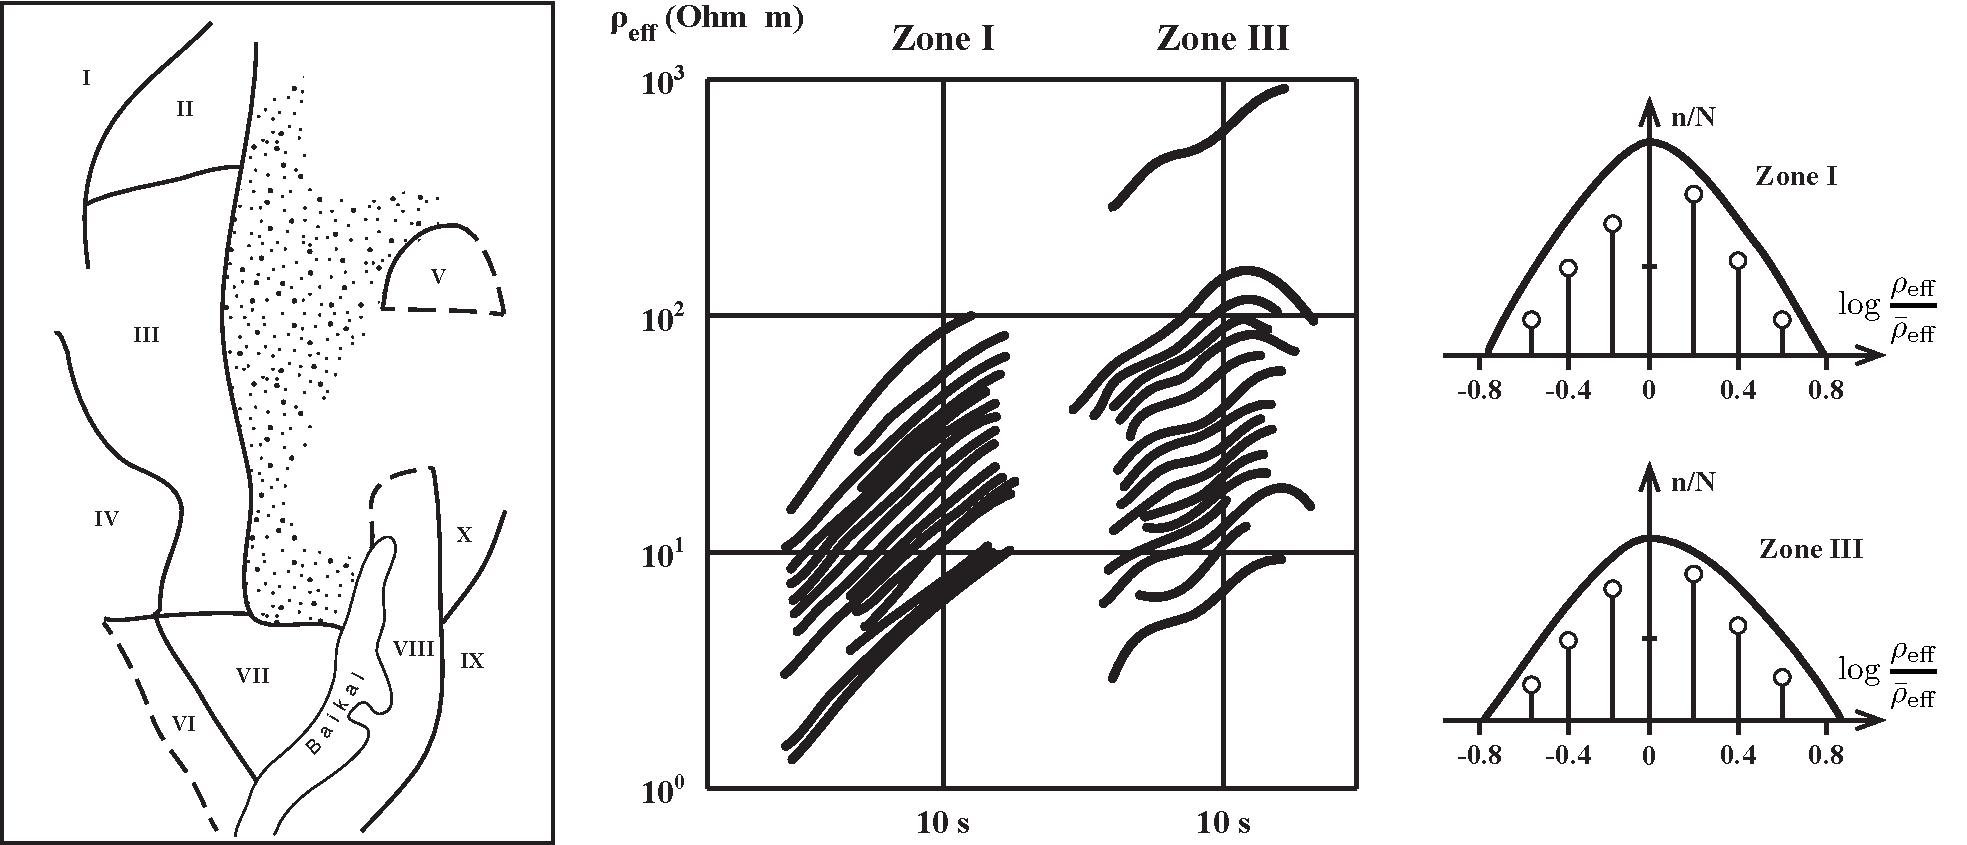
\includegraphics[width=5.5in]{\figdir/berdichevsky_result.pdf}
	\caption[Summary of \citet{berdichevsky1980a}]{(left) Map of Baikal region divided into regions (denoted by numbers), where each has the same conformal effective resistivity curves. (middle) The effective resistivity curves and (right) the distribution of the coefficient $K^i$  from data within Zone I and III \citep[after][]{berdichevsky1980a}.}
	\label{fig:berdichevsky_result}
\end{figure}
	

	
%% ==== ==== ==== ==== Distortion
% !TEX root = ../../phdthesis_tawatr.tex 

%% ==== ==== ==== ==== 
\section[Galvanic distortion]{Galvanic distortion}\label{sect:galvanic_distortion}

%	\begin{itemize}
%		\item \red{Introductory p.}
%		\item
		 Galvanic distorion is the alteration of electric field due to near-surface small-scale heterogeneity.  
%		\item
		 In theory, the distortion of the MT data may be both galvanic and inductive, but we can choose a proper period range so that only the galvanic distortion is considered \citep{groom1992a, utada2000a}.
%		\item
		 In contrast to marine cases, most of on-land MT observations suffer from galvanic distortion. 
%		\item
		 This section provides the physical principle of galvanic distortion, its mathematical formulation, and the galvanic distortion model or parameterization used in this work.
%	\end{itemize}
	
\begin{figure}[!h]
	\centering
	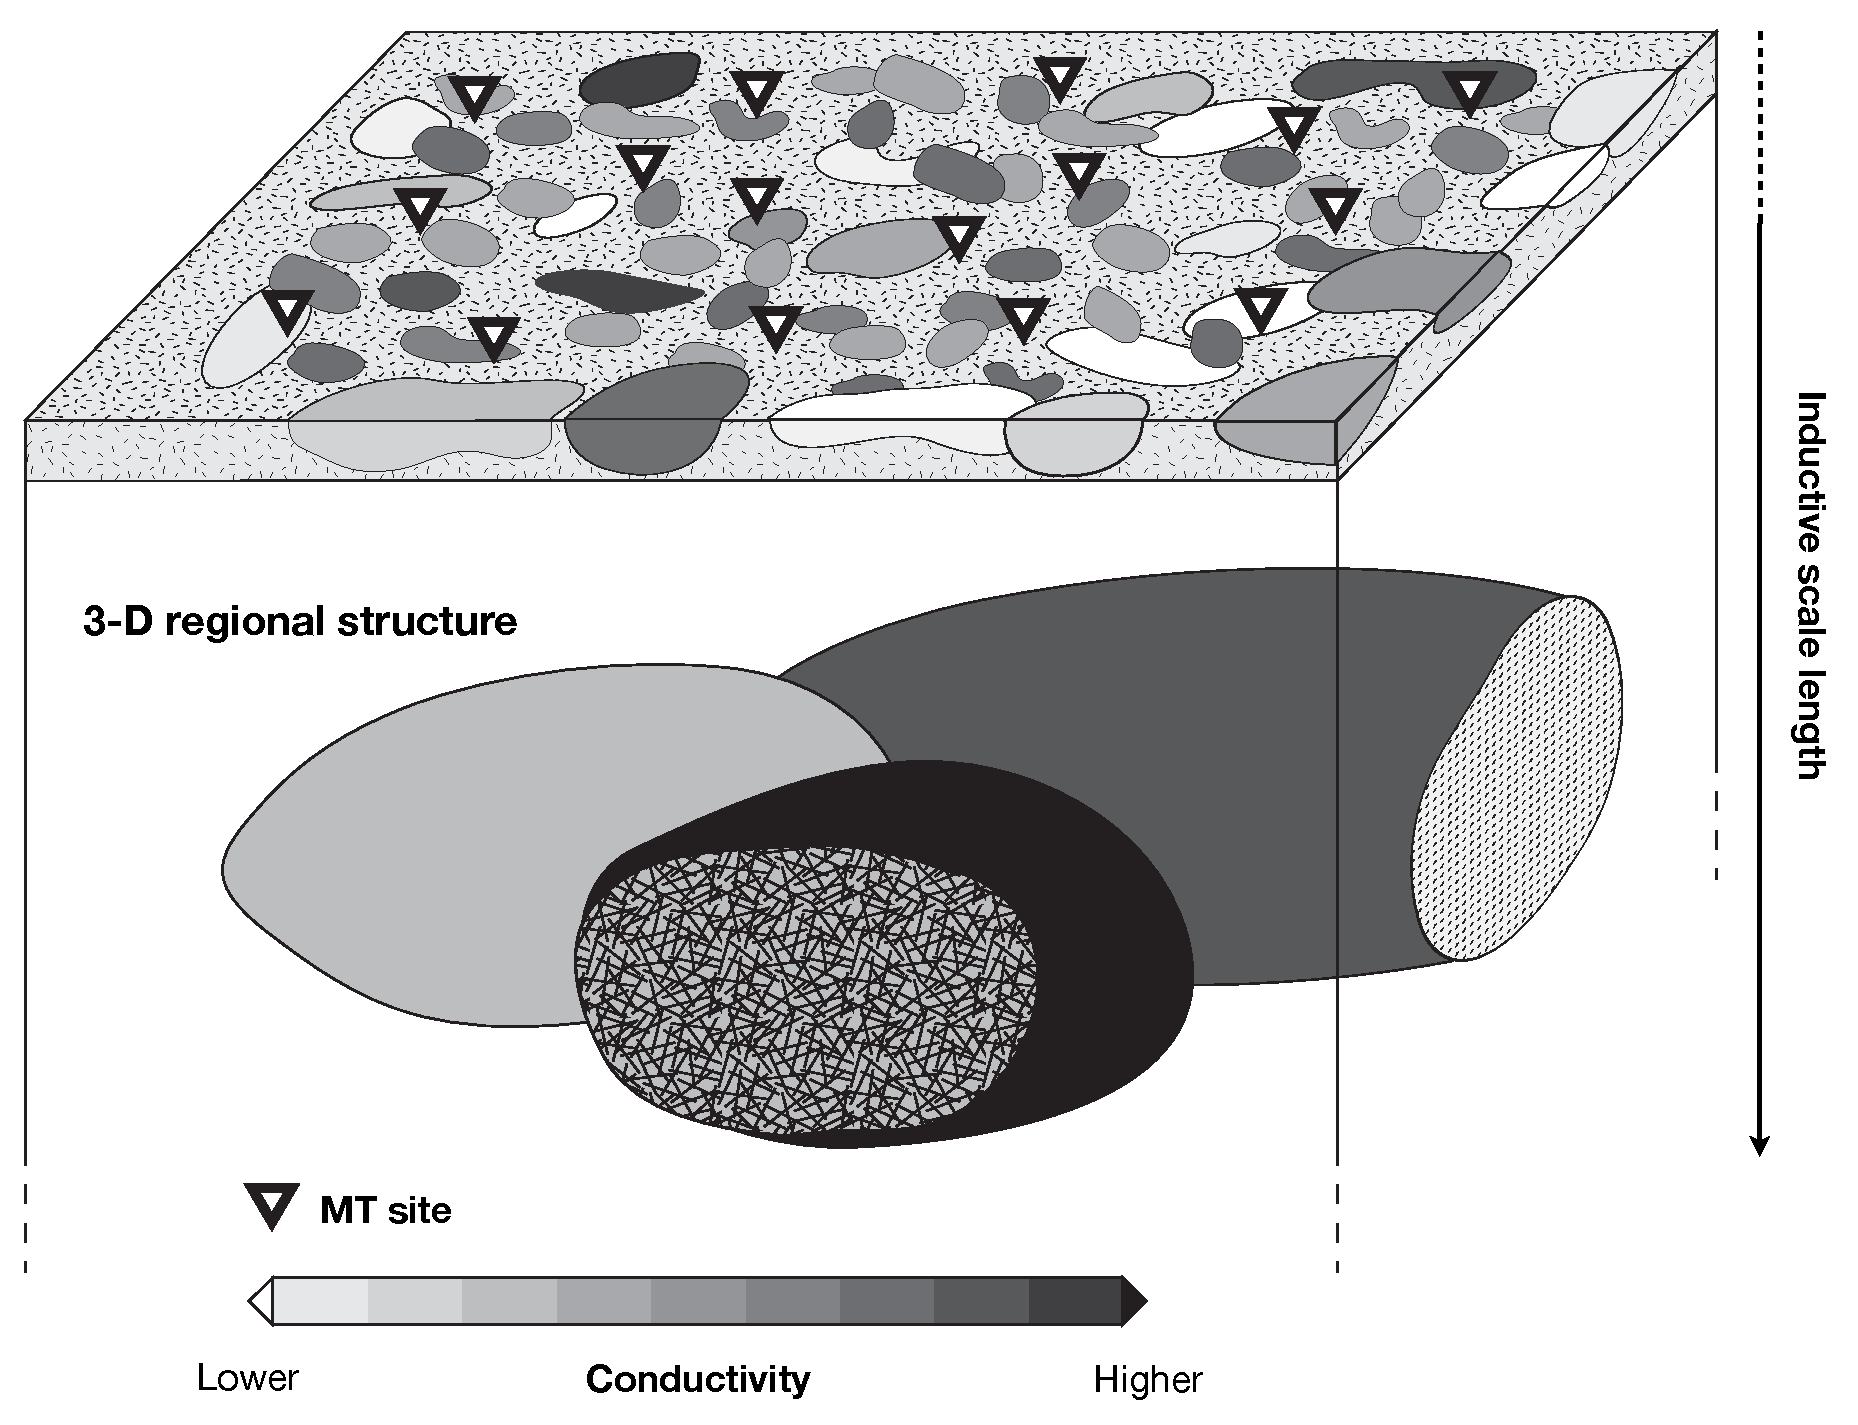
\includegraphics[width=5in]{\figdir/galvanicdistortion_model.pdf}
	\caption[A model of galvanic distortion in this study]{A model of galvanic distortion in this study. The model consists of 3D regional scale structure, which is of interest, and small-scale heterogeneities confined in the near-surface layer, which is shallower and thinner than the inductive scale length of interest \citep[after][]{utada2000a, rung-arunwan2016a}.}
	\label{fig:galvanic_distortion_model}
\end{figure}

%% ==== ==== ==== ==== 
\subsection{Galvanic distortion principle}
		% Theory of galvanic distortion
%	\begin{itemize}
%		\item 
		Following the formulation presented in \citet{groom1992a}; \citet{chave1994a} and \citet{utada2000a},
		this section provides the galvanic distortion principle based on electromagnetic scattering theory, which will leads to the mathematical representation of galvanic distortion.
		
%		\item 
		According to \citet{hohmann1975a}, the electric field observed at an arbitrary position $\rbf$, both internal and external to the scatterer, from a 3D heterogeneous medium can be expressed as
			\begin{equation} \label{eq:efield_int}
				\begin{split}
					\Ebf\fxr & = \Ebf_\Regional\fxr - i\omega\mu_0\sum_j\int_{V_j}  \,g(\rbf,\rbf')\,\delta\sigma_j(\rbf')\, \Ebf(\rbf') \, \dwrt V' \\
					& \quad + \nabla\, \frac{1}{\sigma_0}\, \div{\sum_j \int_{V_j} \,g(\rbf,\rbf')\,\delta\sigma_j(\rbf')\, \Ebf(\rbf') \, \dwrt V' },
				\end{split}
			\end{equation}
			where $V_j$ refers to each scattering body.
%			\red{
			Note that the quantities in Eq. \eqref{eq:efield_int} except the conductivity $\sigma_0$ and $\delta\sigma_j$ and the magnetic permeability $\mu_0$ are frequency dependent, but they are implicitly written.
%			}
%			\blueb{I am not sure how put the frequency dependence of these quantities before the equation. Then I put it here.}
			The anomaly conductivity contrast $\delta \sigma_j(\rbf')$ is defined by
			\begin{equation} \delta \sigma_j(\rbf') = \sigma_j(\rbf') - \sigma_0(\rbf'), 
			\end{equation}
			where $\sigma_j$ is the scatterer conductivity and $\sigma_0$  is the background or regional conductivity structure.
			The analytical expression of the Green's function of the uniform Earth is given by
			\begin{equation}
				g(\rbf,\rbf') = \frac{\expe{i\gamma_0 |\rbf-\rbf'|}}{4\pi|\rbf-\rbf'|},
			\end{equation}
			where $\gamma_0=\sqrt{i\omega\mu_0\sigma_0}$. The inductive scale length, or the electromagnetic skin depth, of the uniform background is 
			\begin{equation}\label{eq:idl_background}
				\lambda_0 = \frac{1}{|\Re\,\gamma_0|}.
			\end{equation}
			From the expression of the electric field \eqref{eq:efield_int}, the first term $\Ebf_\Regional\fxr$ is the field from the background structure, and the second and third terms denote the inductive and galvanic field components from each heterogeneity, which depends on size, conductivity contrast and \emph{inverse} distance.			
			But only the inductive term contains the frequency dependent part, which vanishes at long periods. 
			
			The integral solution for the magnetic field could then be obtained by applying Faraday's law to Eq. \eqref{eq:efield_int};
			\begin{equation}\label{eq:bfield_int}
				\Bbf\fxr = \Bbf_\Regional\fxr + \mu_0 \curl \sum_j \int_{V_j} g(\rbf,\rbf')\,\delta\sigma_j(\rbf')\,\Ebf(\rbf')\, \dwrt V', 
			\end{equation}
			In contrast to the electric field, the magnetic field \eqref{eq:bfield_int} contains only the inductive term due to the heterogeneity. The galvanic component vanishes because of the vector calculus identity that the curl of gradient of any scalar function is the zero vector. Therefore, the galvanic effect comes from the electric field only.
			
			% Induction number
			The contribution from each scattering body or distorter could be determined by the induction number $M_j$, 
			\begin{equation}
				M_j = \frac{L_j}{\lambda_j}.
			\end{equation}
			which is the ratio of its horizontal dimension $L_j$ to its inductive scale length 
			\begin{equation}\label{eq:idl_anomaly}
				\lambda_j=1/|\Re\,\gamma_j|,
			\end{equation}
			where $\gamma_j=\sqrt{i\omega\mu_0\delta\sigma_j}$.
%
			The distorters are generally small in size and then have very small induction numbers.
				If these distorters are confined to the near-surface layer, shallower and thinner than the background inductive scale length (Figure \ref{fig:galvanic_distortion_model}), they produce the \emph{visible} galvanic effect. 
			
			% Spatial aliasing
			Ideally, if we  have an infinitely dense MT survey and infinite band of data, all features could be explained by observation \citep{utada2000a}.			
			However, MT data is spatially insufficient because an MT array consisting of a limited number of sites is generally designed at least to cover the target structure with the typical site spacing that is able to resolve the smallest-scale target of interest.
			Therefore, the typical site spacing may be larger than the size of the distorters.
			The galvanic distorters inevitably cause spatial aliasing in MT data, i.e., both interesting and irrelevant structures are included in the observation. Such an effect is called galvanic distortion. 
			As it is impossible to recover original spatial features by using aliased data, the galvanic distorters are regarded as \emph{unresolvable} structure \citep{booker2014a}. In order to obtain the reliable results, some treatments or augmented approaches to handle the galvanic distortion are essential.
		
%		\red{HU CORRECTION UP TO HERE}
				
		% Draw the conclusion how it becomes real operator
%	\begin{itemize}
%			\item 
			The electric field solution in Eq. \eqref{eq:efield_int} could be simplified as 
			\begin{equation}\label{eq:efield_model}
				\Ebf\fxr = \Ebf_\Regional\fxr + \mbf{e}_\text{I}\fxr + \mbf{e}_\text{G}\fxr,
			\end{equation}
			where $\mbf{e}_\text{I}\fxr$ and $\mbf{e}_\text{G}\fxr$ represent the inductive and galvanic contributions from the scatterer. In the galvanic limit, Eq. \eqref{eq:efield_model} becomes
			\begin{equation}\label{eq:efield_model_approx}
				\Ebf\fxr \approx  \Ebf_\Regional\fxr  + \mbf{e}_\text{G}\fxr
			\end{equation}
			When the size of each scatterer is sufficiently small, the background electric field can be regarded as uniform inside the scatterer. The horizontal vector of the galvanic field $\mbf{e}_{\text{G},\text{h}}\fxr$ can be related to the undistorted horizontal background electric field $\Ebf_\Regional^\text{h}\fxr$ as
			\begin{equation}
				\mbf{e}_{\text{G},\text{h}}\fxr=\alpha \Ebf_{\Regional,\text{h}}\fxr,
			\end{equation}
			where $\alpha$ is a rank-2 real-valued tensor \citep[see][]{chave1994a}.
			The observed \emph{distorted} electric field (Eq. \ref{eq:efield_model_approx}) then becomes
			\begin{equation}
				\Ebf_\text{h}\fxr =  (\Ibf  + \alpha) \Ebf_{\Regional,\text{h}}\fxr = \Cbf\,\Ebf_{\Regional,\text{h}}\fxr,
			\end{equation}
			where $\Cbf$ is called the distortion operator, which is rank-2 real-valued tensor.
						
%	\end{itemize}

			
%		\item 
		Within the scope of galvanic distortion, the distorted impedance tensor is expressed as the product between the distortion operator $\Cbf$ and the regional (undistorted) impedance tensor $\ZbfUndistorted$:
		\begin{equation}\label{eq:z_distorted}
		\begin{split}
			\ZbfDistorted & =\Cbf\ZbfUndistorted, \\
			\ZDistortedMatrix & = \CMatrix\ZMatrixUndistorted \\
				& = \begin{bmatrix} 
						\Cxx\ZxxR + \Cxy\ZyxR & \Cxx\ZxyR + \Cxy\ZyyR \\
						\Cyx\ZxxR + \Cyy\ZyxR & \Cyx\ZxyR + \Cyy\ZyyR
					\end{bmatrix}
		\end{split}
		\end{equation}
		where the distortion operator {\Cbf} is a $2\times2$ matrix, the elements {\Cxx\ \Cxy\ \Cyx\ \Cyy} are real-valued and frequency-independent scalars.


%% ==== Attempts to galvanic distortion	 		 
%\begin{itemize}
%	\item 
	Several attempts have been made to handle the galvanic distortion problem. Here we briefly summarize some of them. The nature of solving the problem of galvanic distortion is an underdetermined problem. Some constraints or assumptions are necessary.
	For example, the tensor decomposition methods \citep[e.g.,][]{groom1989a, chave1994a, smith1995a, mcneice2001a} is viable under the assumption of 2D regional structure.
	\citet{gomez-trevino2014a} proposed the solution with the aid of rotational invariants, but it is limited to 2D.
%	\item
	Ideally, \citet{utada2000a} introduced the constraints from Faraday's law, but it is impractical in reality.
%	\item 
%	\red{
	The phase tensor \citep{caldwell2004a} and the vertical magnetic transfer function galvanic distortion-free solution. However, because of their absence of magnitude, the inversion based on the phase tensor and the vertical magnetic transfer function strongly depends on the starting models \citep{siripunvaraporn2009a, patro2013a, tietze2015a}. 
%	}
	Also, the vertical magnetic transfer function or tipper is another galvanic distortion-free response.
	However, the tipper is only sensitive to the lateral contrast in conductivity. Therefore the model inverted from the tipper relies on an intial or \emph{a priori} model.
%	\item 
%	\red{
%	However, the phase tensor-based inversion would give \citep{tietze2015a}
%	Some people might apply the constraints to the known structures, e.g., ocean, to get more reliable results from the phase-tensor-based inversion. \redb{see Kanda paper}}
%	\redb{Check the paper of Uyeshima and Tietze}
%	\item 
	Simultaneous inversion of MT data and galvanic distortion \citep[e.g.,][]{sasaki2006a, jones2011a, avdeeva2015a} is also a forthcoming approach. However, its implementation is rather complicated and still it does not fully solve the problem.
%\end{itemize}

%% ==== ==== ==== ====
%\subsection
%		Thus the definition of regional scale is different with different frequency range.

%% ==== ==== ==== ====
	\subsection[Groom--Bailey's framework]{Distortion operator parameterization: Groom--Bailey's framework}
%	\begin{itemize}
%		\item
		 The distortion operator $\Cbf$ can be treated in numerous ways. In this work, we adopted the Groom--Baileys' model of galvanic distortion, which is regarded as one of the standard models of galvanic distortion 
\citep[e.g.,][]{ chave1994a, mcneice2001a, chave2012a}.
		Its principle is briefly described as follows.
%		\parencite[e.g.,][]{chave1994a}[ and see also][]{chave2012a}

%		\item
		 Any $2\times2$ real-valued matrices {\Mbf} could be represented by the linear combination of the modifined Pauli spin matrices \citep{spitz1985a},
		\begin{equation}
			\Mbf = \alpha_0\SigmaZero+\alpha_1\SigmaOne+\alpha_2\SigmaTwo + \alpha_3\SigmaThree,
		\end{equation}
		where the coefficients $\alpha_{i=0,...,3}$ are arbitrary constants. The modifined Pauli spin matrices are
		\begin{equation}
			\SigmaZero=\SigmaZeroMat, \quad
			\SigmaOne=\SigmaOneMat, \quad
			\SigmaTwo=\SigmaTwoMat, \quad
			\SigmaThree=\SigmaThreeMat,
		\end{equation}
		which are mutually orthonormal. Based on these basis matrices,
		\citet{groom1989a} proposed a \emph{physically-based} parameterization of the distortion operator \Cbf, which will be referred to as Groom--Bailey's distortion model:
		\begin{equation}\label{eq:c_gtsa}
			\Cbf = \gain\Tbf\Sbf\Abf.
		\end{equation}
		The positive scalar {\gain} is called the site gain.
		By analogy to deformation theory of materials (Figure \ref{fig:gtes_vector}), the matrices {\Tbf}, {\Sbf} and {\Abf} are, respectively, the twist, shear, and splitting (or anisotropy, but later will be referred to splitting only) operators, which are $2\times2$ real-valued matrices. 
		They are given by
		\begin{equation}\label{eq:TSA_def}
			\begin{split}
				\Tbf & = \NT(\SigmaZero+\twistp\SigmaTwo) = \NT\Tmatrix, \\
				\Sbf & = \NS(\SigmaZero+\shearp\SigmaOne) = \NS\Smatrix, \\
				\Abf & = \NA(\SigmaZero+\splittingp\SigmaThree)  = \NA\Amatrix, \\
			\end{split}
		\end{equation}
		where \twistp, {\shearp}, and {\splittingp} are twist, shear, and splitting parameters; {\NT}, {\NS}, and {\NA} are the normalizing coefficients defined from the Frobenius norm of each distortion operator \citep[also see][]{bibby2005a}:
		\begin{equation}
				\NT = \frac{1}{\sqrt{1+t^2}}, \quad
				\NS = \frac{1}{\sqrt{1+e^2}}\quad \text{ and } \quad
				\NA = \frac{1}{\sqrt{1+s^2}}. 
		\end{equation}
		These normalizing coefficients are introduced to ensure that the power of the distorted electric fields is conserved.  
		
%		\item 
		The twist and shear parameters, {\twistp} and {\shearp}, can be physically represented by the twist and shear angles:
		\begin{equation}
			\begin{split}
				\twistp & = \tan \twista \\
				\shearp & = \tan \sheara 
			\end{split}
		\end{equation}

%% ==== Figure distored electric field vectors
\begin{figure}[!h]
	\centering
	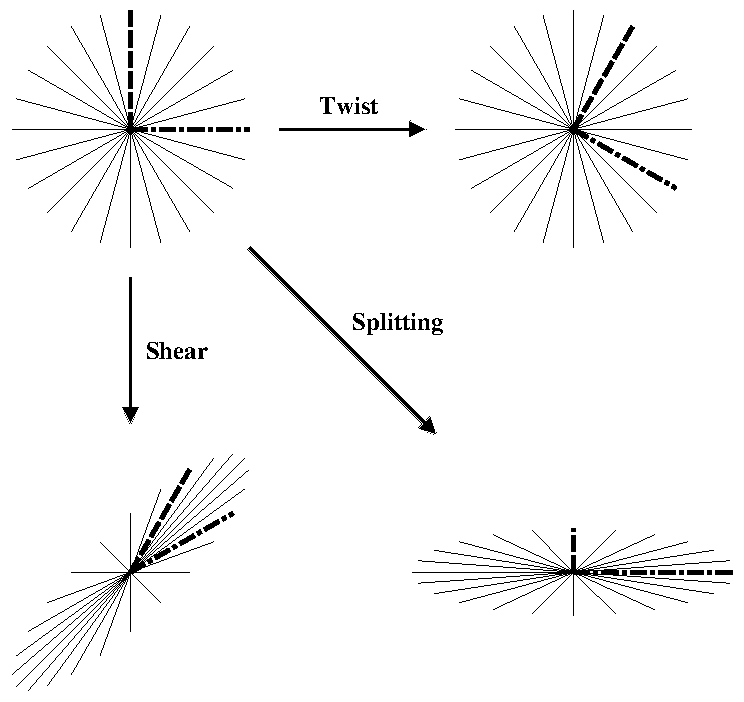
\includegraphics[width=4in]{\figdir/plot_uvec_crop.pdf}
	\caption[Effect of twist, shear and anisotropy operators on a family of unity vectors]{Effect of twist, shear and anisotropy operators on a family of unity vectors, where the twist shear and splitting parameters are $\tan 30^\circ$ \citep[after][]{groom1989a}.}
	\label{fig:gtes_vector}
	% Sketch to illustrate the effects of twist, shear and anisotropy. On the top is a group of unity vectors with 2 reference vectors in red and blue. On the bottom are the groups of vectors after application of (from left to right) twist (Eq. 2.114), shear (Eq. 2.113) and atnisotropy (Eq. 2.112). The black dashed lines indicate the original position and length of the two reference vectors (red and blue), which are now delocated and/or deformed. Redrawn from Groom (1988) and Groom and Bailey (1989).
\end{figure}
		
%		\item 
		By substituting the definitions of twist, shear, and splitting operators (Eq. \ref{eq:TSA_def}) into Eq. \eqref{eq:c_gtsa}, the explicit form of the distortion operator $\Cbf$ in terms of Groom--Bailey's distortion parameters is:		
		\begin{equation}\label{eq:c_gb}
			\Cbf = \CMatrix = \gain\NT\NS\NA\begin{bmatrix} (1+\splittingp)(1-\twistp\shearp) & (1-\splittingp)(\shearp-\twistp) \\
(1+\splittingp)(\shearp+\twistp) & (1-\splittingp)(1+\twistp\shearp) \end{bmatrix}.
		\end{equation}
		The distorted impedance could be calculated by substituting the distortion operator as expressed in Eq. \eqref{eq:c_gb} into Eq. \eqref{eq:z_distorted}.
%		\item 
		We can also write the the distortion operator $\Cbf$ as a linear combination of the modified Pauli spin matrices:
		\begin{equation}
			\Cbf = \cZero \SigmaZero + \cOne \SigmaOne + \cTwo\SigmaTwo + \cThree\SigmaThree,
		\end{equation}	
		where the coefficients $c_i$ are:
		\begin{equation}\label{eq:alphai_gb}
		\begin{split}
			\cZero & = \gain\, \NT\NS\NA\,(1-\shearp\splittingp\twistp), \\
			\cOne & = \gain\, \NT\NS\NA\,(\shearp+\splittingp\twistp), \\
			\cTwo & = \gain\, \NT\NS\NA\,(\shearp\splittingp+\twistp), \\
			\cThree & = \gain\, \NT\NS\NA\,(\splittingp-\shearp\twistp). \\
		\end{split}
	\end{equation}
%\gain\, \NT(\SigmaZero+\twistp\SigmaTwo) \, \NS(\SigmaZero+\shearp\SigmaOne) \, \NA(\SigmaZero+\splittingp\SigmaThree) \\
%			& =  \gain\, \NT\NS\NA\,( (1-\shearp\twistp\splittingp)\SigmaZero+(\shearp+\splittingp\twistp)\SigmaOne + (\twistp+\shearp\splittingp)\SigmaTwo + (\splittingp-\shearp\twistp)\SigmaThree) \\				

%		\item 
		It is also important to note that the distortion operators -- $\gain, \Tbf, \Abf$ and $\Sbf$ -- act differently on the impedance tensors (Figure \ref{fig:gtes_vector}). The site gain $\gain$ is a scalar. Hence the magnitude of the impedance tensor will be scaled up or down. The effect of site gain {\gain} is then called the \emph{static shift} -- frequency independent variation in the magnitude, or apparent resistivity, MT data. The twist, shear, and splitting operators, cause the geometrical change, changing the dimensionality of the impedance tensor, and the mixing among components of impedance tensor or called \emph{phase mixing}.
%		\textcolor{red}{[Citation for phase mixing]}. 
%	\end{itemize}



	

	


\clearpage

% !TEX root = ../../phdthesis_tawatr.tex 
\renewcommand{\thisdir}{_content/reg1d_method}
\renewcommand{\figdir}{\thisdir/_fig}
\chapter[Proposed Methods]{Estimating the regional mean conductivity profile} 
\label{chap:method}

In addition to the definition of the theoretical model of regional 1D conductivity profile (Eqs. \ref{eq:regional_mean_linear} and \ref{eq:regional_mean_log}), we describe the methods proposed in this thesis. First, we showed our finding that the ssq impedance is less sensitive to galvanic distortion when compared to the det impedance. Then, we reexamine the Berdichevsky average and redefine it with the ssq impedance. Lastly, we propose the galvanic distortion-related indicators -- the local and regional distortion indicators, and the apparent gains.

%\section{Theoretical model of the regional mean conductivity profile}
%\begin{itemize}
%	\item Present the definition of regional mean 1D.
%	\item \red{Do we need to recap it? I don't think so}
%\end{itemize}

\section[Distorted invariant impedances]{Effect of galvanic distortion on the rotational invariants: Algebraic derivation}\label{sect:distorted_invariants}
%\begin{itemize}
%	\item 
	In addition to the simple model of galvanic distortion over the det impedance by \citet{berdichevsky1980a}, \citet{gomez-trevino2013a} studied the effect of Groom--Bailey distortion parameters on the det and ssq impedances, but the study was limited to the 2D Earth.
%	\item 
	In this section, we provide the algebraic derivation of the distorted det and ssq impedances within the Groom--Bailey framework in the general case. 
	The expressions of the distorted det and ssq impedances in \citet{rung-arunwan2016a} are clarified and derived in terms of the matrix operation which is simple and intuitive.
%\end{itemize}

\subsection{Distorted det impedance}
%\begin{itemize}
%	\item
	 The determinant of the distorted impedance tensor is straightforward to derive by employing the multiplicative property of determinants. 
	First, we begin with the generalized form Eq. \eqref{eq:z_distorted}, 
		\begin{equation}\label{eq:detz_distorted_c}
			\begin{split}
				\det(\ZbfDistorted) & = \det(\Cbf\,\ZbfUndistorted) \\
								& = \det(\Cbf)\,\det(\ZbfUndistorted).
			\end{split}
		\end{equation}
%	\item 
	Applying the Groom--Bailey framework, Eq. \eqref{eq:detz_distorted_c} becomes
		\begin{equation}\label{eq:detz_distorted_gb}
			\begin{split}
				\det(\ZbfDistorted) & = \det(\gain\Tbf\Sbf\Abf)\det(\ZbfUndistorted) \\
				& = g^2 \det(\Tbf) \det(\Sbf) \det(\Abf) \det(\ZbfUndistorted) \\	
				& = g^2 \frac{1-e^2}{1+e^2} \frac{1-s^2}{1+s^2} \det(\ZbfUndistorted).
			\end{split}
		\end{equation}
%	\item 
	From Eq. \eqref{eq:zdet_def}, the distorted det impedances is then written as
	\begin{equation}\label{eq:zdet_distorted_gb}
		\ZdetDistorted = g\sqrt{\frac{1-e^2}{1+e^2} \frac{1-s^2}{1+s^2}}\,\ZdetUndistorted.
	\end{equation}
%	\item 
	Evidently, the distorted det impedance is biased downward by the splitting and shear parameters:
	\begin{equation}
		|\ZdetDistorted| = \gainp\,\sqrt{\frac{1-\shearp^2}{1+\shearp^2} \frac{1-\splittingp^2}{1+\splittingp^2}}\,|\ZdetUndistorted| \le \gainp\, |\ZdetUndistorted|
	\end{equation}
%	\item 
	Hence, using the det impedance may result in an underestimating the regional impedance by the shear and splitting effects.

	From Eqs. \eqref{eq:detz_distorted_c} and \eqref{eq:detz_distorted_gb}, the effect of galvanic distortion on the det impedance causes only the impedance scaling. 
	The expression in Eq. \eqref{eq:zdet_distorted_gb} also clarifies the coefficient $K_i$, which have no definition but the random quantity, in the galvanic distortion model of \citet{berdichevsky1980a} (Eq. \ref{eq:berdichevsky_galvanicdistortion_model}).
	
%	\item
	The virtue of using the det impedance is that its phase is distortion free, regardless of dimensionality of the earth. However, it may be problematic because the effect of site gain and splitting and shear parameters are indistinguishable. All of them can cause the shift in det apparent resistivity.
	
%	\item 
%\end{itemize}

%% ==== ==== Distorted ssq impedance
\subsection{Distorted ssq impedance}

	Owing to the Frobenius norm definition of the normalizing coefficients, $\NT\NS\NA$, and the Frobenius norm-like definition of ssq impedance, we are interested in examining the ssq impedance under galvanic distortion.
	As with the previous subsection, we begin deriving the distorted ssq in the generalized form of the distortion operator and then apply Groom--Bailey decomposition.
	The ssq of the distorted impedance tensor could be obtained by performing straightforward algebra, but here we chose to use the matrix operation.

	Starting from the product of the distorted impedance tensor,
	\begin{equation}\label{eq:z_distorted_prod}
		\begin{split}
			\transpose{{\ZbfDistorted}} \ZbfDistorted & = \transpose{\ZbfUndistorted}\transpose{\Cbf}\Cbf\ZbfUndistorted \\
			& = \transpose{\ZbfUndistorted}\transpose{(\cZero\SigmaZero+\cOne\SigmaOne + \cTwo\SigmaTwo + \cThree\SigmaThree)} (\cZero\SigmaZero+\cOne\SigmaOne + \cTwo\SigmaTwo + \cThree\SigmaThree)\ZbfUndistorted \\
			& =  \transpose{\ZbfUndistorted}\left[ \left(\cZero^2+\cOne^2+\cTwo^2+\cThree^2 \right)\SigmaZero + 2\left( \cZero\cThree + \cOne\cTwo \right) \SigmaThree + 2\left( \cZero\cOne - \cTwo\cThree \right)\SigmaOne \right] \ZbfUndistorted
		\end{split}
	\end{equation}
	Calculating trace of Eq. \eqref{eq:z_distorted_prod} to get the ssq of the distorted impedance tensor,
	\begin{equation}\label{eq:ssq_z_c}
		\begin{split}
		\ssq(\ZbfDistorted) & = \tracefunc{\transpose{\ZbfUndistorted}\transpose{\Cbf}\Cbf\ZbfUndistorted} \\
		& = \left(\cZero^2+\cOne^2+\cTwo^2+\cThree^2 \right) \tracefunc{\transpose{\ZbfUndistorted}\ZbfUndistorted} \\ 
		& \quad\quad + 2\left( \cZero\cThree + \cOne\cTwo \right) \tracefunc{\transpose{\ZbfUndistorted}\SigmaThree\ZbfUndistorted} \\
		& \quad\quad + 2\left( \cZero\cOne - \cTwo\cThree \right)\tracefunc{\transpose{\ZbfUndistorted}\SigmaOne\ZbfUndistorted} \\
		& = \left(\cZero^2+\cOne^2+\cTwo^2+\cThree^2 \right) \ssq(\ZbfUndistorted) \\
		& \quad\quad + 2\left( \cZero\cThree + \cOne\cTwo \right) ({\ZxxR}^2+{\ZxyR}^2-{\ZyxR}^2-{\ZyyR}^2) \\
		& \quad\quad + 2\left( \cZero\cOne - \cTwo\cThree \right) \, 2(\ZxxR\ZyxR+\ZxyR\ZyyR)		
		\end{split}
	\end{equation}
	Note that Eq. \eqref{eq:ssq_z_c} is free of $\SigmaTwo$, which defines the twist operator.
%
	Substituting the coefficients $c_i$ in Eq. \eqref{eq:alphai_gb} into Eq. \eqref{eq:ssq_z_c} and perfoming modest algebra, we obtain:
	\begin{equation}\label{eq:ssq_z_distorted_gtes}
		\begin{split}
		\ssq(\ZbfDistorted) & = g^2\NT^2\NS^2\NA^2\, (1+\twistp^2) (1+\shearp^2) (1+\splittingp^2)\, \left[\phantom{\frac{1}{2}} \right. \\
		& \quad\quad \left. \ssq(\ZbfUndistorted)+\frac{2\splittingp}{(1+\splittingp^2)}  ({\ZxxR}^2+{\ZxyR}^2-{\ZyxR}^2-{\ZyyR}^2) \right.\\
		& \quad\quad \left. + \frac{4\shearp\,(1-\splittingp^2)}{(1+\shearp^2)(1+\splittingp^2)} ({\ZxxR}{\ZyxR}+{\ZxyR}{\ZyyR}) \right] \\
		& = g^2\left[ \ssq(\ZbfUndistorted)+\frac{2\splittingp}{(1+\splittingp^2)} ({\ZxxR}^2+{\ZxyR}^2-{\ZyxR}^2-{\ZyyR}^2) \right. \\
		& \quad\quad \left. + \frac{4\shearp\,(1-\splittingp^2)}{(1+\shearp^2)(1+\splittingp^2)} ({\ZxxR}{\ZyxR}+{\ZxyR}{\ZyyR})  \right]
		\end{split}
	\end{equation}
The effect of the distortion parameters on the ssq impedance depends on the dimensionality of the structure. The splitting parameter will be effective if the Earth is not 1D (the 2nd and 3rd terms in Eq. \ref{eq:ssq_z_distorted_gtes}), while the shear parameter becomes effective when the Earth is 3D only (the 3rd term in Eq. \ref{eq:ssq_z_distorted_gtes}).
	%
	Note that \citet{gomez-trevino2013a} also obtained the expression similar to Eq. \eqref{eq:ssq_z_distorted_gtes}.
%	, in which their discussion were limited to the 2D regional structure only.
	
	As with the det impedance, the ssq impedance is the rotational invariant and hence independent of the twist parameter.
	Adopting Eq. \eqref{eq:zssq_def}, for simplicity we write the distorted ssq impedance:
	\begin{equation}\label{eq:zssq_distorted_gtes}
		\ZssqDistorted = \gain \ZssqDistortedExGain,
	\end{equation}
	where
	\begin{equation}\label{eq:zssq_distorted_gtes_exgain}
	\begin{split}
		\ZssqDistortedExGain & = \frac{1}{\sqrt{2}}\left[ \ssq(\ZbfUndistorted)+\frac{2\splittingp}{(1+\splittingp^2)} ({\ZxxR}^2+{\ZxyR}^2-{\ZyxR}^2-{\ZyyR}^2) \right. \\
		& \quad\quad \left. + \frac{4\shearp\,(1-\splittingp^2)}{(1+\shearp^2)(1+\splittingp^2)} (\ZxxR\ZyxR+\ZxyR\ZyyR)  \right]^\frac{1}{2}
	\end{split}
	\end{equation}

%	\begin{itemize}
%		\item
\begin{comment}
		 The contribution from the MT impedance components in the 2nd and 3rd terms is generally weak, unless the very strong inductive effect, e.g., coastal effect, is recognized or the data is heavily distorted. Consequently, we may assume
	\begin{equation}
		\ZssqDistortedExGain \approx \ZssqUndistorted
	\end{equation}
%		\item 
		The virtue of the ssq impedance appears when the Earth is 1D, where the impedance tensor is anti-symmetric (Eq. \ref{eq:z_cond_1d}). 
		The 2nd and 3rd terms in Eq. \eqref{eq:zssq_distorted_gtes_exgain} then vanish, and the distorted ssq impedance becomes
		\begin{equation}
			\ZssqDistorted = \gain \ZssqUndistorted.
		\end{equation}
		The observed ssq impedance is only affected by the site gain.
		In general, the ssq impedance is less biased by the distortion parameters, which is in contrast to the det impedance that is always biased downward by the shear and splitting parameters. 
		According to these findings, we derive two implications -- estimating the regional 1D impedance and the galvanic distortion-related indicators -- from the det and ssq impedances. 

\end{comment}

%		The benefit of using the ssq impedance in redefining the Berdichevsky average will be demonstrated in the next section.
%	\end{itemize}
	
%	Writing $\Cbf=\gain\Tbf\Sbf\Abf$ as a linear combination of the modified Pauli spin matrices,
%		\begin{equation}
%			\begin{split}
%				\Cbf & = g\Tbf\Sbf\Abf \\
%					& = g\, \NT(\SigmaZero + \twistp\SigmaTwo)
%			\end{split}
%		\end{equation}

%% ==== 
\section{Redefining the Berdichevsky average}\label{sect:berdichevsky_redefined}
%\begin{itemize}
%	\item 
	Although using the ssq impedance may reduce the bias due to the splitting and shear parameters, the site gain $\gain$ remains the problem. 
	In this section, we will show that the average approach is one strategy to relieve the problem of site gain.
	Also, to show the difference between using the average det impedance and the average ssq impedance, we reexamine the Berdichevsky average within the Groom--Bailey framework, and redefine the Berdichevsky average with the ssq impedance.	

%	\item
	Given that $N$ MT observations were made, we rewrite the Berdichevsky average (Eq. \ref{eq:berdichevsky_avg_def}) as the geometric average of impedances, 
		\begin{equation}\label{eq:zdet_mean}
				\ZdetDistortedMean\fxomega = \left[ \prod\limits_{i=1}^{N}\, \ZdetDistorted\fxriomega\,\right ]^\frac{1}{N},
		\end{equation}
		where $\rbf_i$ denotes the position vector of the $i$th observation. 
	Substituting the distorted det impedance Eq. \eqref{eq:zdet_distorted_gb} into Eq. \eqref{eq:zdet_mean},
	\begin{equation}
		\ZdetDistortedMean\fxomega = \left[ \prod\limits_{i=1}^{N}\, \gainpi\,\sqrt{\frac{1-\shearpi^2}{1+\shearpi^2} \frac{1-\splittingpi^2}{1+\splittingpi^2}}\, \ZdetUndistorted\fxriomega\right ]^\frac{1}{N},
	\end{equation}
	where $\gainpi$, $\shearpi$ and $\splittingpi$ are the site gain, shear and splitting parameters at the $i$th station.
	On the basis of the central limit theorem and assuming that the site gain is log-normally distributed \citep{berdichevsky1980a}, the arithmetic average of site gains from a number of observations in a logarithmic scale is approximately zero \citep[see also][]{degroot-hedlin1991a, ogawa1996a}. In other words, the geometric average of site gains becomes unity:
	\begin{equation}
		 \prod\limits_{i=1}^{N}\, g_i  \rightarrow 1.
	\end{equation}
	Approximately, the average det impedance then becomes
	\begin{equation} \label{eq:zdet_mean_apprx}
	\begin{split}
		\ZdetDistortedMean\fxomega & \approx \left[ \prod\limits_{i=1}^{N}\, \sqrt{\frac{1-\shearpi^2}{1+\shearpi^2} \frac{1-\splittingpi^2}{1+\splittingpi^2}}\, \ZdetUndistorted\fxriomega\right ]^\frac{1}{N} \\
		& \approx \left[ \prod\limits_{i=1}^{N}\, \sqrt{\frac{1-\shearpi^2}{1+\shearpi^2} \frac{1-\splittingpi^2}{1+\splittingpi^2}} \right]^\frac{1}{N} \ZdetUndistortedMean\fxomega,
	\end{split}
	\end{equation}
	where the average regional det impedance 
	\begin{equation}
		\ZdetUndistortedMean\fxomega = \left[ \prod\limits_{i=1}^{N}  \ZdetUndistorted\fxriomega \right]^\frac{1}{N}.
	\end{equation}
	Averaging the impedance and applying the central limit theorem would help relieve the problem of site gain.
	However, the remaining coefficient of splitting and shear parameters, which is always less than unity, will underestimate the regional det impedance in terms of apparent resistivity. 
	In other words, the Berdichevsky average may lead to an overestimated model of the regional mean 1D conductivity profile. 
	%
	However, \citet{baba2010a} successfully applied the Berdichevsky average to marine MT data after showing that the galvanic distortion is negligible.
%	\item One benefit from averaging the impedance is that the problem of site gain is relieved.
%	\item This statistical characteristic of Berdichevsky average urged us to seek for another candidate that can reliably estimate the regional impedance.
%	\item As seen in Section \ref{sect:XXX}, the ssq impedance is less biased by galvanic distortion.
	
%	\item
	 Next, we redefine the Berdichevsky average with the ssq impedance. As the ssq impedance is less sensitive to the distortion parameters, the average ssq impedance is expected to yield the reliable estimate of the regional mean 1D conductivity profile. Writing the average ssq impedance as 
	\begin{equation}\label{eq:zssq_mean}
				\ZssqDistortedMean\fxomega = \left[ \prod\limits_{i=1}^{N}\, \ZssqDistorted\fxriomega\,\right ]^\frac{1}{N}.
	\end{equation}
	and substituting the distorted ssq impedance (Eq. \ref{eq:zssq_distorted_gtes}) into Eq. \eqref{eq:zssq_mean} gives 
	\begin{equation}\label{eq:zssq_mean_sub}
		\ZssqDistortedMean\fxomega = \left[ \prod\limits_{i=1}^{N}\, \gainpi\, \ZssqDistortedExGain\fxriomega\right ]^\frac{1}{N}.
	\end{equation}
%\end{itemize}

As with Eq. \eqref{eq:zdet_mean_apprx}, the central limit theorem is applied in averging site gain. 
If we average the impedance from a large number of observations covering an sufficiently large area, we may assume the effect of the 2nd and 3rd terms in Eq. \eqref{eq:zssq_distorted_gtes_exgain} becomes negligible. The average ssq impedance (Eq. \ref{eq:zssq_mean_sub}) becomes
\begin{equation}\label{eq:zssq_mean_apprx}
		\ZssqDistortedMean\fxomega \approx \ZssqUndistortedMean\fxomega,
\end{equation}
	where the average regional ssq impedance 
	\begin{equation}
		\ZssqUndistortedMean\fxomega = \left[ \prod\limits_{i=1}^{N}  \ZssqUndistorted\fxriomega \right]^\frac{1}{N}.
	\end{equation}
	Therefore, the average ssq impedance would give the good estimate of the regional mean 1D conductivity profile.

%In 1D situation, 
%\begin{equation}
%	\Zssq = \Zdet = \ZOneD,
%\end{equation}
%where $\ZOneD$ is the regional 1D impedance.



\section{Indicating the galvanic distortion}\label{sect:indicators}

In addition to estimating the regional mean conductvity profile, the combination of the det and ssq impedances would help determine the existence and strength of galvanic distortion contained in an MT dataset. 

\subsection{Local and regional distortion indicators}
Employing the fact that the effect of galvanic distortion on the det and ssq impedances are different, 
the local distortion indicator is defined as the squared ratio of the det impedance to the ssq impedance
\begin{equation}\label{eq:gamma_local_def}
	\gammai\fxomega = \frac{\ZssqDistorted\fxriomega^2}{\ZdetDistorted\fxriomega^2}.
\end{equation}
Applying the expressions for $\ZssqDistorted$ and $\ZdetDistorted$ in Eqs. \eqref{eq:zdet_distorted_gb} and \eqref{eq:zssq_distorted_gtes}, we obtain 
\begin{equation}
 	\gammai\fxomega = \frac{\gainpi^2\, \ZssqDistortedExGain\fxriomega^2}{\displaystyle \gainpi^2\,  \frac{1-\shearpi^2}{1+\shearpi^2} \frac{1-\splittingpi^2}{1+\splittingpi^2}\, \ZdetUndistorted\fxriomega^2}. 
\end{equation}
The presence of galvanic distortion can be examined by the consistency between the vertical magnetic transfer function and the lateral gradients of MT impedance \citep{utada2000a, rung-arunwan2016a}. The importance of the local distortion indicator exists in the separation of the site gain.
%As defined in this way, the local distortion indicator is intrinsically independent of site gain. 

In general cases, we may approximate the local distortion indicator as:
\begin{equation}\label{eq:gamma_approx}
	\gammai\fxomega \approx \frac{1+\shearpi^2}{1-\shearpi^2} \frac{1+\splittingpi^2}{1-\splittingpi^2}\, \frac{\ZssqUndistorted\fxriomega^2}{\ZdetUndistorted\fxriomega^2} \approx \frac{1+\shearpi^2}{1-\shearpi^2} \frac{1+\splittingpi^2}{1-\splittingpi^2}.
\end{equation}
The local distortion indicator is expressed as the product of the coefficient of distortion parameters and the difference between the ssq and det impedances.
The former is real-valued and frequency independent, and larger than unity if the data is distorted, while the latter is generally complex-valued and frequency-dependent. The difference between the det and ssq impedances is generally small; consequently, it may be ignored.
In an 1D situation, the local distortion indicator becomes
\begin{equation}\label{eq:gamma_1d_analytic}
	\gammai = \frac{1+\shearpi^2}{1-\shearpi^2} \frac{1+\splittingpi^2}{1-\splittingpi^2}.
\end{equation}
This ratio is the real-valued number indicating the strength of shear and splitting parameters. The stronger the galvanic distortion, the greater the local distortion indicator.
But if there is no distortion, the local distortion indicator becomes unity in the 1D situation.

In general, if the local distortion indicator was found to be real-valued and weakly frequency independent, the 1D regional structure may be assumed. The magnitude of the local distortion indicator denotes the strength of galvanic distortion posed in the data. 
%
If the local distortion indicator is varied (frequency dependent) about some constant magnitude, the distorted 3D data is suggested. 

%% ==== Mean local distortion indicator
	Further, we also define the mean local distortion indicator $\gammaimean$ by averaging the local distortion indicator over the given period range so as to relieve the frequency dependent part, which is mainly due to the underlying structure. 
%
Given that at the $i$th stations the number of periods is $M$, the mean local distortion indicator is given by averaging the real part of the local distortion indicator:
\begin{equation}\label{eq:gamma_local_mean_def}
	\gammaimean = \left[\prod\limits_{j=1}^{M} \Re\,\gammai(\omega_j) \right]^\frac{1}{M}.
\end{equation}
%
Only the real part is used in order to conform with the assumption that the galvanic distortion operator is real. 
This single-valued parameter is able to represent the galvanic distortion strength at an MT station and also ease analysing data from a number of MT stations. 

%% ==== ==== ==== ==== Regional distortion indicator
In addition to the local distortion indicator (Eq. \ref{eq:gamma_local_def}), we can determine how strongly the dataset is distorted using the regional distortion indicator, which is defined as the geometric mean of the local distortion indicators:
\begin{equation}\label{eq:gamma_regional_def}
	\gammaR\fxomega = \left[ \prod\limits_{i=1}^N \gammai\fxomega \right]^\frac{1}{N}  
\end{equation}
Substituting the approximation in Eq. \eqref{eq:zdet_mean_apprx} into Eq. \eqref{eq:zssq_mean_apprx}, we get 
\begin{equation}
\begin{split}
	\gammaR\fxomega & \approx \left[ \prod\limits_{i=1}^N \frac{1+\shearpi^2}{1-\shearpi^2} \frac{1+\splittingpi^2}{1-\splittingpi^2}\,  \right]^\frac{1}{N}  \frac{\ZssqUndistortedMean\fxriomega^2}{\ZdetUndistortedMean\fxriomega^2} \\
	& \approx \left[ \prod\limits_{i=1}^N \frac{1+\shearpi^2}{1-\shearpi^2} \frac{1+\splittingpi^2}{1-\splittingpi^2} \right]^\frac{1}{N}.
\end{split}
\end{equation}

%% ==== Paragraph about the regional distortion indicators
%\redb{Regional distortion indicator}

%\begin{itemize}
%	\item 
	By averaging the local distortion indicators, the contribution of the difference between the ssq and det impedances is diminished.
%	\item 
	The regional distortion indicator is expected to be real and frequency independent, and its magnitude represents the effect of the shear and splitting parameters on average. 
	As with the local distortion indicator, the larger the magnitude of the regional distortion indicator, the stronger the galvanic distortion.
%	\item 
	In some areas, if the near-surface layer is highly heterogenous, strong galvanic distortion is expected and the regional distortion indicator would help quantify its strength.
	If the MT dataset is strongly distorted, the proper treatment or removal of galvanic distortion may be necessary.
%\end{itemize}



\subsection{Apparent gains}
In addition to determining the strength of the shear and splitting parameters, the apparent gain was introduced to determine the magnitude of site gain, which generally claimed to be undeterminable without other independent information \citep{groom1993a, bibby2005a}.  
%
Here we show that estimating the site gain is plausible from a set of MT data.

%The static shift removal based on other data
%\citep[e.g.,][]{jones1988a, sternberg1988a}

As the averaging approach and assuming the central limit theorem relieves the problem of site gain, the apparent gains could be defined from the ratio of individual invariant impedance to the average impedance.
As two rotational invariants are of interest, we then examine two apparent gains, 
the apparent det and ssq gains: 
\begin{equation}\label{eq:gdet_def}
	\gdeti\fxomega = \frac{\ZdetDistorted\fxriomega}{\ZdetDistortedMean\fxomega}
\end{equation}
and
\begin{equation}\label{eq:gssq_def}
	\gssqi\fxomega = \frac{\ZssqDistorted\fxriomega}{\ZssqDistortedMean\fxomega}.
\end{equation}

%% ==== 1-D and general
In the 1D Earth, we will have
\begin{equation}
	\gdeti = \gainpi \sqrt{\frac{1-\shearpi^2}{1+\shearpi^2}\frac{1-\splittingpi^2}{1+\splittingpi^2}} \bigg/ \left[ \prod\limits_{i=1}^{N}\, \sqrt{\frac{1-\shearpi^2}{1+\shearpi^2} \frac{1-\splittingpi^2}{1+\splittingpi^2}} \right]^\frac{1}{N} 
\end{equation}
and
\begin{equation}
	\gssqi = \gainpi 
\end{equation}
If the apparent det and ssq gains are real and almost frequency independent, we may assume the earth is likely 1D. The magnitude of the apparent ssq gain would give a good estimate of the actual site gain.

In general, the apparent det gain is obtained by substituting the expressions for $\ZdetDistorted$ and $\ZdetDistortedMean$  (Eqs. \ref{eq:zdet_distorted_gb} and \ref{eq:zdet_mean_apprx}) into Eq. \eqref{eq:gdet_def}:
\begin{equation}
\begin{split}
	\gdeti\fxomega 
	& \approx \gainpi \sqrt{\frac{1-\shearpi^2}{1+\shearpi^2}\frac{1-\splittingpi^2}{1+\splittingpi^2}}\,  \ZdetUndistorted \fxriomega \bigg/ \left[ \prod\limits_{i=1}^{N}\, \sqrt{\frac{1-\shearpi^2}{1+\shearpi^2} \frac{1-\splittingpi^2}{1+\splittingpi^2}} \right]^\frac{1}{N}\, \ZdetUndistortedMean\fxomega\\
	 & \approx \gainpi \sqrt{\frac{1-\shearpi^2}{1+\shearpi^2}\frac{1-\splittingpi^2}{1+\splittingpi^2}} \bigg/ \left[ \prod\limits_{i=1}^{N}\, \sqrt{\frac{1-\shearpi^2}{1+\shearpi^2} \frac{1-\splittingpi^2}{1+\splittingpi^2}} \right]^\frac{1}{N}.
\end{split}
\end{equation}
The apparent ssq gain is obtained by substituting the expressions for $\ZssqDistorted$ and $\ZssqDistortedMean$  (Eqs. \ref{eq:zssq_distorted_gtes} and \ref{eq:zssq_mean_apprx}) into Eq. \eqref{eq:gssq_def}:
\begin{equation}
\begin{split}
	\gssqi\fxomega & \approx \gainpi \ZssqDistortedExGain\fxriomega \bigg/  \ZssqUndistortedMean\fxomega \\
		& \approx \gainpi \\
\end{split}
\end{equation}
%\redb{check the approximation again!}

Whether the Earth is 1D or not, the shear and splitting parameters systematically affect the apparent det gain. If the distortion at the individual station is stronger than the average, the apparent det gain will underestimate the actual site gain. 
%
Therefore the apparent det gain is either an overestimate or an underestimate.


To estimate the site gain for each station, we propose to calculate the mean apparent det and ssq gains $\gdetimean$ and $\gssqimean$ by averaging the real part of the apparent gains over the period range of interest.
Given that at each stations the number of periods is $M$, the mean apparent gains are:
\begin{equation}\label{eq:gdet_mean_def}
	\gdetimean = \left[\prod\limits_{j=1}^{M} \Re\,\gdeti(\omega_j) \right]^\frac{1}{M}
\end{equation}
and
\begin{equation}\label{eq:gssq_mean_def}
	\gssqimean = \left[\prod\limits_{j=1}^{M} \Re\,\gssqi(\omega_j) \right]^\frac{1}{M}
\end{equation}
%The aim of averaging the apparent gains is to flatten out frequency dependent part due to the 3D effect contained in the data.
Averaging would help flatten the frequency dependent features due to the underlying heterogeneity.
The mean apparent ssq gain are expected to be a good estimate of the site gain.




\clearpage
% !TEX root = ../../phdthesis_tawatr.tex 
\newcommand{\gtes}{(\gainp,\twistp,\shearp,\splittingp)}
\renewcommand{\thisdir}{_content/reg1d_synthetic_1d}
\renewcommand{\figdir}{\thisdir/_fig}
\chapter[Synthetic Experiments and Discussion]{Synthetic experiments and Discussion}
\label{chap:synthetic}

In this chapter, we test the proposed methods (as described in Chapter \ref{chap:method}) using the average ssq impedance to estimate the regional mean 1D conductivity profile and deriving galvanic distortion-related indicators through synthetic examples. 
%
Synthetic 1D and 3D models are used, and the galvanic distortion was simulated with the random distortion parameters -- $\gainp, \twistp, \shearp$ and $\splittingp$. 
%
As we introduce the theoretical model of regional mean 1D conductivity profile (Eqs. \ref{eq:regional_mean_linear} and \ref{eq:regional_mean_log}), we examined if it is consistent with the model of regional mean 1D conductivity profile estimated from the average ssq impedance. 

\section[1D examples]{Estimating a model of regional mean 1D profile: 1D example}\label{sect:example_1d}

%\begin{itemize}
%	\item 
	In this work, the synthetic layered-Earth model (Figure \ref{fig:lyrearth_model}) was made based on \citet{jones1999a}, which has the main feature of resistive upper crust (3.5--14.8 km depth) and conductive lower crust (14.8--33.3 km depth). This feature is commonly found in the continental crust \citep{jones1999a}.
%	\item 
	The corresponding MT response was calculated in the period range of (Figure \ref{fig:lyrearth_resp}) using the analytic solution \citep{constable1987a}.
%	\item 
	The heterogeneity embedded in the lower crust layer is detectable in this period range, while any structures confined in the near-surface layer -- a few kilometers or less, which is shallower and thinner than the inductive scale length of interest -- are considered to be the galvanic distorters.
%\end{itemize}

%% ==== Figure: The layer earth model
	\begin{figure}[t]
		\centering
		\subfigure[]{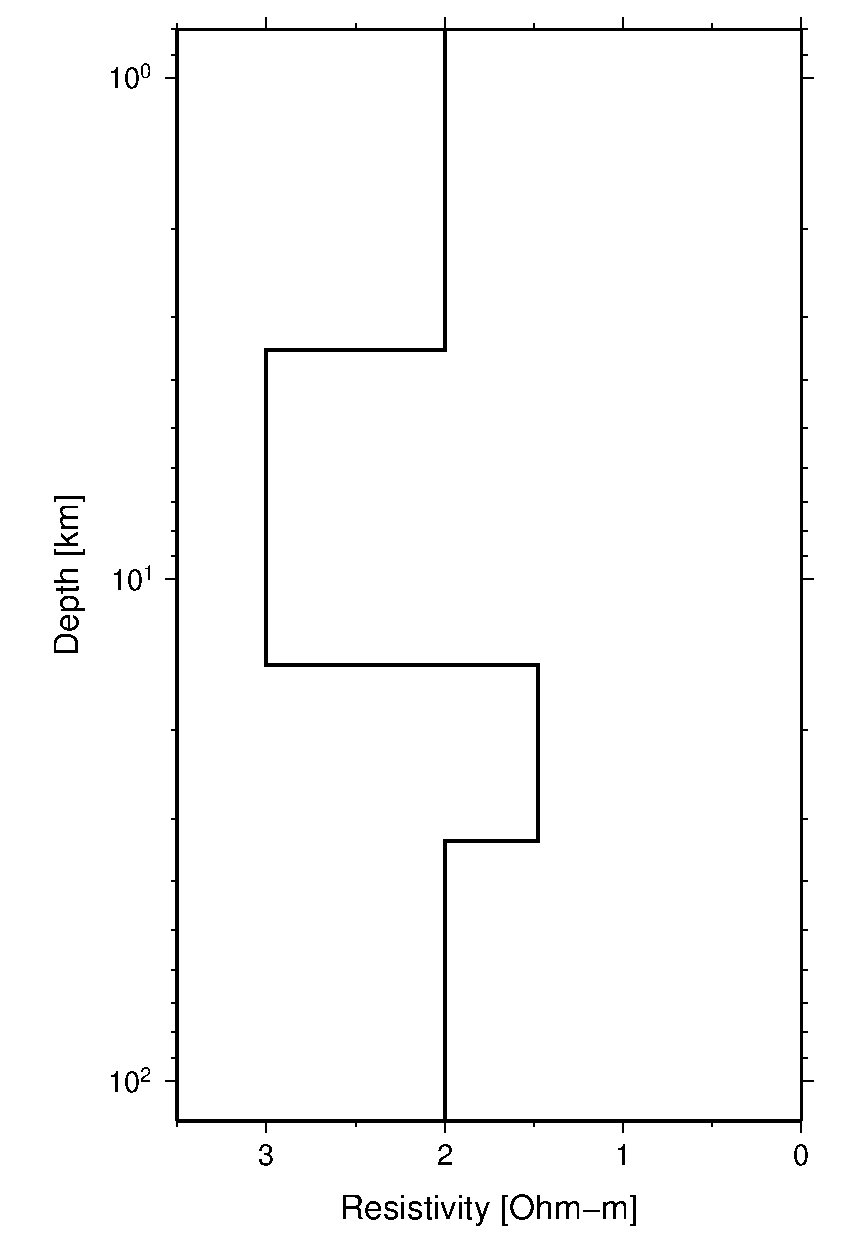
\includegraphics[scale=\plotinvmodelscale]{\figdir/model_lyr11a_cropped.pdf}
		\label{fig:lyrearth_model}
		}
		\subfigure[]{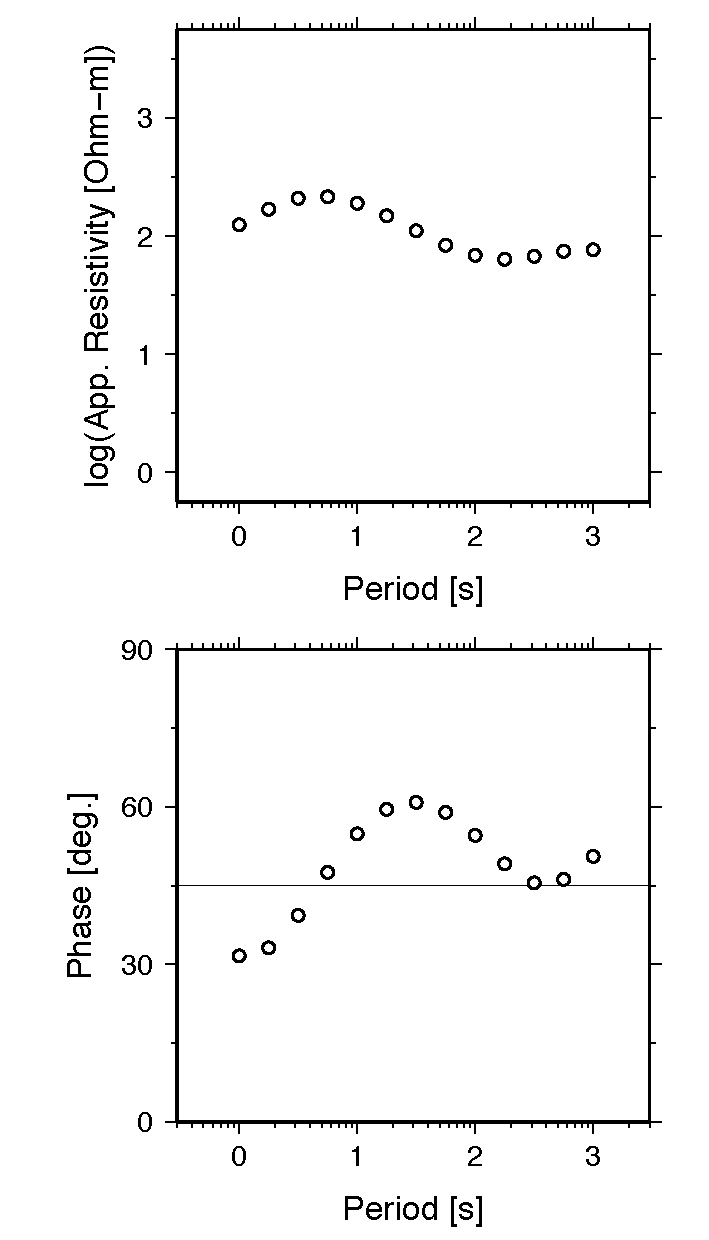
\includegraphics[scale=\plotmtrespscale]{\figdir/mesh-m01a-lyr11a_mt_arsphs_inv.pdf}
		\label{fig:lyrearth_resp}
		}
		\caption[Layered-earth model used in this study and corresponding response]{\subref{fig:lyrearth_model} Layered-Earth model used in this work. \subref{fig:lyrearth_resp} Corresponding MT response (apparent resistivity and phase).}\label{fig:lyrearth_resp}
	\end{figure}

%\begin{itemize}
%	\item 
	As described earlier, the near-surface distorters cause spatial aliasing in the data.
%	\item 
	The distortion parameters in the Groom--Bailey framework -- site gain $\gainp$, twist $\twistp$, shear $\shearp$ and splitting $\splittingp$ parameters -- can reasonably be assumed to be random \citep[e.g.,][]{avdeeva2015a}. 
%	\item 
	Given that the MT array consists of 25 MT stations in our synthetic tests, 25 sets of real-valued parameters $\gtes$ are generated from the normal distribution.
	Also, to quantify the galvanic distortion strength, the standard deviation (SD) used in the normal distribution ranges from 0.1--0.5 (Figure \ref{fig:dparam}). Note that when the SD was greater than 0.3, the randomly generated numbers were less likely to comply with the theoretical normal distribution, and more like the uniform distribution.
	We further assume that each set of distortion parameters has the mean of zero and is within $(-1,+1)$. Note that the random site gain was made in an logarithmic scale.
	Eventually, we have five MT datasets, 25 stations each, distorted with different galvanic distortion strength. The distorted impedances are calculated using Eq. \eqref{eq:z_distorted} by applying these random parameters to the 1D impedance (as shown in Figure \ref{fig:lyrearth_resp}).
%\end{itemize}

%%% ==== Figure: Distortion parameter plot and its distribution
	\begin{figure}[t]	
		\centering
		\subfigure[]{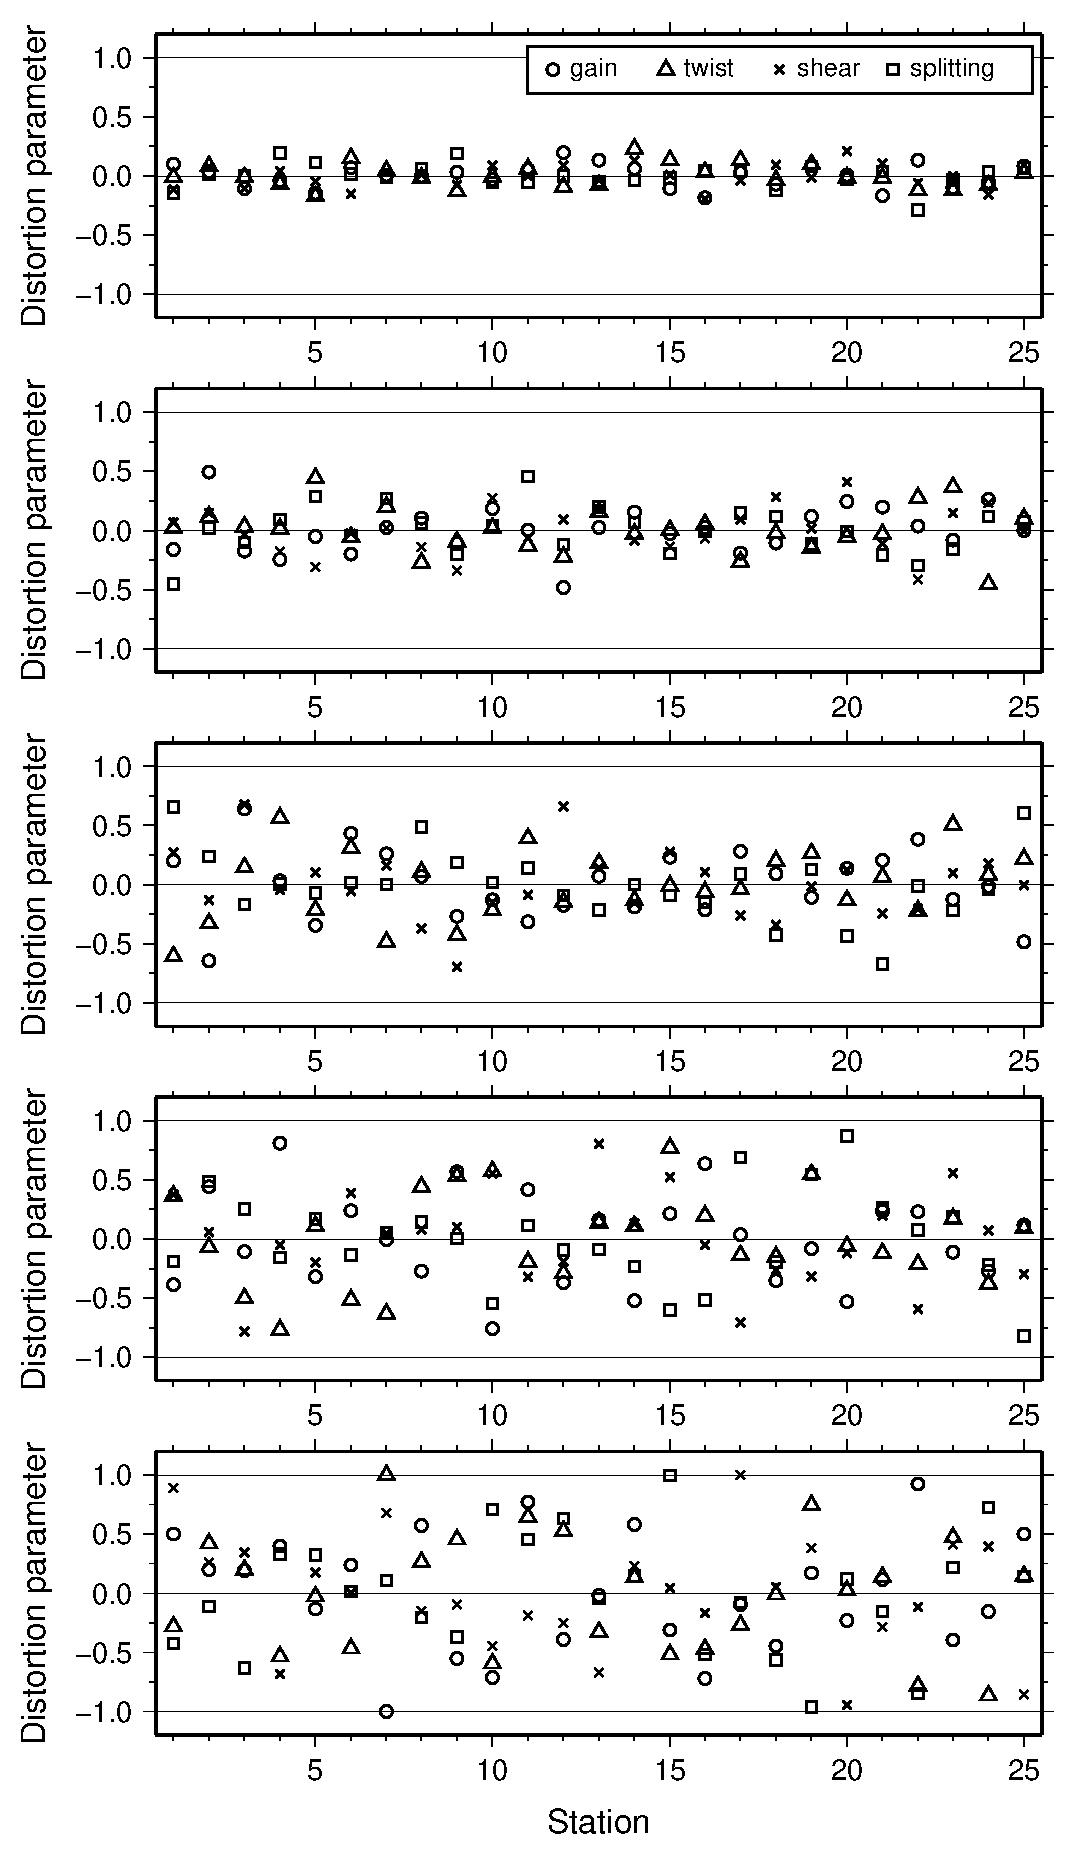
\includegraphics[scale=0.3]{\figdir/gtes.pdf}
		\label{fig:dparam_value}
		}
		\subfigure[]{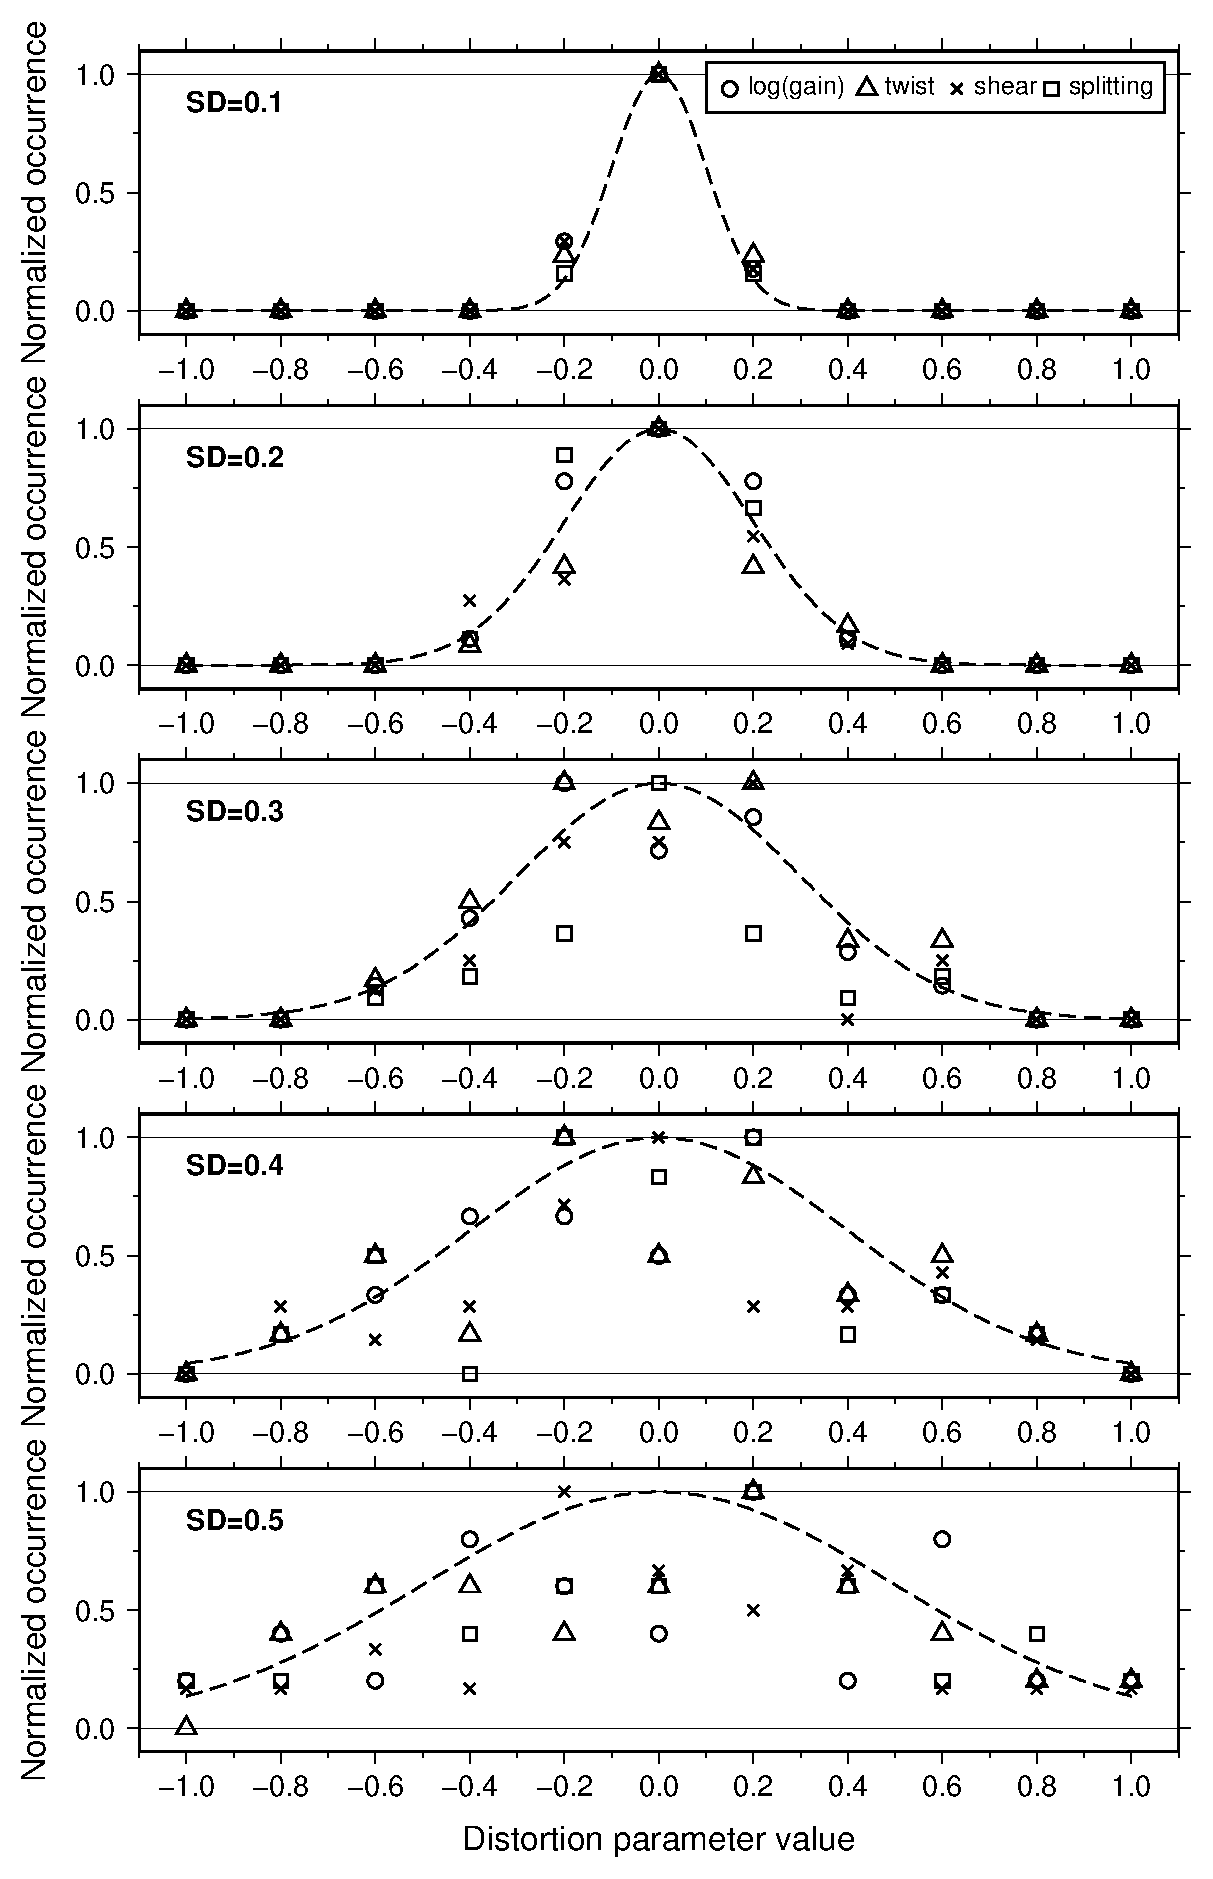
\includegraphics[scale=0.3]{\figdir/gtes_hist2.pdf}
		\label{fig:dparam_hist}
		}
		\caption[Distortion parameters and their distribution]{\subref{fig:dparam_value} Random distortion parameter values generated from the normal distribution with different SDs. \subref{fig:dparam_hist} Distribution of the distortion parameters. The normalized occurrence is the number of occurrences divided by the maximum number of occurrences at a single parameter value. Each distribution is compared with the probability density function of the theoretical normal distribution for the given SD (dashed lines).}
		\label{fig:dparam}
	\end{figure}
	
%% ==== Results: Individual
% \red{-- Individual --}
 
%\begin{itemize}
%	\item 
	In the 1D Earth, the galvanic distortion causes no phase mixing, but only a static shift in magnitude of the MT components (Figure \ref{fig:resp1d_example_distorted_zij}), whereas the galvanic distortion, as proven, only causes the static shift in the rotationally invariant impedances (Figure \ref{fig:resp1d_example_distorted_zinv}). The MT data in this example is distorted with $\gtes$ of $(1.20,0.11,-0.37,0.49)$.
%	\red{Note that the $xx$ phase  }
%	\item 
%	The example of data in Figure \ref{fig:resp1d_example_distorted} distorted with $\gtes=(1.20,0.11,-0.37,0.49)$ . 
	In this example, the synthetic site gain $\gainp$ is greater than unity. Therefore the ssq impedance is shifed upward. As described in Section \ref{sect:distorted_invariants}, the site gain provides the same effect on the det and ssq impedances. Hence the det impedance is also supposed to be shifted upward, but here it is biased downward due to the shear and splitting parameters so that its magnitude is less than the undistorted impedance. 
%	\item 


	
		
%% ====	
	As the distortion parameters are randomly generated, the rotational invariant impedances are irregularly shifted (Figure \ref{fig:resp1d_individual_all_distorted_sd3a}), which resembles the results in \citet{berdichevsky1980a} (Figure \ref{fig:berdichevsky_result}). 
%	\item 
	The shift in the ssq impedance is solely due to the site gain, but the shift in the det impedance also includes the shear and splitting parameters. 
	As mentioned, this behaviour could be problematic because the effect of the shear and splitting parameters and the site gain is indistinguishable, if the det impedance is chosen.
%\end{itemize}



%% ==== Results: Average
% \red{-- Average --}
 
%\begin{itemize}
%	\item
	To examine the effect of galvanic distortion strength on the regional mean impedance, the average det and ssq impedances for each distorted dataset (Figure \ref{fig:resp1d_avg_distorted}) were calculated using Eqs. \eqref{eq:zdet_mean} and \eqref{eq:zssq_mean}, respectively. Here, the error bar is the standard deviation of the data and therefore represents the level of dispersion of the sounding curves. The large error bars correspond to strong galvanic distortion strengths. For example, the dataset distorted with an SD of 0.5 has the largest error bar. 
%	\item 
	At the same strength of galvanic distortion, the average det impedances appear to be more dispersed than the average ssq impedances, because the shear and splitting parameters also affect the det impedance. 
%	\item 
	From the results, the average det impedance is biased downward by the galvanic distortion, although its effect is not noticeable when the SD of the distortion parameters is less than 0.2.
	On the contrary, the average ssq impedances remain the same at all galvanic distortion strengths.
	This is consistent with the theoretical derivation that the average ssq impedance would give the unbiased approximation of the model of the regional mean 1D conductivity profile \citep{rung-arunwan2016a}.
%\end{itemize}

%%% ==== Figure: Distored 1D response example
	\begin{figure}[t]
		\centering
		\subfigure[]{
		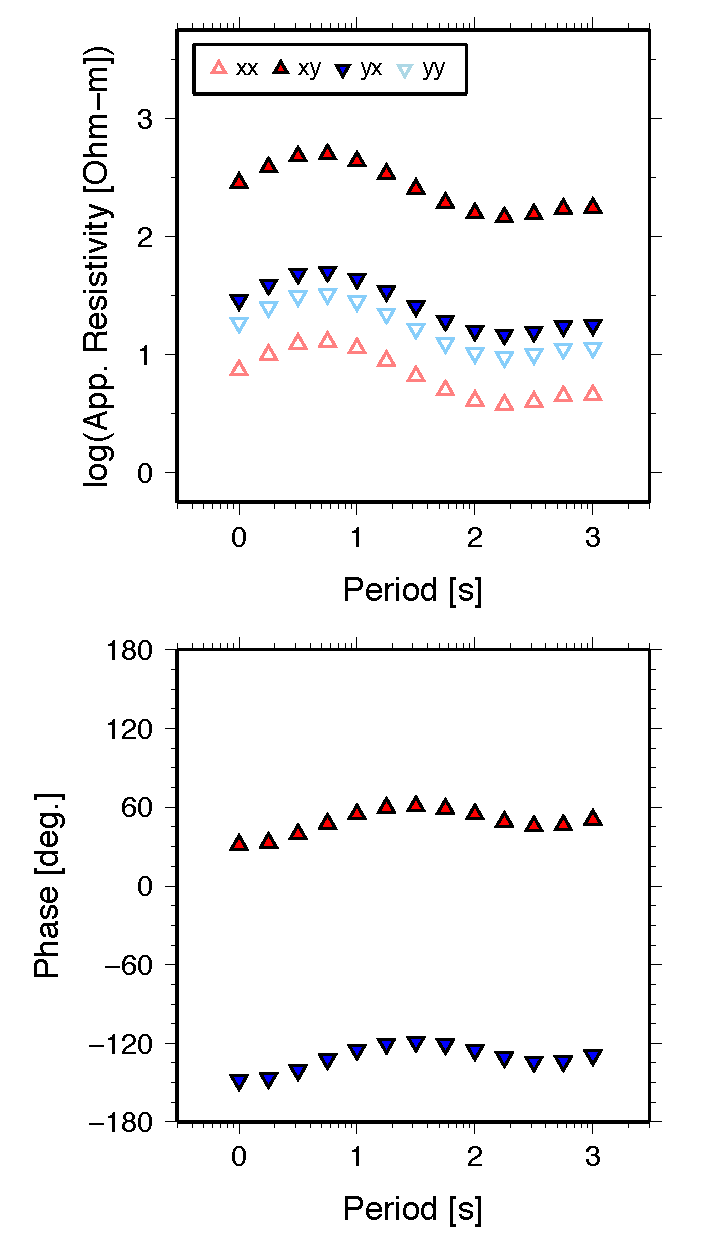
\includegraphics[scale=\plotmtrespscale]{\figdir/lyr11a_syn0203_mt_arsphs.pdf}
		\label{fig:resp1d_example_distorted_zij}
		}
		\subfigure[]{
		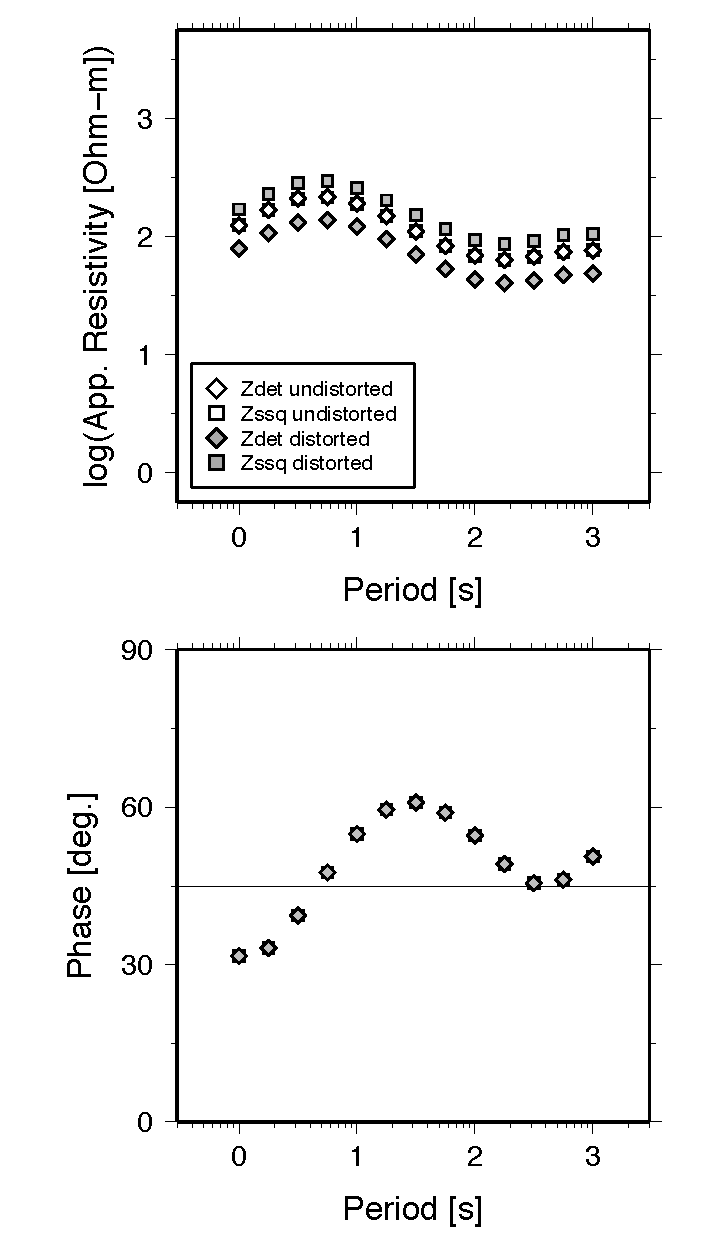
\includegraphics[scale=\plotmtrespscale]{\figdir/lyr11a_syn0203_zinv.pdf}
		\label{fig:resp1d_example_distorted_zinv}
		}
	\caption[Example of distorted 1D MT data and corresponding invariant impedances]{(a) Components of the 1D MT impedance distorted with $(g, t, e, s) = (1.20, 0.11, -0.37, 0.49)$. (b) Corresponding det (diamonds) and ssq (squares) impedances.}
	\label{fig:resp1d_example_distorted}
	\end{figure}
	
%% ==== Figure: Distored 1D response individual all sd3a
\begin{figure}[t]
	\centering
	\subfigure[]{
		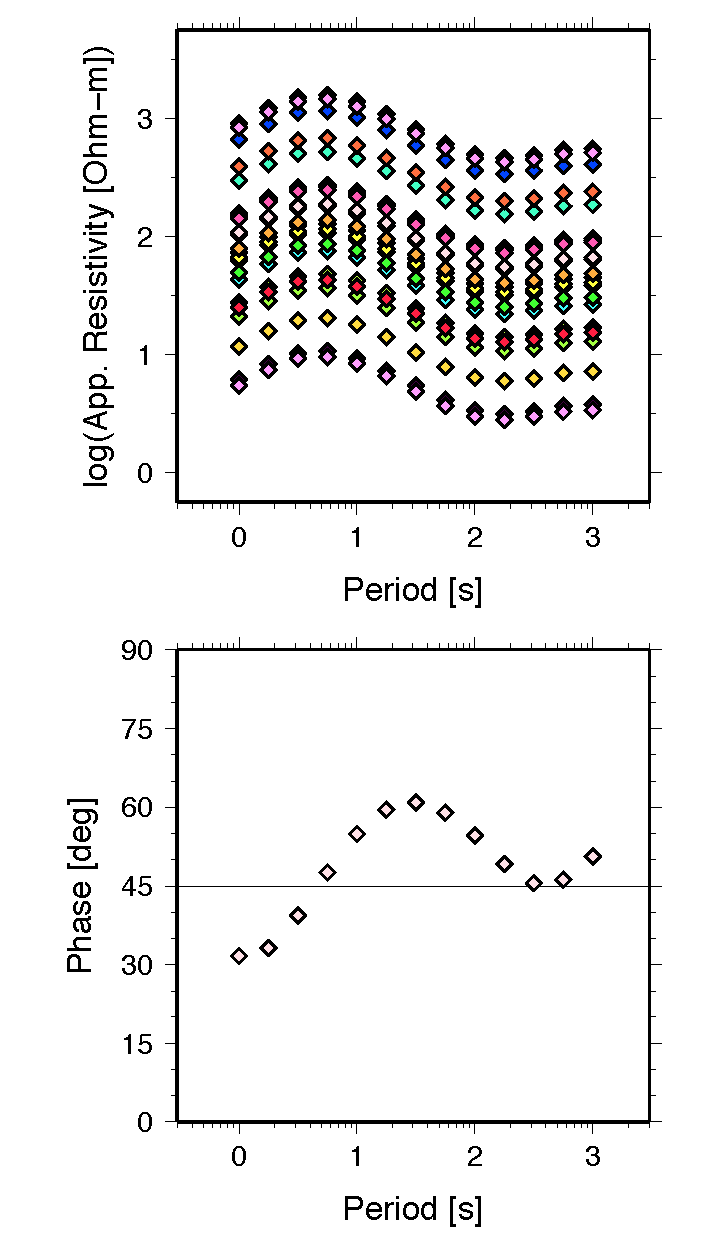
\includegraphics[scale=\plotmtrespscale]{\figdir/lyr11a_n25_d13a_distorted-sd3a-gtes_zinv_det_arsphs.pdf}
		\label{fig:resp1d_individual_all_distorted_sd3a_det}
	}
	\subfigure[]{
		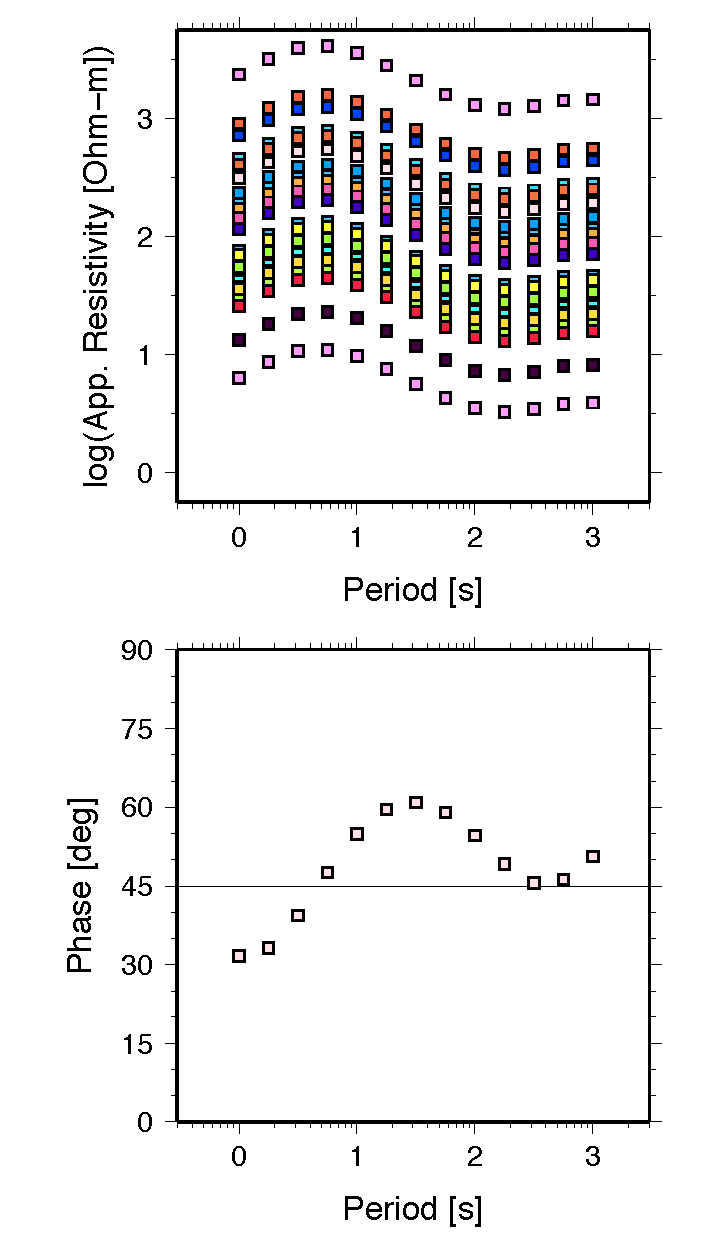
\includegraphics[scale=\plotmtrespscale]{\figdir/lyr11a_n25_d13a_distorted-sd3a-gtes_zinv_ssq_arsphs.pdf}
		\label{fig:resp1d_individual_all_distorted_sd3a_ssq}
	}
	\caption[Example of distorted det and ssq impedances from distorted 1D MT dataset]{Distorted (a) det and (b) ssq impedances from the 1D example, where a set of distortion parameters with an SD of 0.3 was applied. Each station is represented by a different symbol color.}
	\label{fig:resp1d_individual_all_distorted_sd3a}
\end{figure}
%% ==== Figure: Distored 1D response individual average
\begin{figure}[t]
	\centering
	\subfigure[]{
		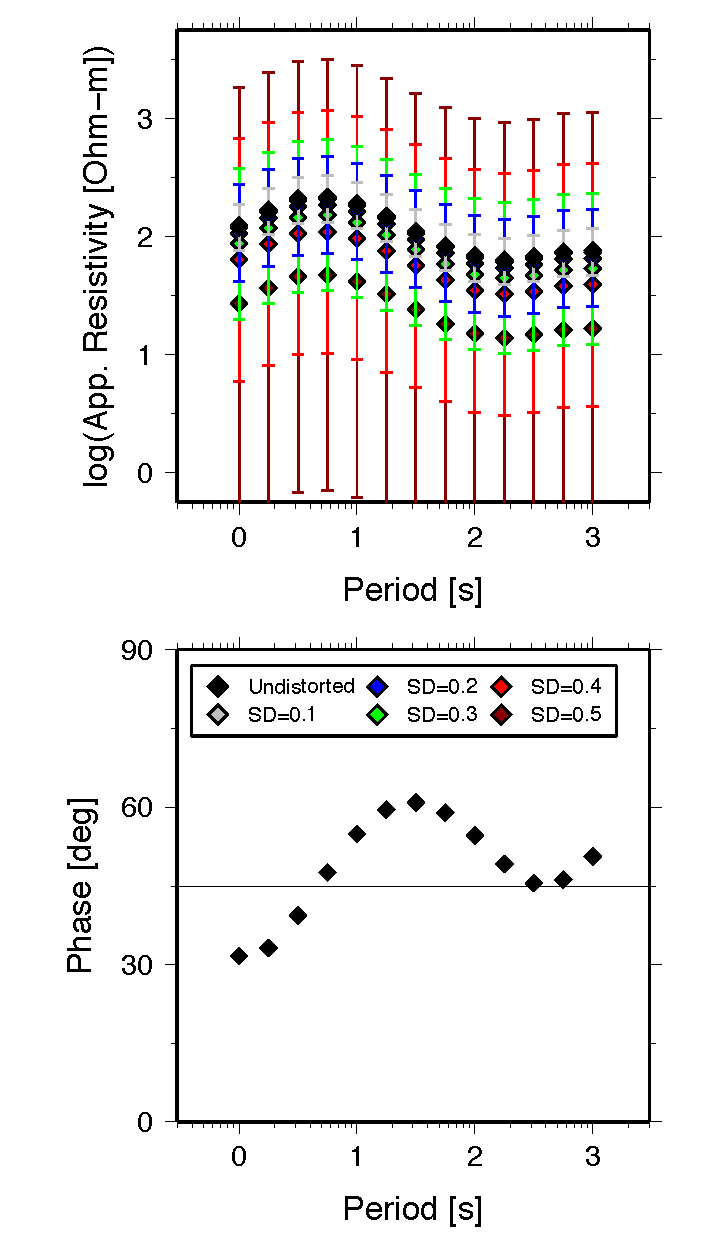
\includegraphics[scale=\plotmtrespscale]{\figdir/lyr11a_d13a_distorted-sdxa_mt_det.pdf}
		\label{fig:resp1d_avg_distorted_det}
	}
	%
	\subfigure[]{
		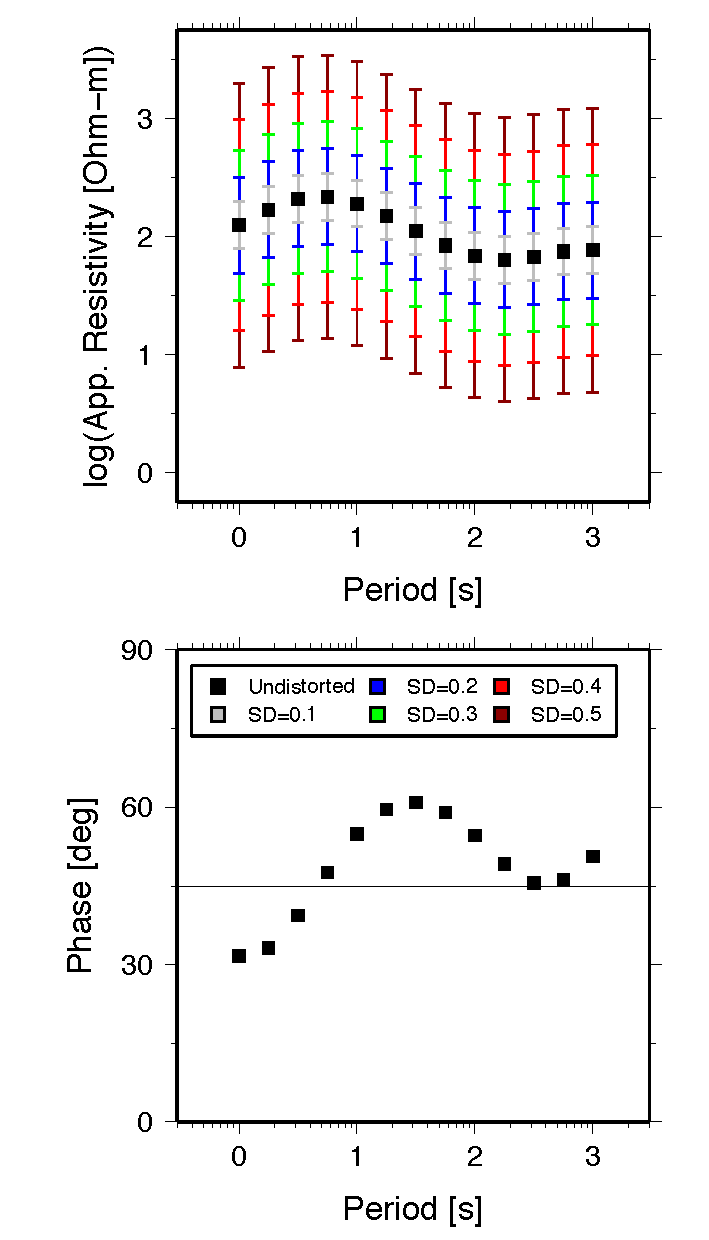
\includegraphics[scale=\plotmtrespscale]{\figdir/lyr11a_d13a_distorted-sdxa_mt_ssq.pdf}
		\label{fig:resp1d_avg_distorted_ssq}
	}
	\caption[Average det and ssq impedances from 1D MT datasets distorted with different galvanic distortion strengths]{Average (a) det and (b) ssq impedances from the 1D datasets distorted with different galvanic distortion strengths.}
	\label{fig:resp1d_avg_distorted}
\end{figure}

%% ==== Results Inverted model
% \red{-- Inverted models --}
 
% \begin{itemize}
%	\item 
	In this work, the Occam 1D inversion \citep{constable1987a} is used to yield the 1D models, in which the second derivative of the conductivity with respect to the depth is penalized. 
	The errors of the apparent resistivity and phase applied in the inversion were fixed at 2.3\% and 0.66$^\circ$, respectively. All inverted models shown in this work fit the data within a root mean square (RMS) error of unity.
%	\item 
	The inverted models from the average det impedances will be less resistive or more conductive than the true structure, particularly when the galvanic distortion is strong.
	On the other hand, the average ssq impedances give models that are very close to the true structure regardless of galvanic distortion strengths.
%	\item 
	From the synthetic tests, when the galvanic distortion is included, the true 1D structure may be missed due to the downward-biased det impedance. The average ssq impedances would be the appropriate candidate to estimate the regional mean 1D conductivity profile.
%\end{itemize}




	

	


%% ==== Individual all inverted
% To show that we should not use the individual distorted data to estimate the regional 1D
%\missingfigure[figwidth=6cm]{Individual all inverted}

%% ==== Figure: Distored 1D response individual sd3a det inverted
%\begin{figure}
%\end{figure}

%% ==== Figure: Distored 1D response average inverted
\begin{figure}[ht]
	\centering
	\subfigure[]{
		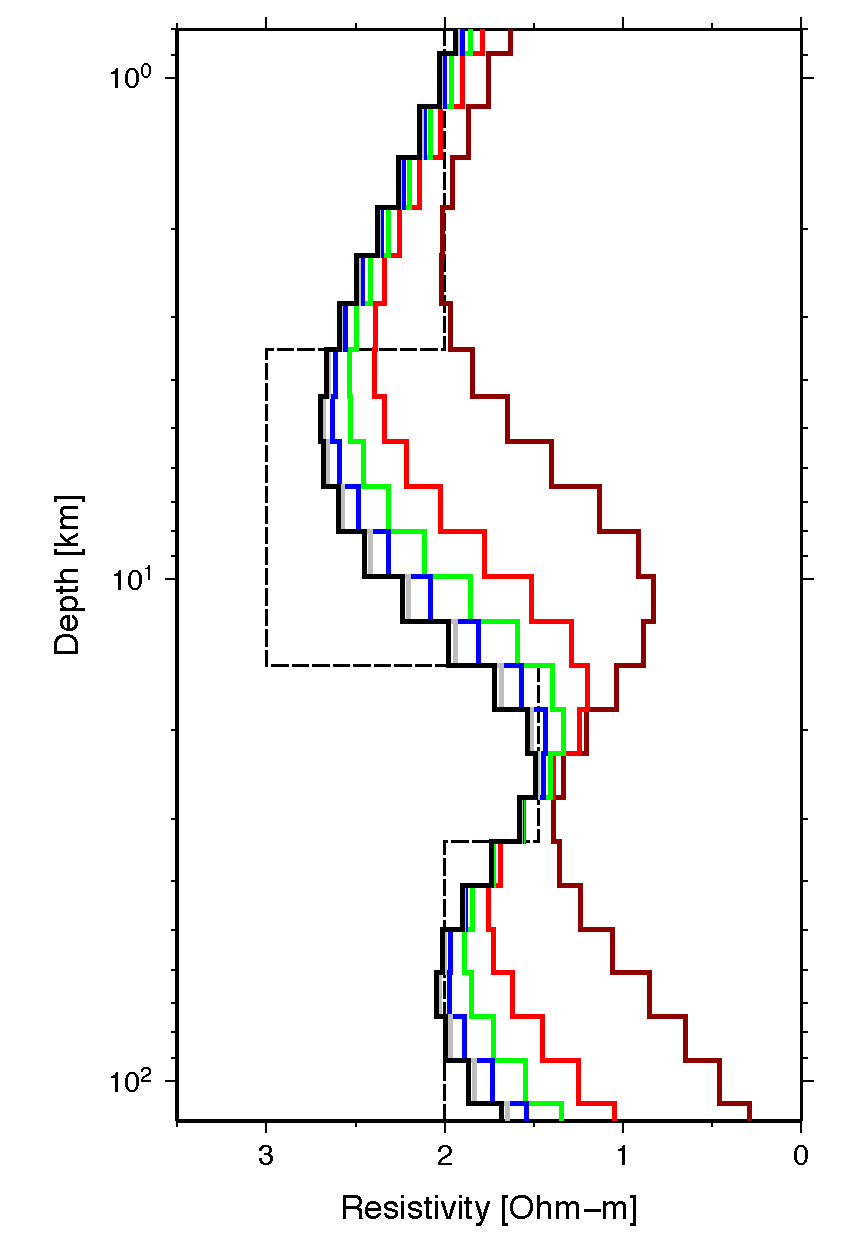
\includegraphics[scale=\plotinvmodelscale]{\figdir/lyr11a_n25_d13a_distorted-sdxa_site_dispse_det_inv1d.pdf}
		\label{fig:resp1d_avg_distorted_model_det}
	}
	\subfigure[]{
		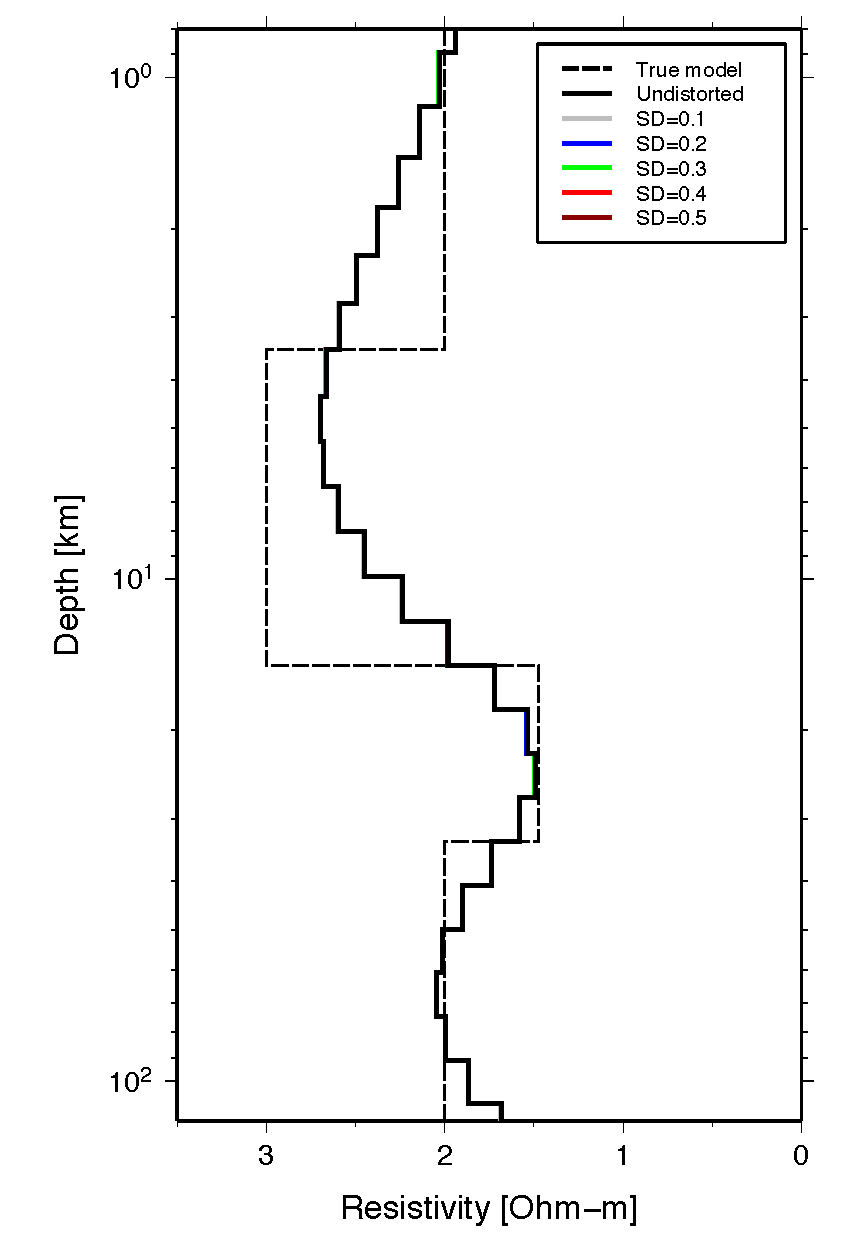
\includegraphics[scale=\plotinvmodelscale]{\figdir/lyr11a_n25_d13a_distorted-sdxa_site_dispse_ssq_inv1d.pdf}
		\label{fig:resp1d_avg_distorted_model_ssq}
	}
	\caption[Inverted models from average det and ssq impedances from distorted 1D datasets]{1D models obtained by inverting the average (a) det and (b) ssq impedances from the distorted 1D datasets (Figure \ref{fig:resp1d_avg_distorted}). The true structure (dashed lines) is also shown for comparison.}
	\label{fig:resp1d_avg_distorted_model}
\end{figure}


\clearpage

% !TEX root = ../../phdthesis_tawatr.tex 
\renewcommand{\thisdir}{_content/reg1d_synthetic_3d}
\renewcommand{\figdir}{\thisdir/_fig}

%% ==== ==== ==== ====
\section[3D examples]{Estimating a model of regional mean 1D profile: 3D example}\label{sect:example_3d}

%% ==== Model 3D plane view
\begin{figure}[!b]
	\centering
	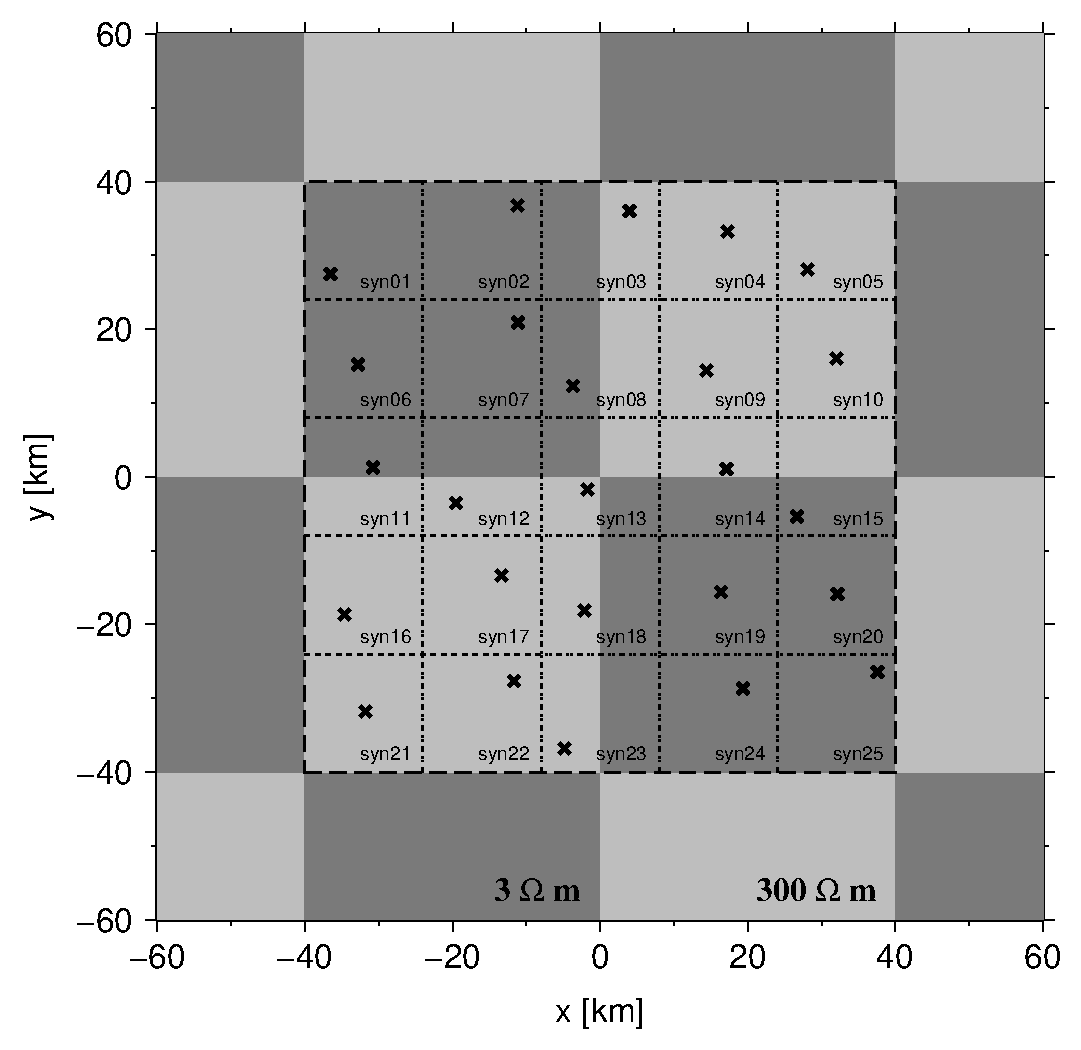
\includegraphics[width=\plotchkboardsize]{\figdir/m02a_chkboard12_h0a2a_s40k_p0p0_pp1.pdf}
	\caption[Checkerboard model and MT array setting used in this study]{Model of checkerboard anomalies with resistivities of 3 and 300 {\Ohmm} and a size of  \areakm{40}{40} embedded in the lower crust layer. The array of 25 irregularly distributed MT stations (crosses) covers the area of interest, which is {\areakm{80}{80}} (dashed frame). Here, one MT station represents an area of {\areakm{16}{16}} (dash-dotted frames).}
	\label{fig:model3d_setting}
\end{figure}

%% ==== 
The 3D model used in this work are generated from embedding checkerboard anomalies with resistivities of 3 and 300 {\Ohmm} and a size of \areakm{40}{40} (Figure \ref{fig:model3d_setting}) in the lower crust (14.8--33.3 km depth) of the layered-Earth model as in the 1D example (Figure \ref{fig:lyrearth_model}). The anomalies at this depth range could be detectable within the given period range.
% 
We can determine the inductive scale length using Eq. \eqref{eq:idl_anomaly}, where the conductivity contrast $\delta \sigma$ is $1/3 - 1/300$ Sm$^{-1}$. From the shortest to the longest periods (1--1,000 s), the inductive scale lengths corresponding to these anomalies range from 876 m to 27.7 km. They are not much smaller than its physical dimension (\areakm{40}{40}); therefore, the inductive effect from these anomalies should be sufficient.

%% ==== 
The details of the MT array configuration are as follows. The 25 MT stations are distributed over the area of interest which is \areakm{80}{80} (Figure \ref{fig:model3d_setting}). Consequently, the site spacing is 16 km, i.e., each site represents an area of \areakm{16}{16} (1/25 of the area of interest). To simulate the irregularly distributed MT array, the location of the $i$th station is given by
\begin{equation*}
	\begin{split}
		x_i & = x_c + s r_x \\
		y_i & = y_c + s r_y, \\
	\end{split}
\end{equation*}
where $(x_c,y_c)$ is the coordinate of the mesh center represented by each MT site; $s$ is the site spacing, which is 16 km in the setup; $r_x$ and $r_y$ are uniform random numbers bounded within $(-0.5,+0.5)$.

%% ==== Figure: 3D response individual all (undistorted)
\begin{figure}[!b]
	\centering
	\subfigure[]{
		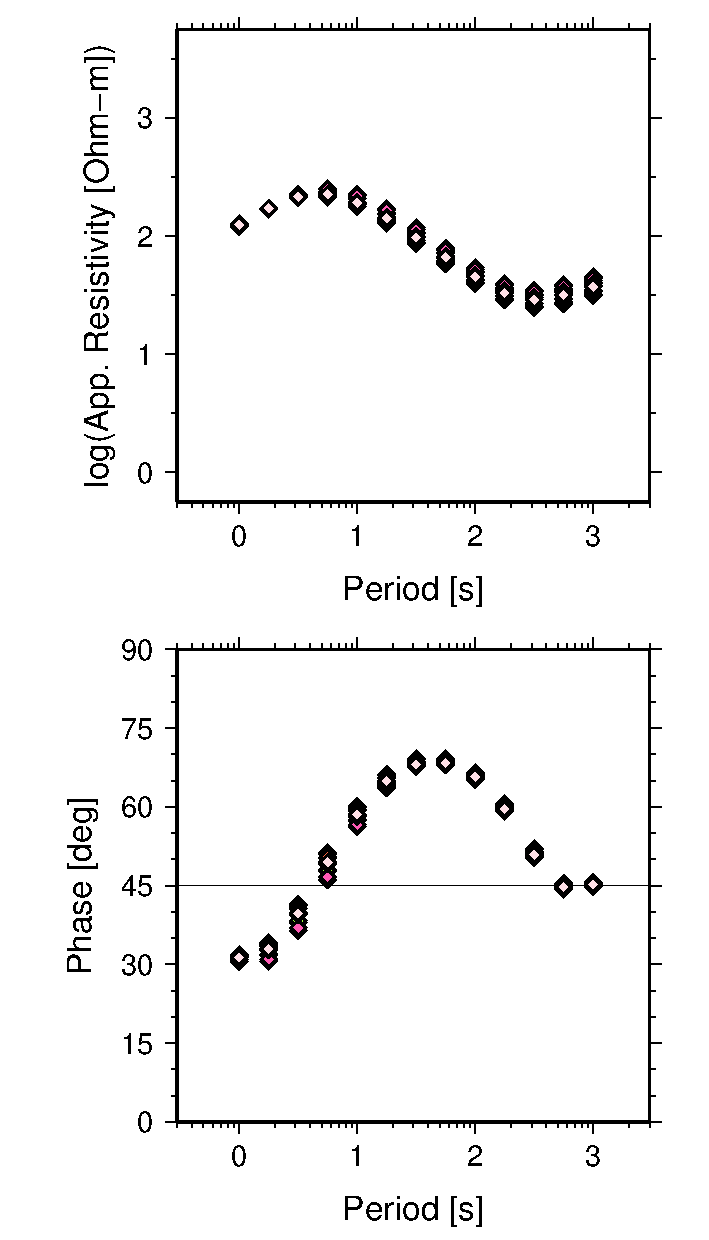
\includegraphics[scale=\plotmtrespscale]{\figdir/m02a-lyr11a_cb12-h0a2a-d05a-t01a_dr-e43n42_cb1X_loc-regi0_c-s40k-p0p0-pp1_d13a_undistorted_zinv_det_arsphs.pdf}
		\label{fig:resp3d_individual_all_undistorted_det}
	}
	\subfigure[]{
		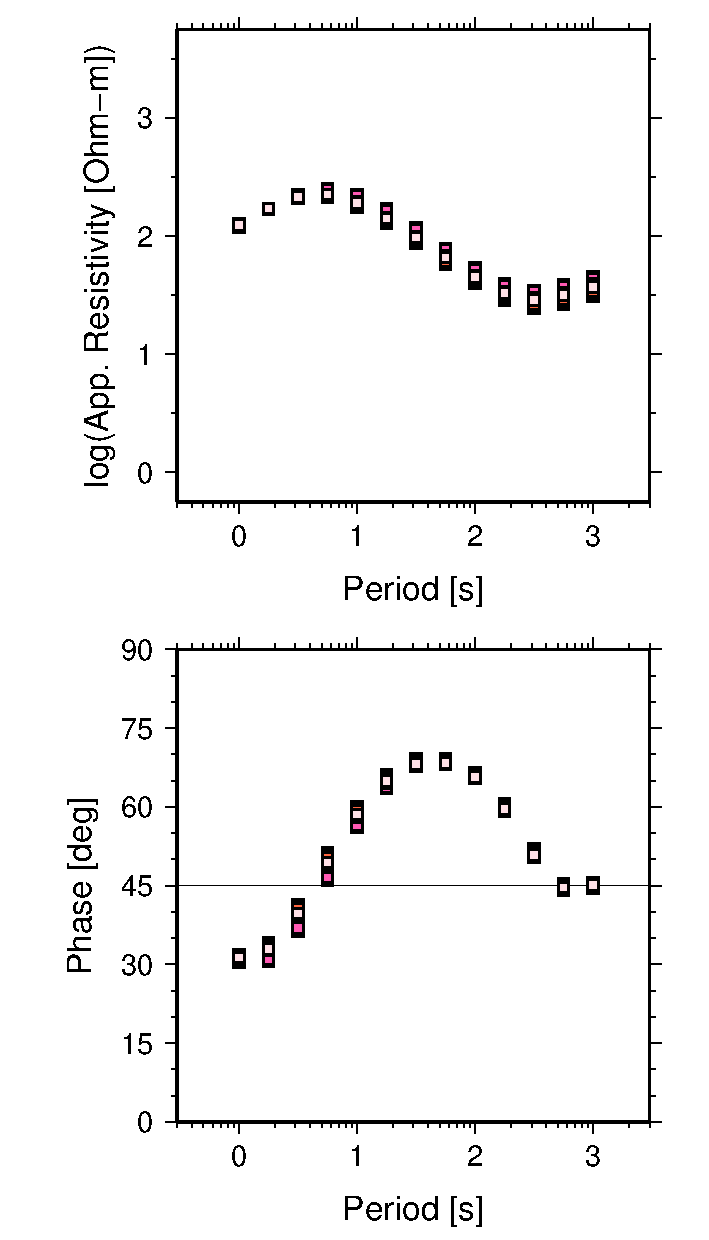
\includegraphics[scale=\plotmtrespscale]{\figdir/m02a-lyr11a_cb12-h0a2a-d05a-t01a_dr-e43n42_cb1X_loc-regi0_c-s40k-p0p0-pp1_d13a_undistorted_zinv_ssq_arsphs.pdf}
		\label{fig:resp3d_individual_all_undistorted_ssq}
	}
	\caption[Det and ssq impedances from MT array over the checkerboard model]{(a) Det and (b) ssq impedances from the array of MT stations over the 3D anomalies. Each station is represented by a different symbol color.}
	\label{fig:resp3d_individual_all_undistorted}
\end{figure}


%% ==== 
The MT responses are calculated using the software WSINV3DMT \citep{siripunvaraporn2005a}.  
%
Without galvanic distortion, the static shift is not observed in the det and ssq impedances, and their distributions are also similar (Figure \ref{fig:resp3d_individual_all_undistorted}). 
%
The checkerboard anomalies are recognized in the period range of 2--30 s, as seen from the slight variation in the impedances. 
%
To obtain the distorted 3D dataset, the set of random distortion parameters as used in the 1D example were applied to the calculated 3D data using Eq. \eqref{eq:z_distorted}. 
%
The example of the undistorted MT impedance from the station \texttt{syn08} is shown in Figure \ref{fig:resp3d_example_zij_undistorted}. The magnitudes of the diagonal components -- $xx$ and $yy$ -- are rather weak.
When it is distorted, their magnitudes increase (Figure \ref{fig:resp3d_example_zij_distorted}), and
 the phase mixing, i.e., the frequency dependent feature of the $xx$ phase, can be observed.
%
Unlike the 1D case, the ssq impedance from the distorted impedances is not only shifted, but also contains a weak frequency dependence (Figure \ref{fig:resp3d_example_distorted_zinv}), which is better observed from the difference of the magnitude and phase between the distorted and undistorted rotational invariants (Figure \ref{fig:resp3d_example_distorted_zinvdiff}).
As shown before, the phase of det impedance is not altered by galvanic distortion (Figure \ref{fig:resp3d_example_distorted_zinvdiff}), but its magnitude is biased downward due to the shear and splitting parameters as with the det impedance from the distorted 1D data.


%% ==== Figure: Distored 3D response example
\begin{figure}[t]
	\centering
	\subfigure[]{
		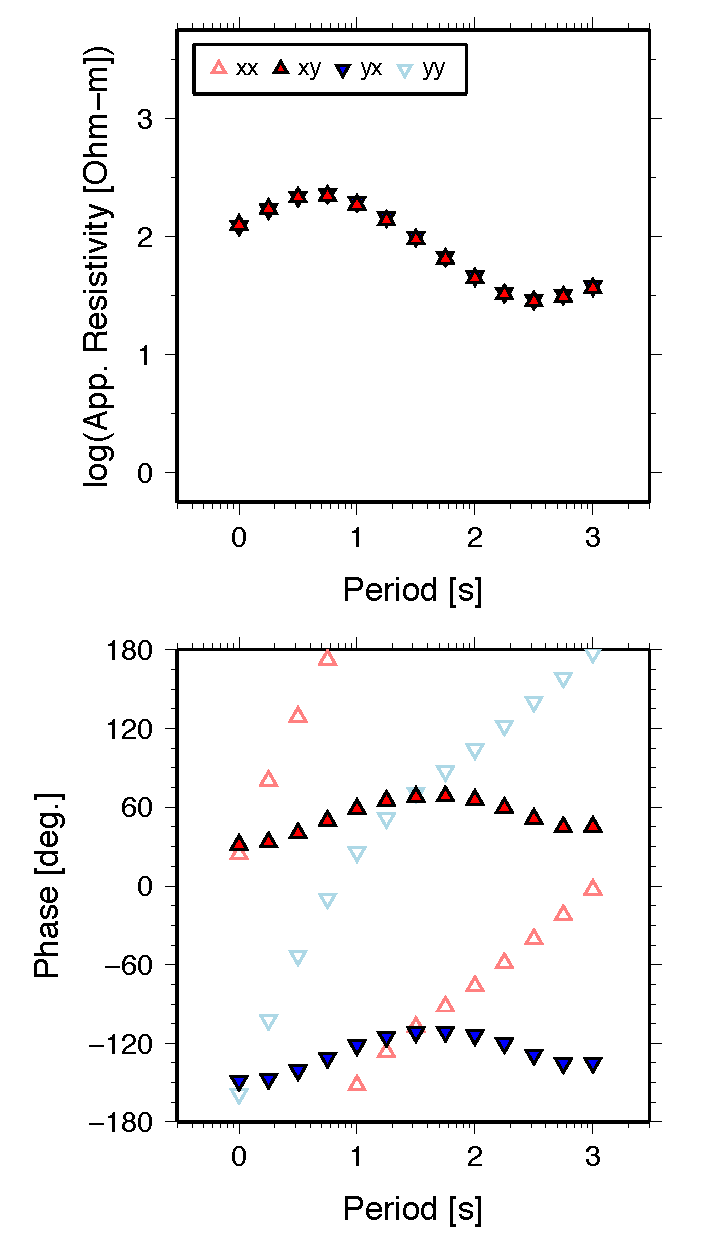
\includegraphics[scale=\plotmtrespscale]{\figdir/syni0203-azm000_zij_arsphs_undistorted.pdf}
		\label{fig:resp3d_example_zij_undistorted}
	}
	\subfigure[]{
		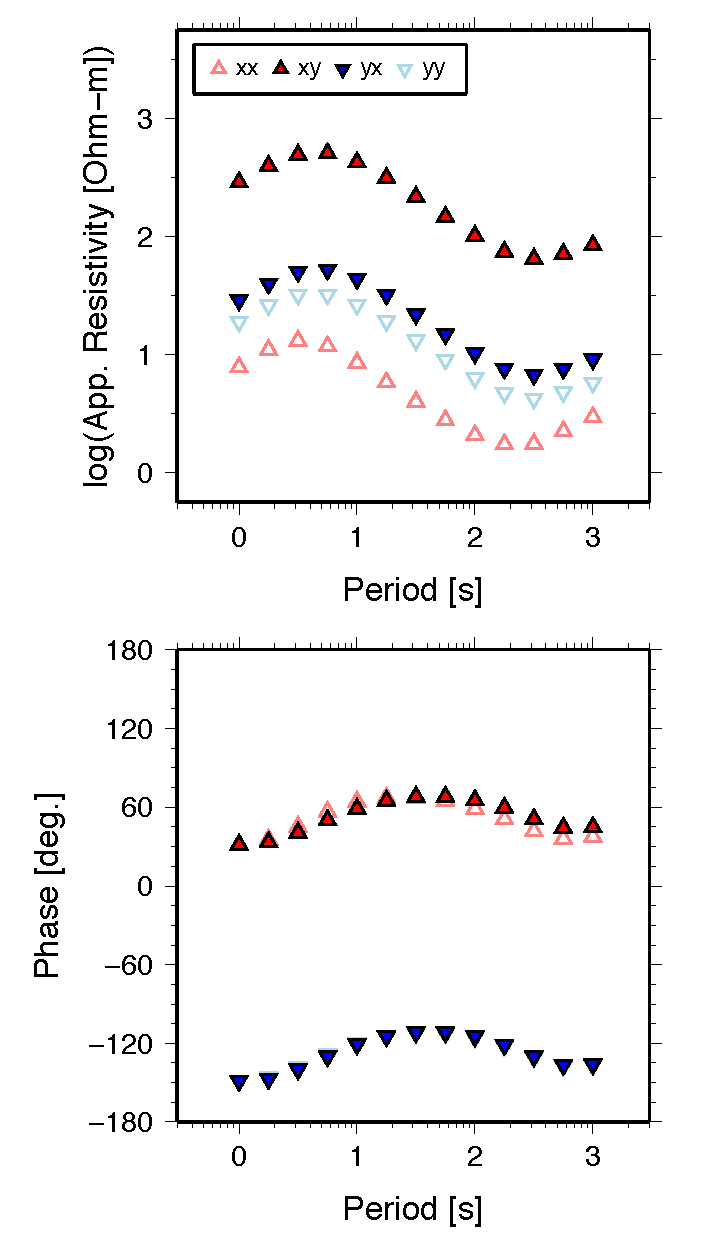
\includegraphics[scale=\plotmtrespscale]{\figdir/syni0203-azm000_zij_arsphs_distorted.pdf}
		\label{fig:resp3d_example_zij_distorted}
	}
	\caption[Examples of undistorted and distorted 3D MT data]{Components of the MT impedance from station \texttt{syn08} (a) undistorted and (b) distorted with $(g,t,e,s) = (1.20,0.11,-0.37,0.49)$.}
	\label{fig:resp3d_example_zij}
\end{figure}

%\redb{Individual from SD=0.3 and average}

As with the 1D example, the main feature observed from the det and ssq impedances due to the effect of random galvanic distortion paramters is an irregular shift (Figure \ref{fig:resp3d_individual_all_distorted_sd3a}). 
The advantage of using the ssq impedances is evident when they are averaged (Figure \ref{fig:resp3d_avg_distorted}). 
The error bar here is also the standard deviation.
As with the 1D example, the average ssq impedances has a smaller error bar smaller than the average det impedances at the same strength of galvanic distortion. 
This supports the idea that the ssq impedance is less dispersed due to galvanic distortion. 
Also, the average det impedances is biased downward by the splitting and shear parameters.

%% ==== Figure: Distored 3D response example inv
\begin{figure}[t]
	\centering
	\subfigure[]{
		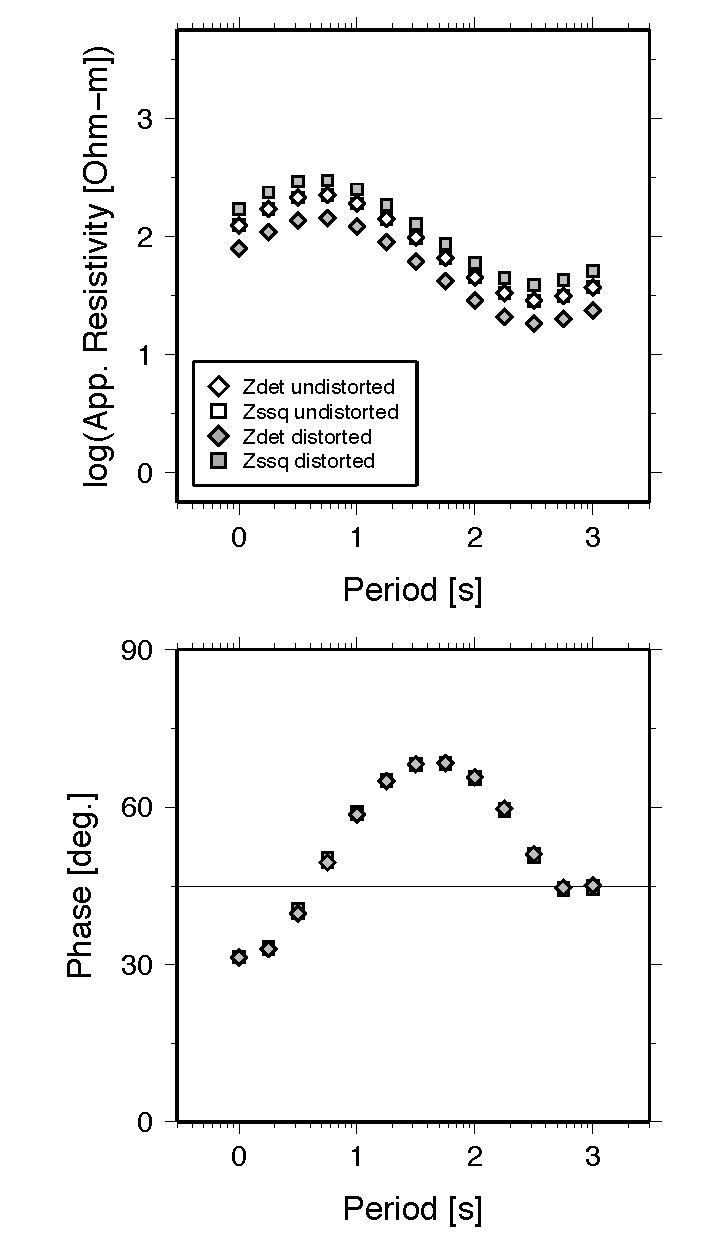
\includegraphics[scale=\plotmtrespscale]{\figdir/m02a-lyr11a_cb12-h0a2a-d05a-t01a_dr-e43n42_cb1X_loc-regi0_c-s40k-p0p0-pp1_d13a_syni0203_zinv_arsphs.pdf}
		\label{fig:resp3d_example_distorted_zinv}
	}
	\subfigure[]{
		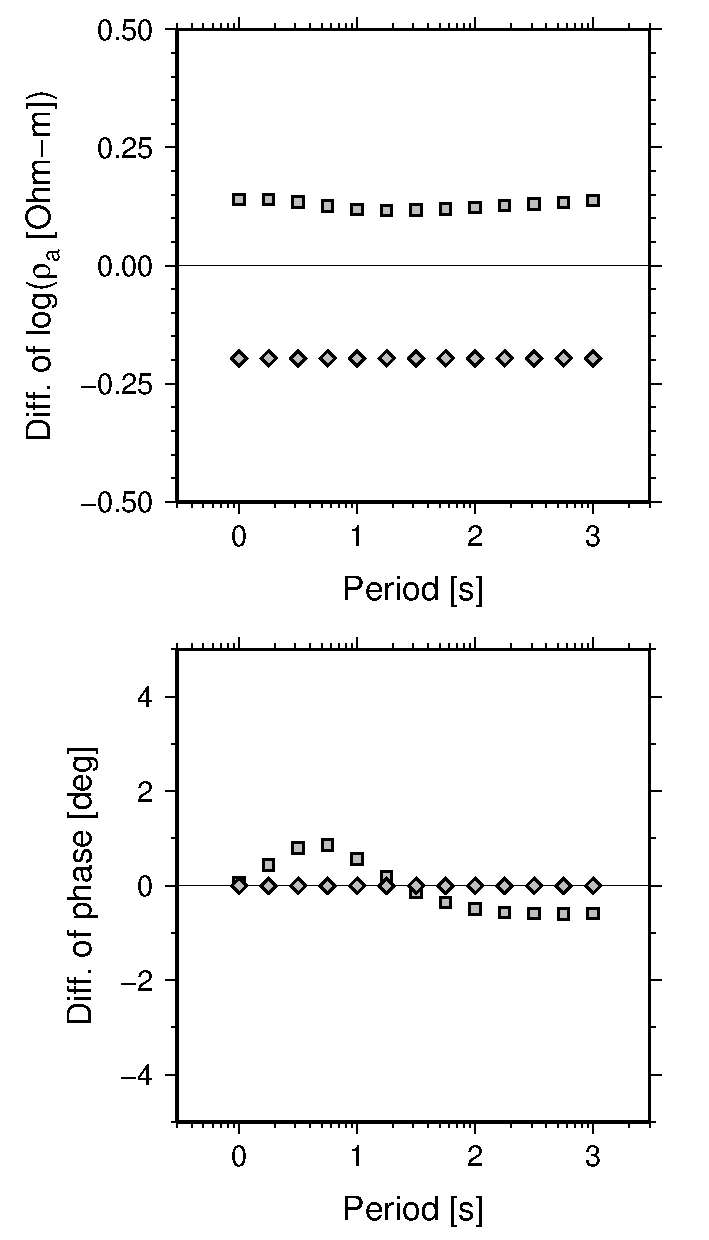
\includegraphics[scale=\plotmtrespscale]{\figdir/m02a-lyr11a_cb12-h0a2a-d05a-t01a_dr-e43n42_cb1X_loc-regi0_c-s40k-p0p0-pp1_d13a_syni0203_zinvdiff_arsphs.pdf}
		\label{fig:resp3d_example_distorted_zinvdiff}
	}
	\caption[Det and ssq impedances derived from the undistorted and distored MT impedance]{(a) Corresponding det and ssq impedances of the undistorted and distorted impedances in Figure \ref{fig:resp3d_example_zij}. (b) Difference between distorted and undistorted rotational invariant impedances.}
	\label{fig:resp3d_example_distorted}
\end{figure}

%\redb{Inverted model}

To yield the models of the regional mean 1D conductivity profile, the average distorted det and ssq impedances are inverted with the same uncertainty and convergence condition as used in the 1D example.
%
Without galvanic distortion, the average det and ssq impedances results in very similar models (Figure \ref{fig:resp3d_avg_distorted_model}).
The models estimated from the undistorted data both det and ssq impedances seem consistent with the theoretical models, which is obtanied by applying Eqs. \eqref{eq:regional_mean_linear} and \eqref{eq:regional_mean_log} to the conductivity distribution within the area of interest (dashed frame in Figure \ref{fig:model3d_setting}).
The discussion of the theoretical model is given in Section \ref{sect:reg1d_exam}.
%
As with the 1D example, when the galvanic distortion is included, the average det impedances will give the more conductive models of the regional mean 1D conductivity profile. On the contrary, using the average ssq impedances results in the models that are close to the model derived from the undistorted cases at any galvanic distortion strength.
This result strongly supports the idea that the average ssq impedance is an promising parameter in estimating the model of the regional mean 1D conductivity profile.





%% ==== Model 3D inverted individual
%\begin{figure}
%	\centering
%	\includegraphics[height=4in]{path1}
%	\caption{caption1}
%	\label{fig:caption1}
%\end{figure}


%\missingfigure[figwidth=6cm]{Figure showing 1D inverted from station over different underlying structure}



%% ==== Figure: Distored 3D response individual all
\begin{figure}[t]
	\centering
	\subfigure[]{
		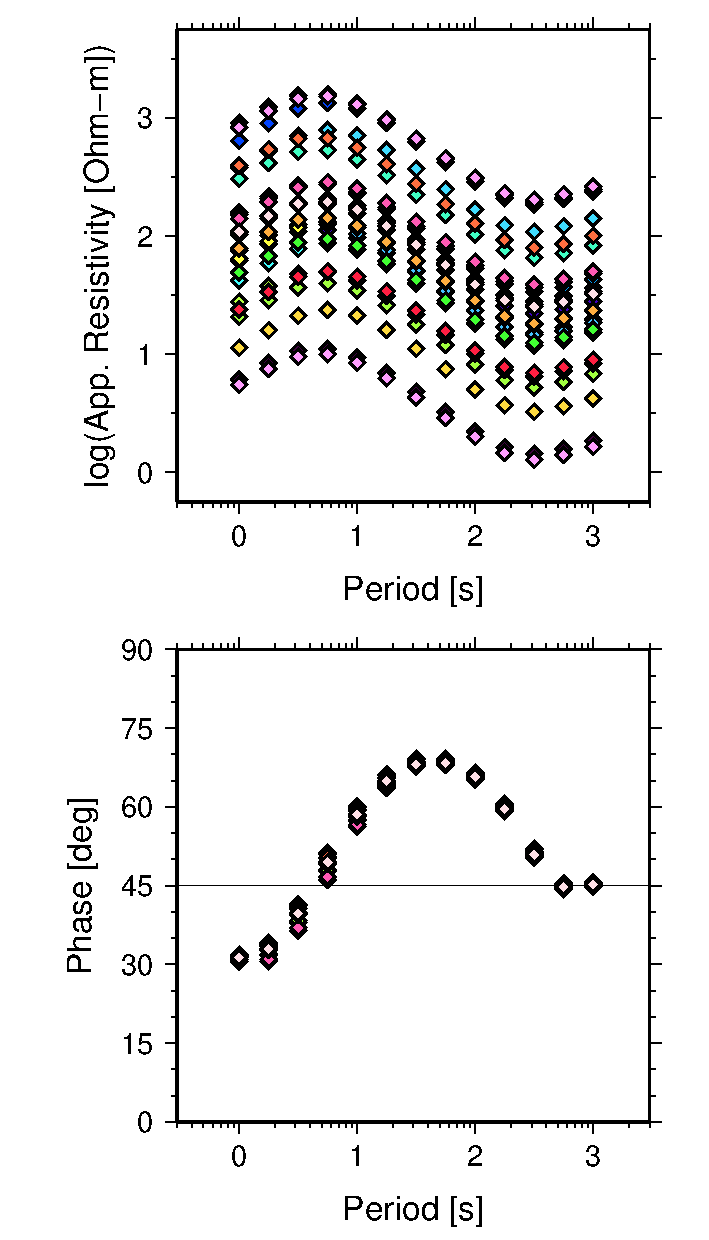
\includegraphics[scale=\plotmtrespscale]{\figdir/m02a-lyr11a_cb12-h0a2a-d05a-t01a_dr-e43n42_cb1X_loc-regi0_c-s40k-p0p0-pp1_d13a_distorted-sd3a-gtes_zinv_det_arsphs.pdf}
		\label{fig:resp3d_individual_all_distorted_sd3a_det}
	}
	\subfigure[]{
		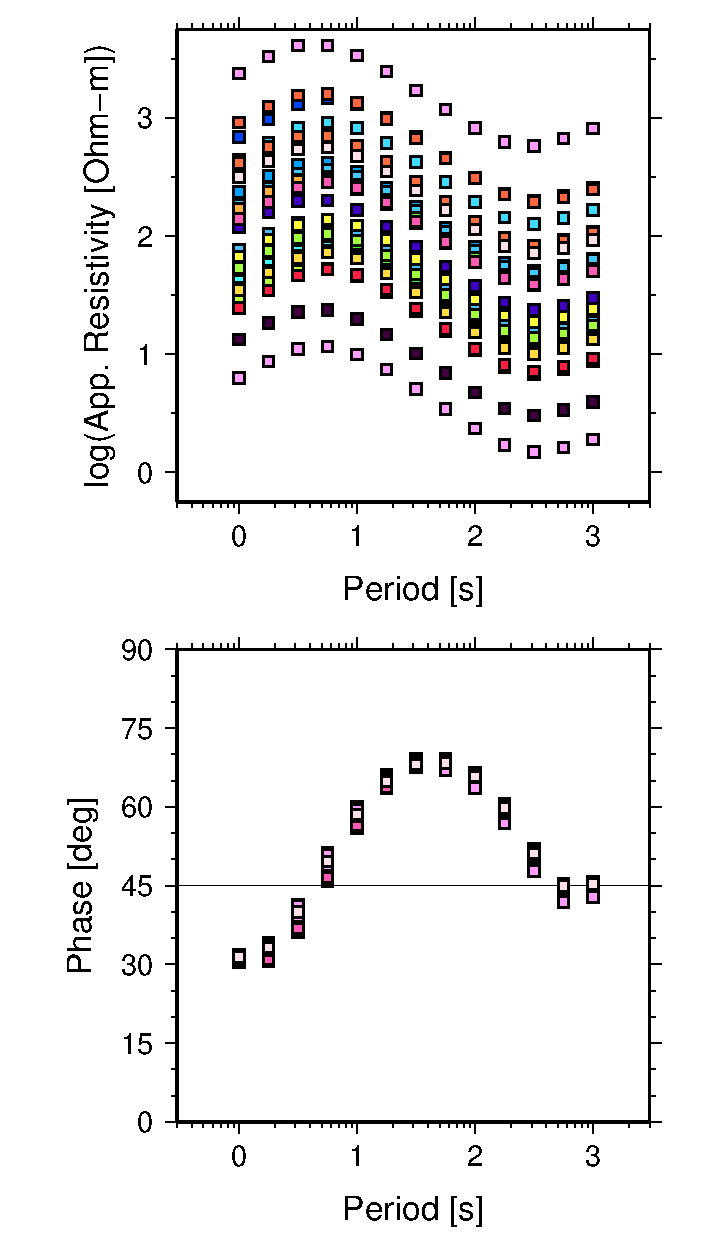
\includegraphics[scale=\plotmtrespscale]{\figdir/m02a-lyr11a_cb12-h0a2a-d05a-t01a_dr-e43n42_cb1X_loc-regi0_c-s40k-p0p0-pp1_d13a_distorted-sd3a-gtes_zinv_ssq_arsphs.pdf}
		\label{fig:resp3d_individual_all_distorted_sd3a_ssq}
	}
	\caption[Example of distorted det and ssq impedances from distorted 3D MTdataset]{(a) Det and (b) ssq impedances from the 3D example (as shown in Figures \ref{fig:resp3d_individual_all_undistorted_det} and \ref{fig:resp3d_individual_all_undistorted_ssq}, respectively) where a set of distortion parameters with an SD of 0.3 was applied.}
	\label{fig:resp3d_individual_all_distorted_sd3a}
\end{figure}

%% ==== Figure: Distored 3D response average
\begin{figure}[t]
	\centering
	\subfigure[]{
		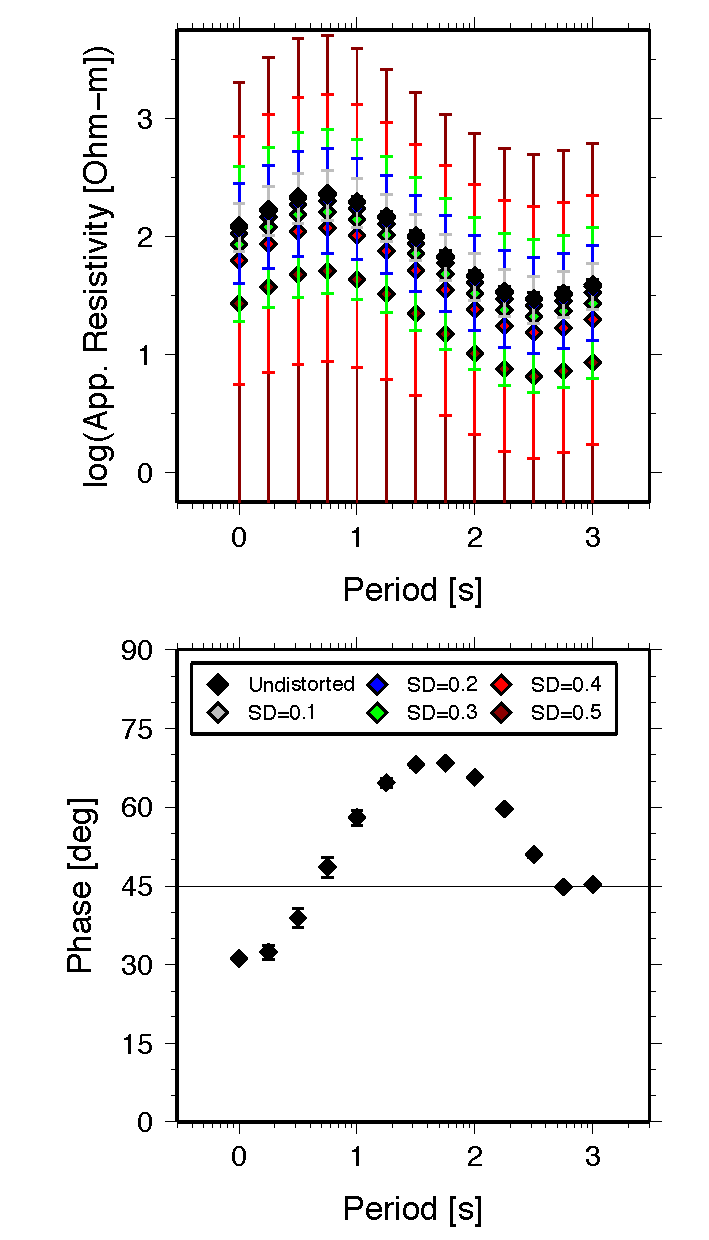
\includegraphics[scale=\plotmtrespscale]{\figdir/m02a-lyr11a_cb12-h0a2a-d05a-t01a_dr-e43n42_cb1X_loc-regi0_c-s40k-p0p0-pp1_d13a_distorted-sdxa_site_dispsd_zinv_det_arsphs.pdf}
		\label{fig:resp3d_avg_distorted_det}
	}
%	\hspace{1cm}
	\subfigure[]{
		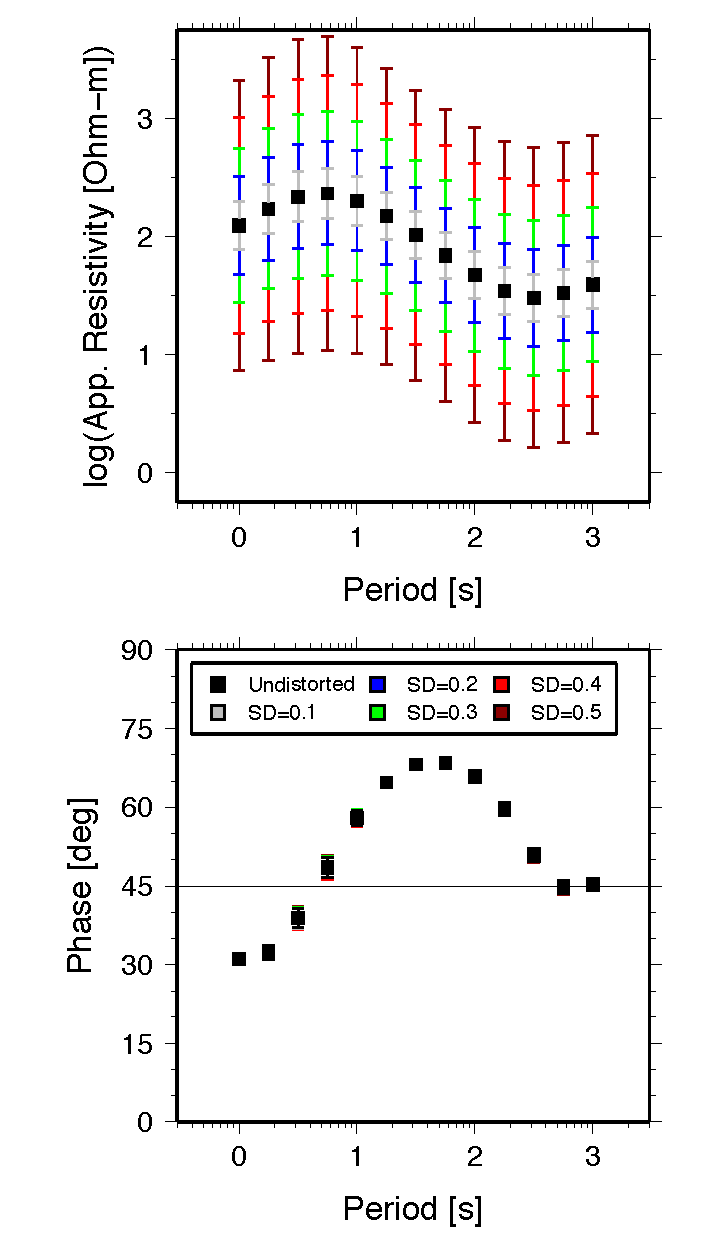
\includegraphics[scale=\plotmtrespscale]{\figdir/m02a-lyr11a_cb12-h0a2a-d05a-t01a_dr-e43n42_cb1X_loc-regi0_c-s40k-p0p0-pp1_d13a_distorted-sdxa_site_dispsd_zinv_ssq_arsphs.pdf}
		\label{fig:resp3d_avg_distorted_ssq}
	}
	\caption[Average det and ssq impedances from 3D MT datasets distorted
with different galvanic distortion strengths]{Average (a) det and (b) ssq impedances from the 3D datasets distorted with different galvanic distortion strengths.}
	\label{fig:resp3d_avg_distorted}
\end{figure}

%% ==== Figure: Distored 3D response average inverted
\begin{figure}[t]
	\centering
	\subfigure[]{
		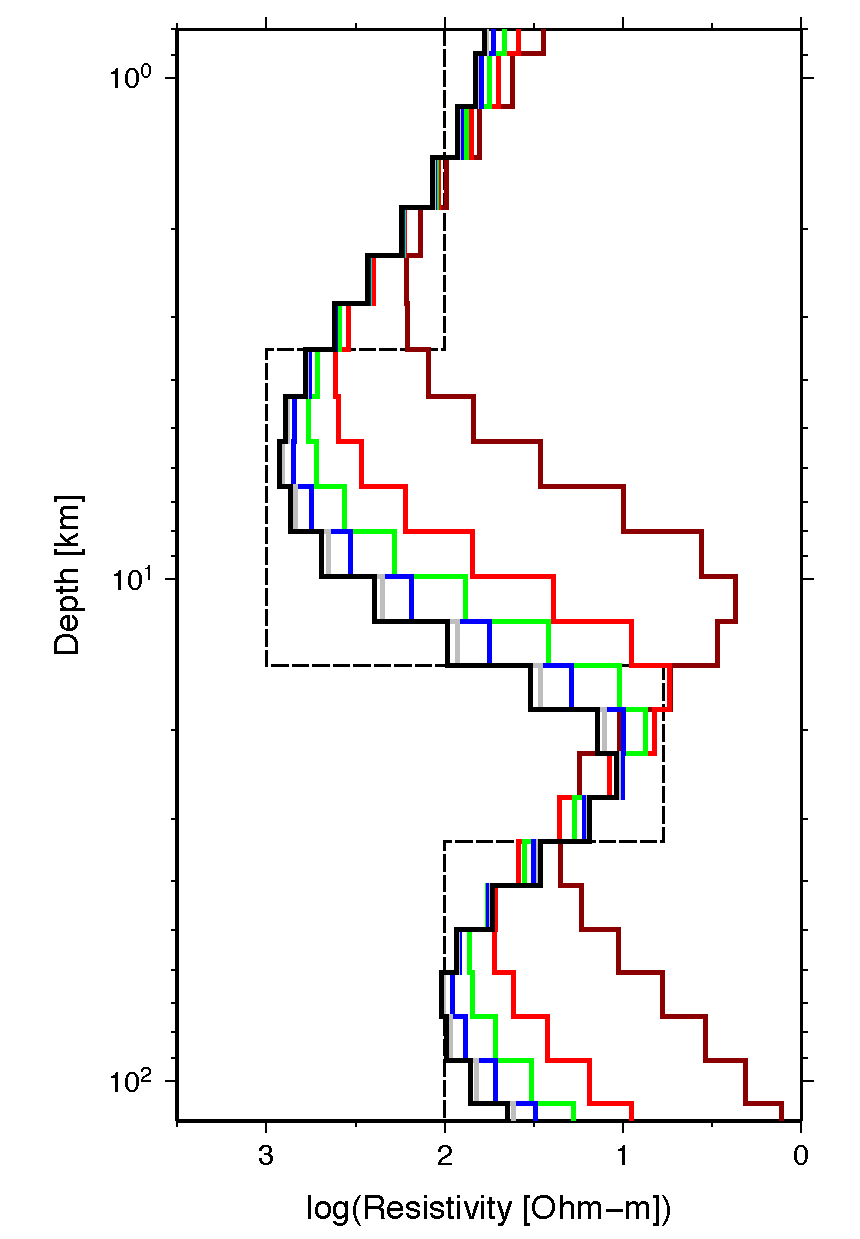
\includegraphics[scale=\plotinvmodelscale]{\figdir/m02a-lyr11a_cb12-h0a2a-d05a-t01a_dr-e43n42_cb1X_loc-regi0_c-s40k-p0p0-pp1_d13a_distorted-sdxa_site_dispse_det.pdf}
		\label{fig:resp3d_avg_distorted_model_det}
	}
	\subfigure[]{
		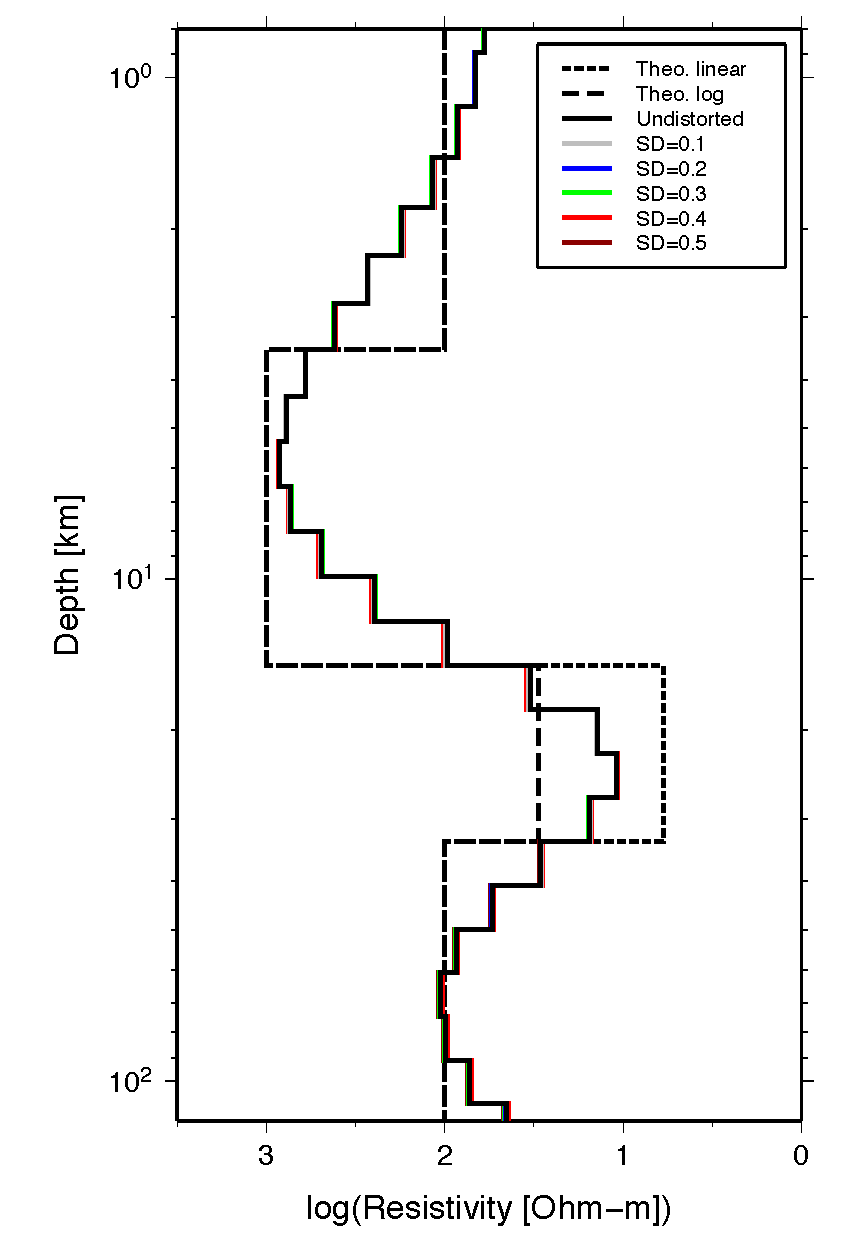
\includegraphics[scale=\plotinvmodelscale]{\figdir/m02a-lyr11a_cb12-h0a2a-d05a-t01a_dr-e43n42_cb1X_loc-regi0_c-s40k-p0p0-pp1_d13a_distorted-sdxa_site_dispse_ssq.pdf}
		\label{fig:resp3d_avg_distorted_model_ssq}
	}
	\caption[Inverted models from average det and ssq impedances from distorted 3D datasets]{1D models inverted from the average (a) det and (b) ssq impedances from the distorted 3D datasets (Figure \ref{fig:resp3d_avg_distorted}). The theoretical model of the mean 1D profile from this setting is shown for comparison.}
	\label{fig:resp3d_avg_distorted_model}
\end{figure}


\clearpage

% !TEX root = ../../phdthesis_tawatr.tex 
\renewcommand{\thisdir}{_content/reg1d_exam}
\renewcommand{\figdir}{\thisdir/_fig}

\section[Examination of theoretical definition]{Consistency examination of the theoretical model of regional mean 1D conductivity profile}\label{sect:reg1d_exam}

%% Introductory paragraph
%\begin{itemize}
%	\item 
	In analogy to the fact that the host layer Earth is absolutely unknown in reality, we proposed to compare the estimated model of the regional mean 1D conductivity profile with the theorectical model of the regional mean 1D conductivity profile instead of comparing it with the true layer Earth (e.g., the model in Figure \ref{fig:lyrearth_model}) in synthetic tests.
%	\item 
	In this section, we examined the consistency of the proposed theoretical model (Eqs. \ref{eq:regional_mean_linear} and \ref{eq:regional_mean_log}) and the estimated model of regional mean 1D conductivity profile with synthetic examples.
%\end{itemize}

%% ==== ==== Go to the content
In conducting MT surveys and other geophysical methods, 
a number of observations are made to sufficiently cover the target structure with the typical site spacing to resolve the smallest scale target.
%
This concept is analogous to the sampling theorem. 
%
To demonstrate the effect of the array size, in this consistency test, we test the array size that is larger than and comparable to the anomaly size at different locations.


% ==== ====
We used the 3D models and the array setup (25 MT stations within an area of \areakm{80}{80}) as used in Section \ref{sect:example_3d}. In this setup, the cluster is significantly larger than the anomaly.
We put the cluster in the three different locations: central, northwest and northeast positions (Figure \ref{fig:model3d_setting_pp1}). 
%
At the center, the array is concentric with the anomaly, while at the northeast and northwest locations, the arrays are, respectively, dominated by the 300 and 3 \Ohmm\ anomalies. In this case, three clusters contain the same portion of conductive and resistive anomalies.

%% ==== checkerborad, cluster 80 x 80
\begin{figure}[!t]
	\centering
	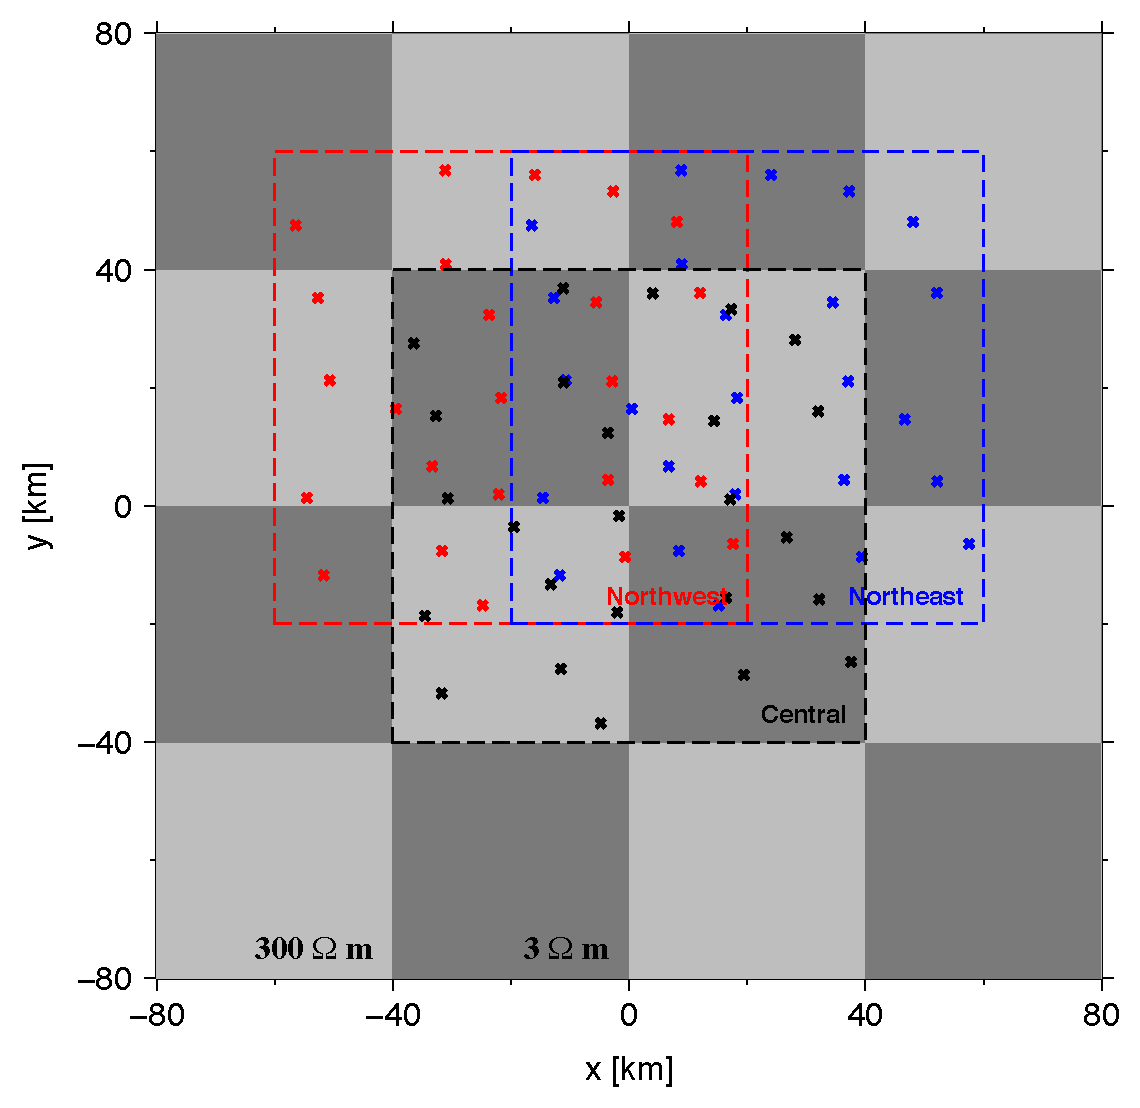
\includegraphics[width=\plotchkboardsize]{\figdir/m02a_chkboard12_h0a2a_s40k_pxpx_pp1.pdf}
	\caption[MT array, in which its size is comparable to the anomaly size, located at different position]{Checkerboard model with an anomaly size of {\areakm{40}{40}} and resistivities of 3 (dark gray) and 300 (light gray) {\Ohmm}. The checkerboard anomaly was embedded in the lower crust layer. Three arrays of 25 MT stations (crosses) each with a size of {\areakm{80}{80}}  (dashed frames) were placed at the central (black), northeast (blue), and northwest (red) positions.}
	\label{fig:model3d_setting_pp1}
\end{figure}
%% ==== checkerborad, cluster 80x80 results
\begin{figure}[!h]
	\centering
	\subfigure[]{
		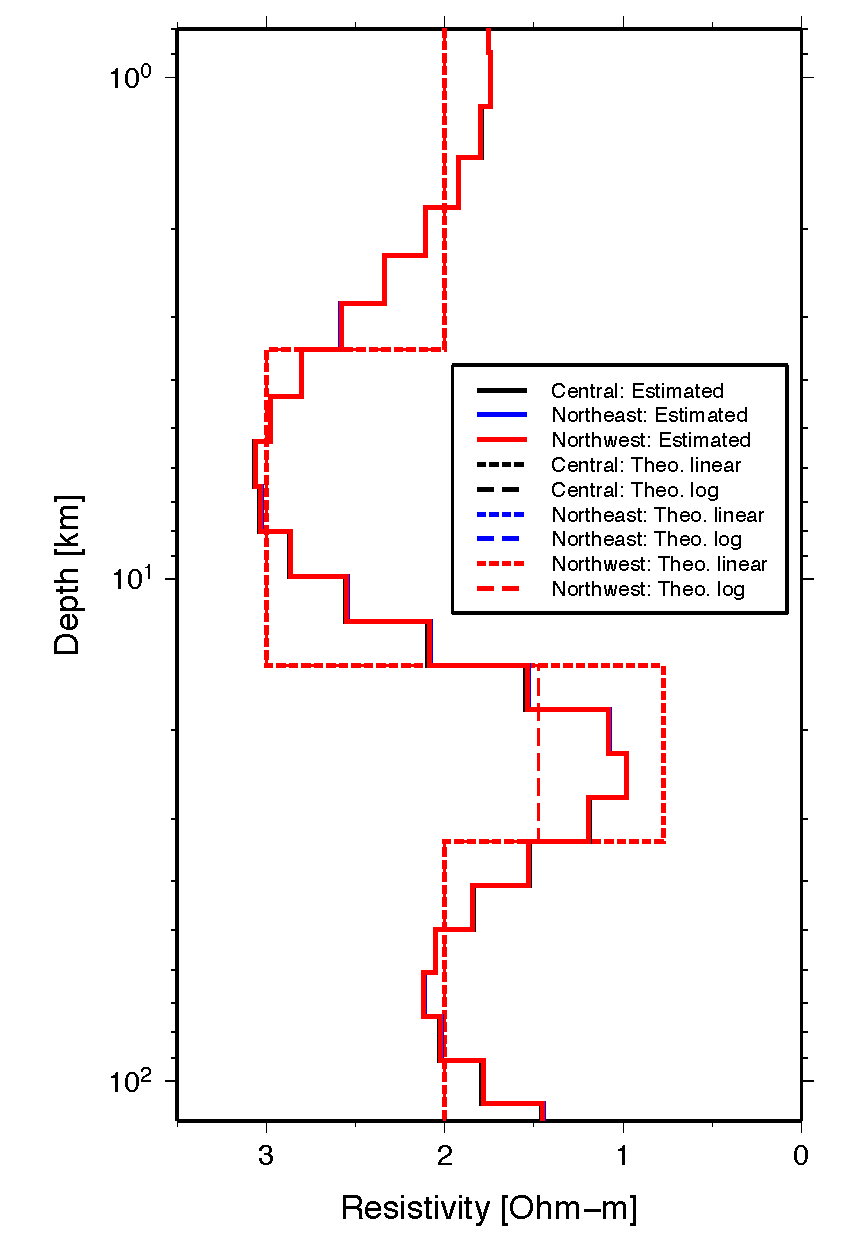
\includegraphics[scale=\plotinvmodelscale]{\figdir/m02a_lyr11a_chkboard12-h0a2a-d05a-t01a_chkboard1X_s40k_pxpx_pp1_d13a_ssq_r2.pdf}
		\label{fig:cb_resp_pxpx_pp1_model}
	}
	\subfigure[]{
		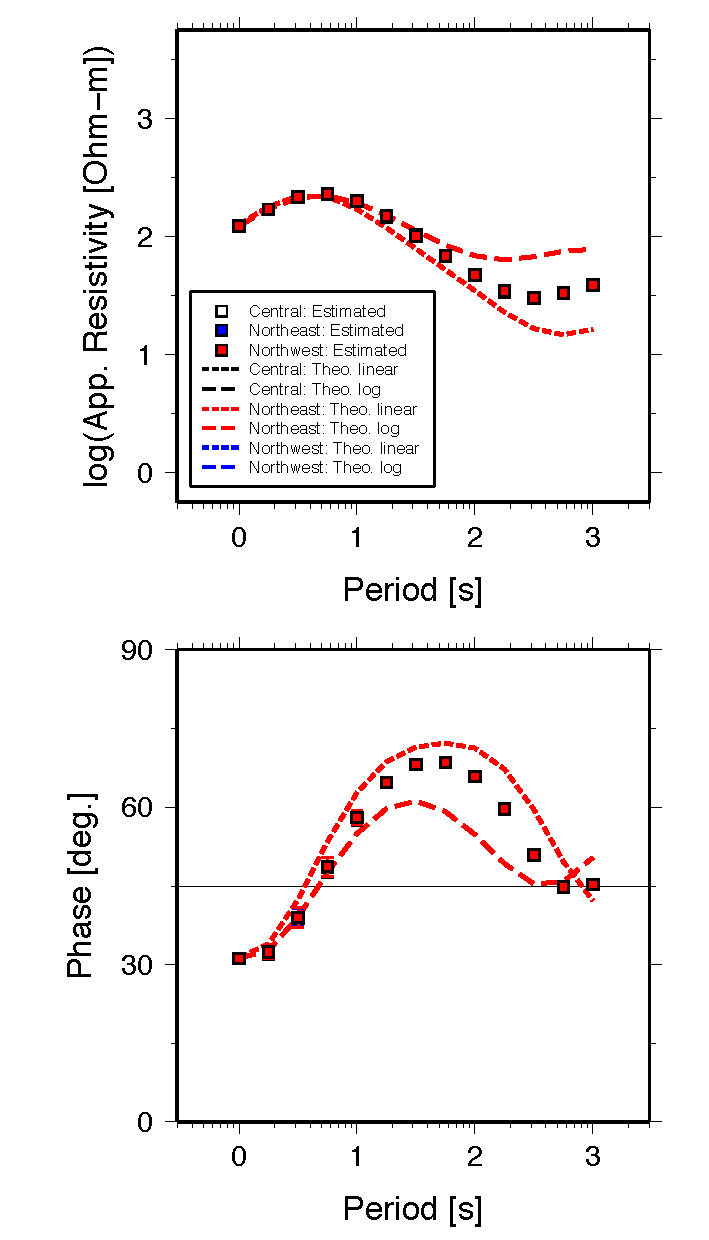
\includegraphics[scale=\plotmtrespscale]{\figdir/m02a_lyr11a_chkboard12-h0a2a-d05a-t01a_chkboard1X_s40k_pxpx_pp1_d13a_ssq_arsphs.pdf}
		\label{fig:cb_resp_pxpx_pp1_resp}
	}
	\caption[Theoretical and estimated model of regional mean 1D profile from large MT arrays]{(a) Theoretical (dashed lines) and estimated (solid lines) models of the mean 1D profiles obtained using the settings shown in Figure \ref{fig:model3d_setting_pp1}. (b) Corresponding MT responses from the theoretical (dashed line) and estimated (squares) models of the mean 1D profiles. The results obtained from different array locations are represented by lines and symbols of different colors.}
	\label{fig:cb_resp_pxpx_pp1}
\end{figure}

% ==== ====
The estimated models of the regional mean 1D conductivity profiles from these clusters were calculated from the average ssq impedance. Note that only the ssq impedance is used in this section, because the galvanic distortion is not of concern. 
%
The theoretical models of the regional mean 1D conductivity profile were calculated using the given definitions from the conductivity in the clusters (e.g., dashed frames in Figure \ref{fig:model3d_setting_pp1}), and
the MT responses from the theoretical models were then obtained using the analytic solution \citep{constable1987a}.

% ==== ==== Large array
%\redb{-- Large array --}

%\begin{itemize}
%	\item
When the arrays are larger than the anomaly, the arrays contain the comparable portions of the resistive and conductive heterogeneities, even though they are at different locations.
The estimated and theoretical models of the regional mean 1D conductivity profiles from different clusters are likely identical (Figure \ref{fig:cb_resp_pxpx_pp1}). 
In other words, the average approach is spatially independent for the large array. Hence, the average approach is a robust method to obtain the regional mean 1D conductivity profile.
%	\item
The smooth and step shapes of the estimated and theoretical models might be due to the smoothness constraint applied in the inversion.
%\end{itemize}




%% ==== ==== Small array.
%\redb{-- Small array --}

%\begin{itemize}
%	\item
Next, we demonstrate how array size affects the models of the regional mean 1D conductivity profile by decreasing the array size to \areakm{40}{40} (Figure \ref{fig:model3d_setting_pp0}), which is equal to the anomaly size. The cluster locations were kept the same as in the previous test.


%	\item
	In this case, the theoretical models from different cluster locations are totally different (Figure \ref{fig:cb_resp_pxpx_pp0_model}) because 
the clusters occupy different portions of resistive and conductive anomalies.
The northwest cluster covers only the underlying 3 {\Ohmm} anomaly, for example.
Note that when the array resides on the layered-Earth like structure, e.g., the cluster on the northwest and northeast positions, the theoretical models from the log and the linear average definition are the same (Figure \ref{fig:cb_resp_pxpx_pp0_model}). 
	%
	In constrast to the theoretical models, the estimated models of regional mean 1D profile remain spatially independent in this setup. This is because the inductive effect from the anomalies is indistinguishable from different array locations.
%	\item 
	It is expected that if the anomaly is significantly large or the cluster is very small, the estimation method would show the spatially dependent feature.
%\end{itemize}

%% ==== ==== Difference between the linear and log average
%\redb{-- Difference between the linear and log average --}

%\begin{itemize}
%	\item
	 As expected, using the logarithmic average definition (Eq. \ref{eq:regional_mean_log}) would give the less conductive structure (e.g., Figure \ref{fig:cb_resp_pxpx_pp1_model}). 
%	\item
	 Although, the theoretical models from the linear and log average definition are noticeably different (Figures \ref{fig:cb_resp_pxpx_pp1_model} and \ref{fig:cb_resp_pxpx_pp0_model}) when both conductive and resistive anomalied are contained in the array, they are both consistent with the estimated model. 
	Hence, both definitions are acceptable for calculating the theoretical model of the regional mean 1D conductivity profile.
%\end{itemize}

%% ==== ==== Describing the inconsistency
% \redb{-- Inconsistency --}
 
% \begin{itemize}
%	\item
	When the array is significantly larger than the anomaly, the estimation and the theoretical definition are rather consistent.
	But, when the array is comparable or smaller than the anomaly, the inconsistency is clearly observed, particularly, at the depth where the anomalies are embedded (Figure \ref{fig:cb_resp_pxpx_pp0}). 
%	\item 
	However, the inconsistency seems to be less evident when the cluster is located over the conductive anomaly (e.g., the northwest cluster), because of the nature of the electromagnetic induction that the conductive anomaly will produce significant inductive effect when compared to the resistive anomaly.
%	\item
	This inconsistency is a consequence of an inappropriate design of the observation array, e.g., the cluster is not sufficiently large to cover the anomaly. The tests also suggest that the estimation of the regional mean 1D profile would be reliable with a large size of array.
%\end{itemize}

%% ==== ==== Concluding paragraph
%\redb{-- Concluding paragraph --}

%\begin{itemize}	
%	\item 
	In general, the exact dimension of the target structure is unknown. One may be able to approximate its from other information such as geological background or past studies.
%	\item
	The observation array is then designed so as to cover the target structure.
%	\item 
	However, if the anomaly geometry is found to be comparable to the size of the array then the resulting conductivity image may be affected by the array location. One suggestion is to increase the array size by adding additional MT stations in order to get the reliable results.
%\end{itemize}

%\red{This synthetic example gives the instructive suggestion for the design of observation array according to the target structure.}

%% ==== ==== Figure



%% ==== checkerborad, cluster 40x40 
\begin{figure}[!h]
	\centering
	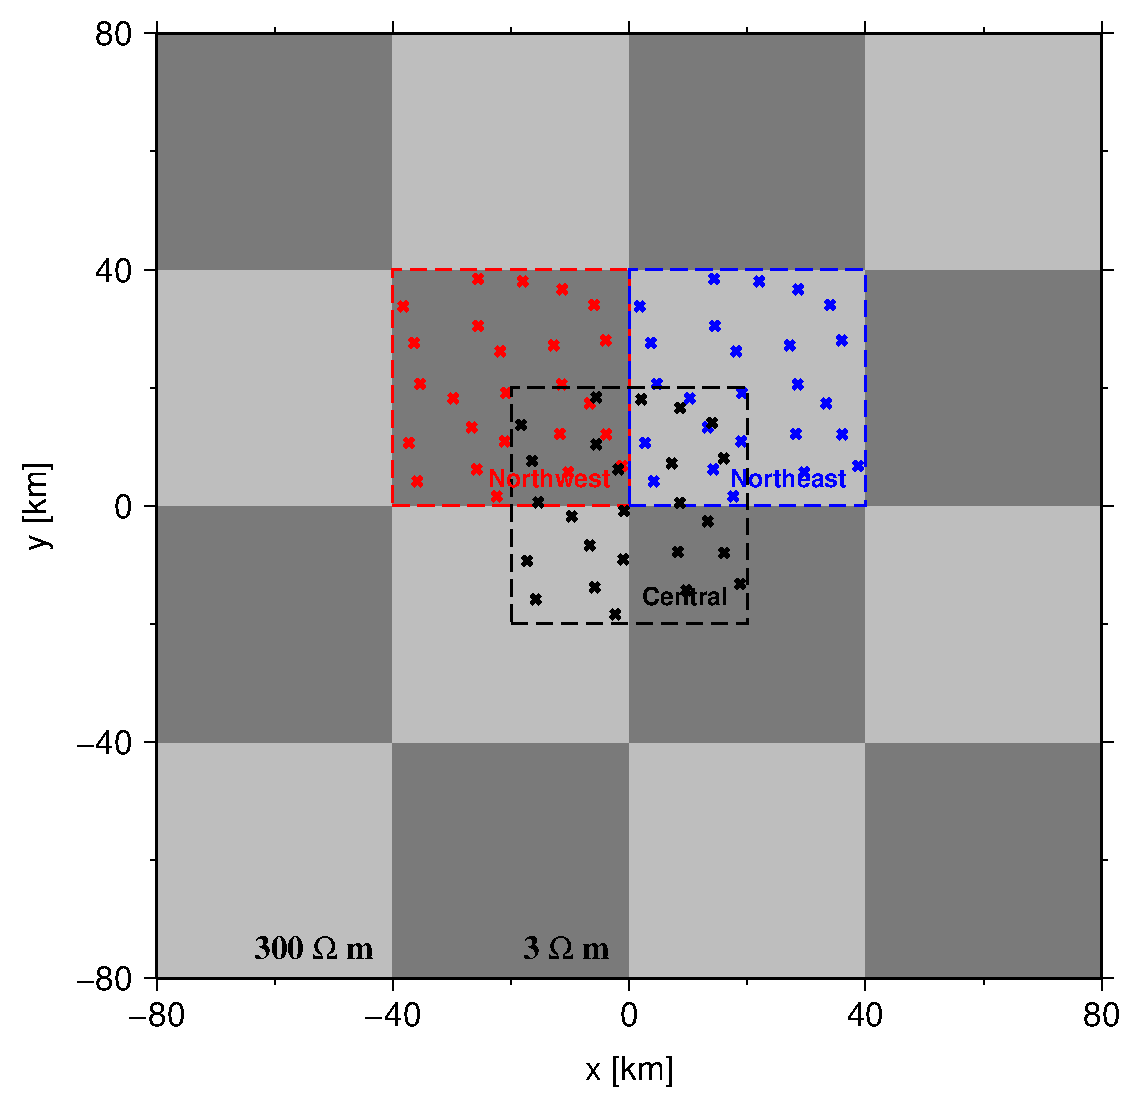
\includegraphics[width=\plotchkboardsize]{\figdir/m02a_chkboard12_h0a2a_s40k_pxpx_pp0.pdf}
	\caption[Same as Figure \ref{fig:cb_resp_pxpx_pp1} for small arrays]{Same as Figure \ref{fig:cb_resp_pxpx_pp1} for an array size of \areakm{40}{40}.}
	\label{fig:model3d_setting_pp0}
\end{figure}

%% ==== checkerborad, cluster 40x40 results
\begin{figure}[t]
	\centering
	\subfigure[]{
		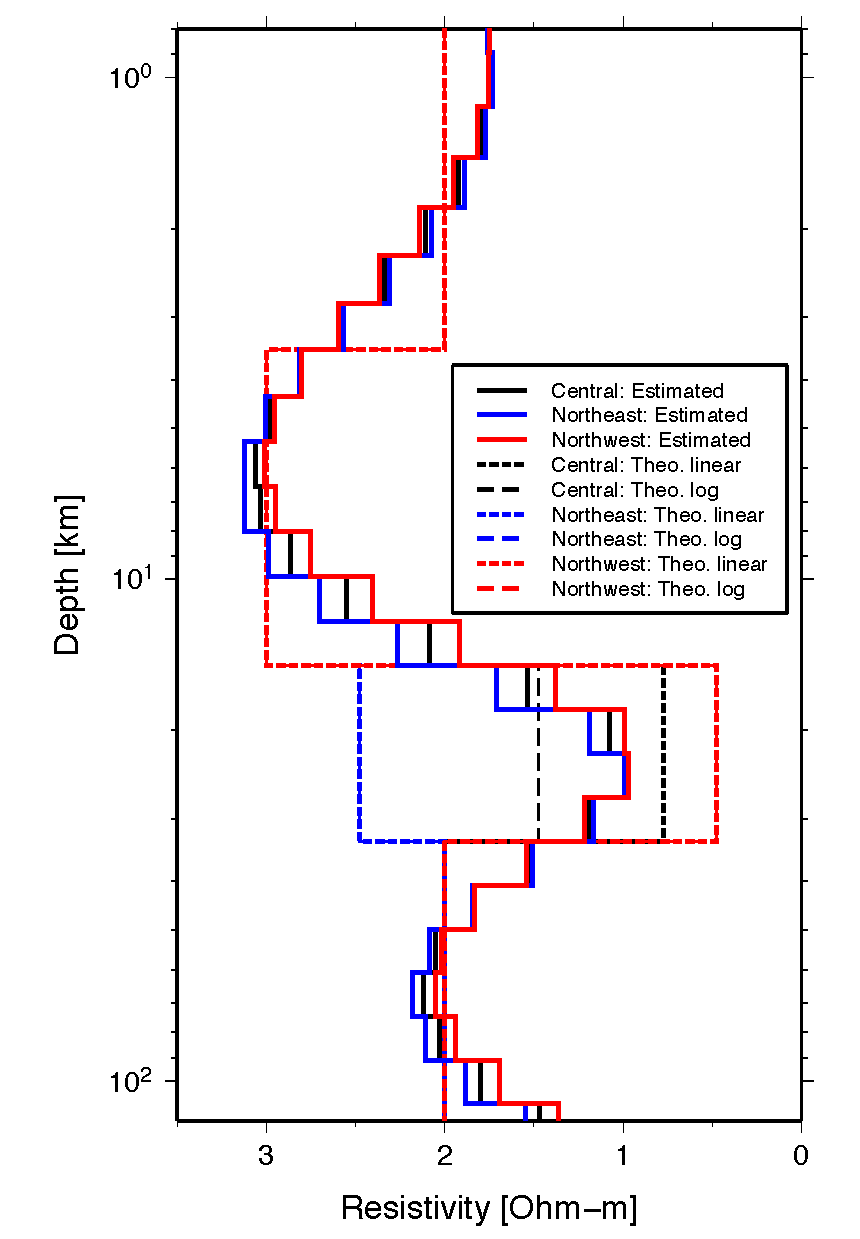
\includegraphics[scale=\plotinvmodelscale]{\figdir/m02a_lyr11a_chkboard12-h0a2a-d05a-t01a_chkboard1X_s40k_pxpx_pp0_d13a_ssq_r2.pdf}
		\label{fig:cb_resp_pxpx_pp0_model}
	}
	\subfigure[]{
		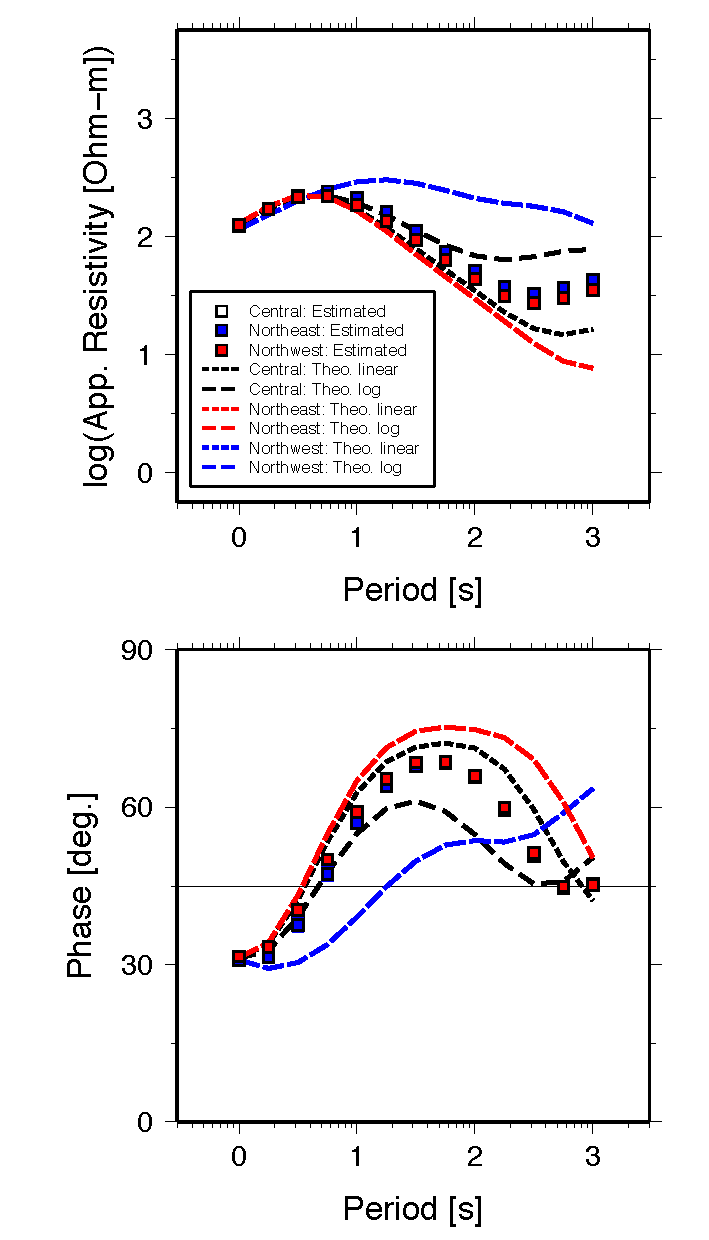
\includegraphics[scale=\plotmtrespscale]{\figdir/m02a_lyr11a_chkboard12-h0a2a-d05a-t01a_chkboard1X_s40k_pxpx_pp0_d13a_ssq_arsphs.pdf}
		\label{fig:cb_resp_pxpx_pp0_resp}
	}
	\caption{Same as Figure \ref{fig:cb_resp_pxpx_pp1} for the settings shown in Figure \ref{fig:model3d_setting_pp0}.}
	\label{fig:cb_resp_pxpx_pp0}
\end{figure}


\clearpage

% !TEX root = ../../phdthesis_tawatr.tex 
\renewcommand{\thisdir}{_content/gamma}
\renewcommand{\figdir}{\thisdir/_fig}
\section{Local and regional distortion indicators}

%% ==== Introductory paragraph
This section shows the example of local and regional distortion indicators (Eqs \ref{eq:gamma_local_def} and \ref{eq:gamma_regional_def}) derived from the synthetic 1D and 3D examples in Sections \ref{sect:example_1d} and \ref{sect:example_3d}, respectively.

%% ==== local 1D
%\begin{itemize}

%	\item 
	In this test, these local distortion indicators are obtained by applying Eq. \eqref{eq:gamma_local_def} to the det and ssq impedances from the 1D dataset distorted with the distortion parameter with an SD of 0.3 (as shown in Figure \ref{fig:resp1d_individual_all_distorted_sd3a}), for example.
%	\item 
	As shown earlier, the local distortion indicators derived from distorted 1D data are shifted upward (greater than unity) and remain real-valued.
%	\item 
	The local distortion indicators are shifted irregularly depending on the strength of shear and splitting parameters at individual sites (Figure \ref{fig:gamma_local_example_1d}). 
%	\item 
	In addition, the calculated local distortion indicator from the data distorted with $\gtes = (1.20,0.11,-0.37,0.49)$, for example, agrees well with the actual value (gray circles and dashed line in Figure \ref{fig:gamma_local_example_1d}, respectively).
	Note that the actual local distortion indicator is calculated by substituting the shear and splitting parameters of $-0.37$ and 0.49 into Eq. \eqref{eq:gamma_1d_analytic}.
%\end{itemize}

%% ==== local 3D
%\begin{itemize}
%	\item 
	For 3D cases, the local distortion indicators contain both the frequency dependent and independent features (Eq. \ref{eq:gamma_approx}). The frequency independent part is mainly due to the shear and splitting parameters, which are real-valued, while the frequency dependent part is ascribed by the difference between the ssq and det impedances at individual sites, which is complex-valued and rather weak in general.
%	\item 
	As with the 1D example, the example of local distortion indicators from distorted 3D data (Figure \ref{fig:gamma_regional_example_3d}) are also obtained by applying Eq. \eqref{eq:gamma_local_def} to the 3D data distorted with the distortion parameter with an SD of 0.3 (as shown in Figure \ref{fig:resp3d_individual_all_distorted_sd3a}).
	In contrast to the 1D case, the local distortion indicators from distorted 3D data show a frequency-dependent feature and become complex-valued, which depends on how strong the inductive effect from the underlying structure is and the galvanic distortion strength posed in the data. 
%	\item
	The local distortion indicator derived from the data at the station \texttt{syn08}, which is distorted by $\gtes$ of $(1.20,0.11,-0.37,0.49)$, are compared with the actual value of the local distortion indicators.
	Although the local distortion indicator is deviated because of the inductive effect of the underlying structure, it still oscillates about the actual values (gray circles and dashed line in Figure \ref{fig:gamma_local_example_3d}). Hence the local distortion indicator can be used to indicate the strength of shear and splitting effects.
%\end{itemize}

%% ==== Gamma local
\begin{figure}[t]
	\centering
	\subfigure[]{
		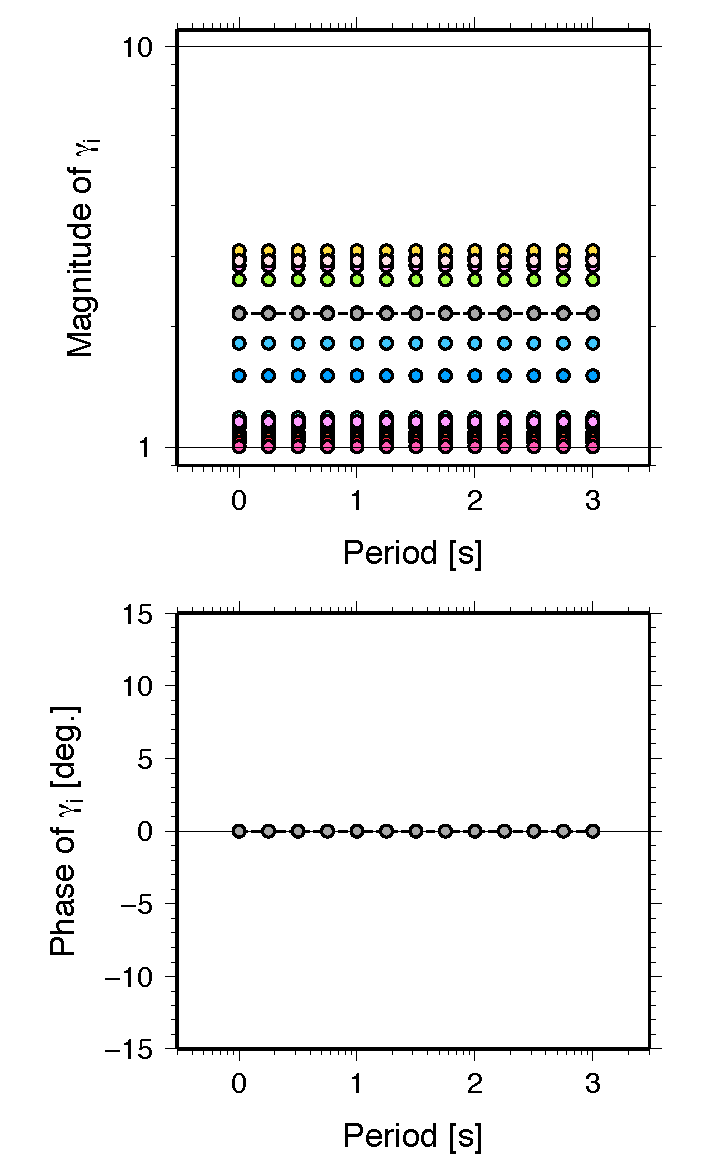
\includegraphics[scale=\plotmtrespscale]{\figdir/lyr11a_n25_d13a_distorted-sd3a-gtes_gamma_magphs_merged.pdf}
		\label{fig:gamma_local_example_1d}
	}
	\subfigure[]{
		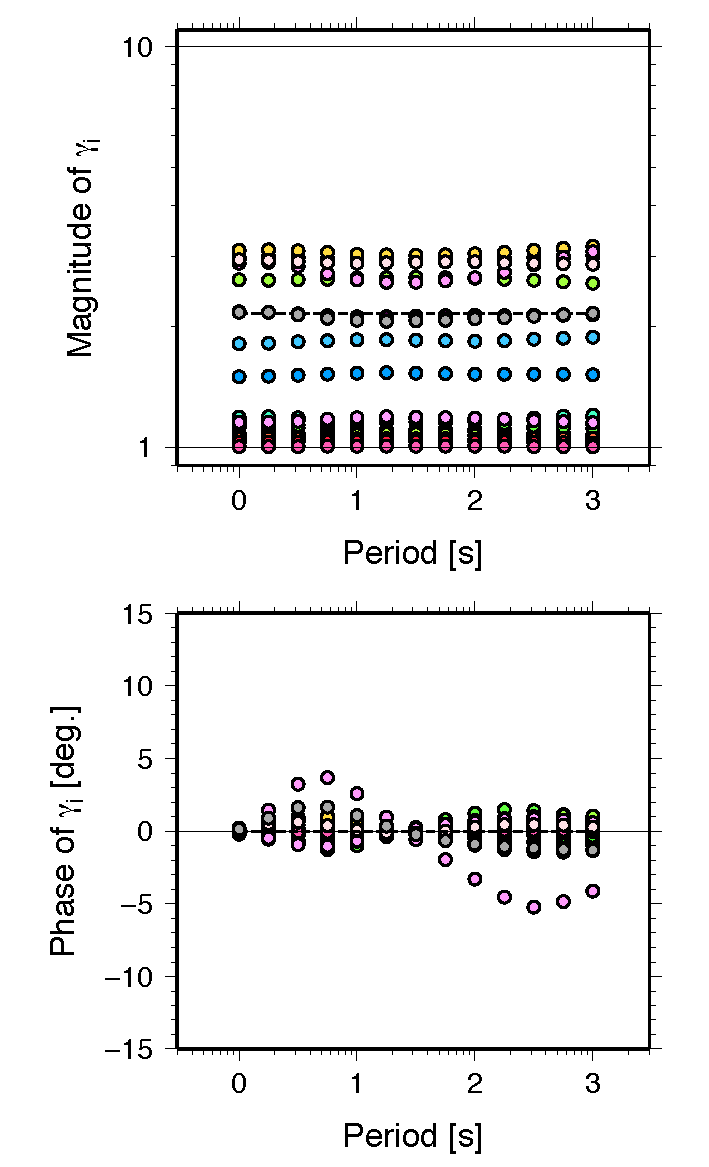
\includegraphics[scale=\plotmtrespscale]{\figdir/m02a-lyr11a_cb12-h0a2a-d05a-t01a_dr-e43n42_cb1X_loc-regi0_c-s40k-p0p0-pp1_d13a_distorted-sd3a-gtes_gamma_magphs_merged.pdf}
		\label{fig:gamma_local_example_3d}
	}
	\caption[Local distortion indicators from 1D and 3D data]{Local distortion indicators from the distorted (a) 1D and (b) 3D data (in Sections \ref{sect:example_1d} and \ref{sect:example_3d}, respectively) where a set of distortion parameters with an SD of 0.3 was applied. Examples of 1D and 3D data at station \texttt{syn08} distorted with $(g, t, e, s) = (1.20, 0.11, -0.37, 0.49)$ (gray circles) are compared with the actual values of the local distortion indicator at this station (dashed lines)}
	\label{fig:gamma_local_example}
\end{figure}

%%%% ==== Local exception
However, if the strong 3D effect (e.g., coastal effect) or the inductive distortion is contained, the local distortion indicator would become very frequency dependent and rather complex valued. In such a case, the treatment of distortion as galvanic orgin is not allowed. In other words, the local distortion indicator is able to indicate the period range where the data is inductively distorted as well as galvanically distorted. Thus the local distortion indicator will help judge the validity of applying phase tensor, because the phase tensor is defined for the case with the galvanic distortion only.





%%% ==== Local distortion indicator: Mean
The mean local distortion indicators $\gammaimean$ of the 1D and 3D dataset distorted with the set of distortion parameters with SD of 0.3 (Figures \ref{fig:gamma_1d_site} and \ref{fig:gamma_3d_site}) are calculated using Eq. \eqref{eq:gamma_local_mean_def}.
%
Compared to the local distortion indicators (Figures \ref{fig:gamma_local_example_1d} and \ref{fig:gamma_local_example_3d}), it is more convenient to identify the site-to-site strength of the shear and splitting effect.
%
They are shown in comparison with the actual local distortion indicators $\gammai$, which are calculated by substituting the synthetic shear and splitting parameters at each station into Eq. \eqref{eq:gamma_local_def}.
%
We also define the percentage difference between the mean local distortion indicator and the actual local distortion indicators for validation purposes:
	\begin{equation}
		\mathcal{P}(\gammaimean) = \frac{\gammaimean - \gammai}{\gammai} \times 100\%.
	\end{equation}	
In the 1D case, the mean local distortion indicator is able to correctly estimate the strength of galvanic distortion with zero difference (Figure \ref{fig:gamma_1d_site}).
%
As shown earlier, the underlying structure may affect the local distortion indicator in 3D case as a frequency dependent contribution.
%
Here, the error bar is set to the standard deviation in order to represent the dispersion of the frequency dependent part in the local distortion indicator. For example, the station \texttt{syn02} has the significant frequency-dependent variation.
Although some errors in estimating the galvanic distortion strength appear in the distorted 3D data (Figure \ref{fig:gamma_3d_site}), they are still in the acceptable range.

%% ==== The percentage difference of local distortion indicators 1-D
%\missingfigure[figwidth=6cm]{P. diff of local distortion indicators}
\begin{figure}[!t]
	\centering
	\subfigure[]{
		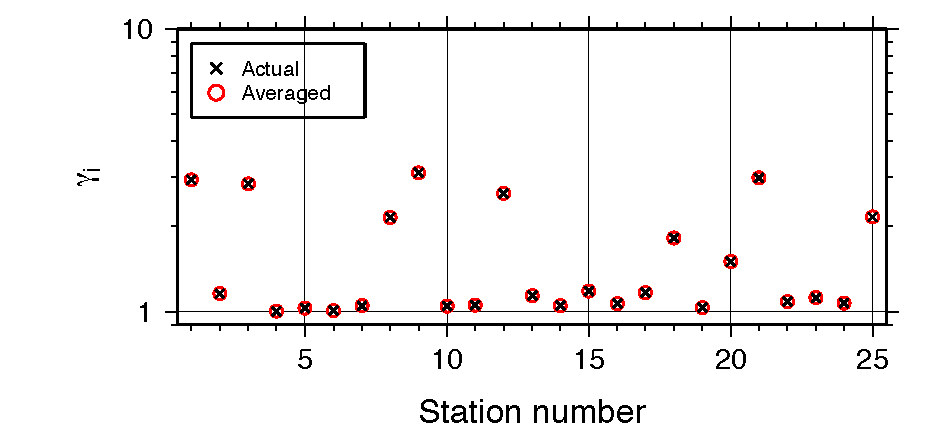
\includegraphics[scale=\plotdindmeanscale]{\figdir/lyr11a_n25_d13a_distorted-sd3a-gtes_gamma_est.pdf}
		\label{fig:gamma_1d_site_estimated}
	}
	\subfigure[]{
		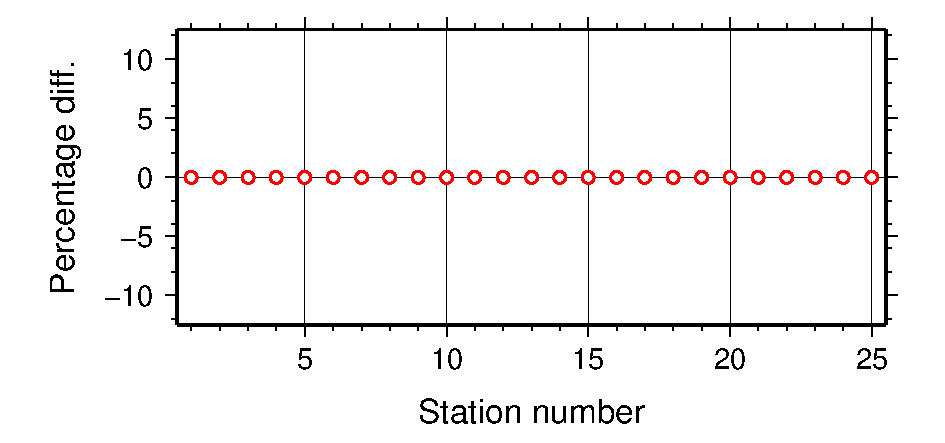
\includegraphics[scale=\plotdindmeanscale]{\figdir/lyr11a_n25_d13a_distorted-sd3a-gtes_gammapdiff.pdf}
		\label{fig:gamma_1d_site_pdiff}
	}
	\caption[Comparison of the actual and the mean local distortion indicators and percentage difference]{(a) Comparison of actual local distortion indicators (crosses) with the mean local distortion indicators (red circles) from the 1D example, where a set of distortion parameters with an SD of 0.3 was applied (Figure \ref{fig:resp1d_individual_all_distorted_sd3a}). (b) Percentage difference between the mean local distortion indicators and the actual ones.}
	\label{fig:gamma_1d_site}
\end{figure}
%% ==== The percentage difference of local distortion indicators 3-D
\begin{figure}[t]
	\centering
	\subfigure[]{
		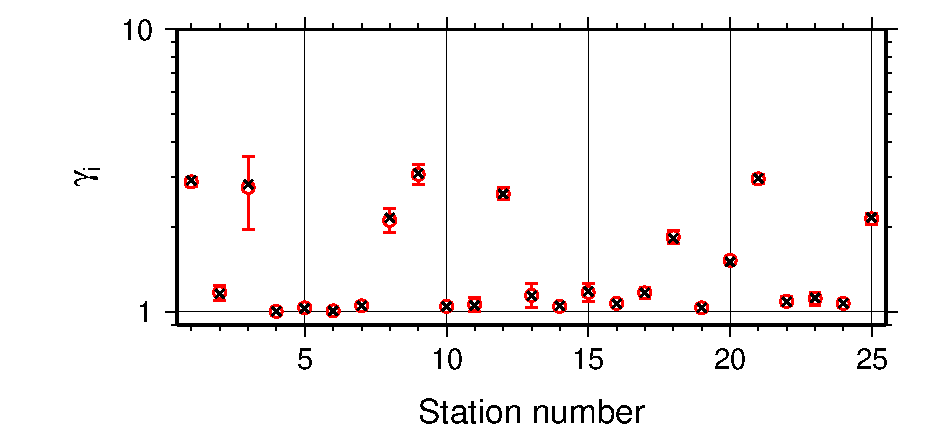
\includegraphics[scale=\plotdindmeanscale]{\figdir/m02a-lyr11a_cb12-h0a2a-d05a-t01a_dr-e43n42_cb1X_loc-regi0_c-s40k-p0p0-pp1_d13a_distorted-sd3a-gtes_gamma_est_esd}
		\label{fig:gamma_3d_site_estimated}
	}
	\subfigure[]{
		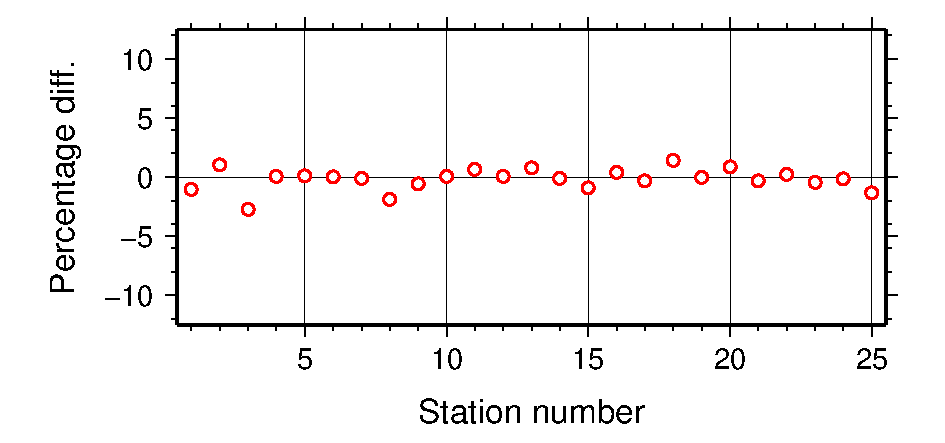
\includegraphics[scale=\plotdindmeanscale]{\figdir/m02a-lyr11a_cb12-h0a2a-d05a-t01a_dr-e43n42_cb1X_loc-regi0_c-s40k-p0p0-pp1_d13a_distorted-sd3a-gtes_gammapdiff_esd.pdf}
		\label{fig:gamma_3d_site_pdiff}
	}
	\caption{Same as Figure \ref{fig:gamma_1d_site} for the 3D example}
	\label{fig:gamma_3d_site}
\end{figure}


%% ==== Regional distortion indicator
%\begin{itemize}
%	\item \red{Regional distortion indicator}
%	\item 
	The regional distortion indicator represents the effect of the shear and splitting parameters throughout the dataset.
	By averaging, the inductive effect from the underlying structure can be flattened out. The regional distortion indicator becomes real-valued, and its magnitude will indicate the strength of shear and splitting parameters on average.
%	\item
	Here, we show the regional distortion indicators from 1D and 3D data distorted with different galvanic distortion strengths (Figure \ref{fig:gamma_regional_example}). They are derived from averaging the local distortion indicators using Eq. \eqref{eq:gamma_regional_def}.
%	\item
	As with the average det and ssq impedances shown in Figure \ref{fig:resp3d_avg_distorted}, the error bar is the SD of local distortion indicators, i.e., it represents the dispersion of the local distortion indicators in each dataset. The stronger galvanic distortion tends to show the larger error bar in this case.
%	\item 
	As with the local distortion indicator, the indicators from 1D data is definitely real-valued, and its magnitude is consistent with the galvanic distortion strength. 
%	\item
	As expected, the regional distortion indicators from distorted 3D datasets are rather real-valued, and its magnitude is comparable to the regional distortion indicators from distorted 1D datasets at the same galvanic distortion strength.
%	\item % Concluding sentence
	In conclusion, the regional distortion indicator can estimate the strength of galvanic distortion -- shear and splitting parameters -- contained in MT datasets fairly well.
%\end{itemize}

%% ==== Gamma regional
\begin{figure}[t]
	\centering
	\subfigure[]{
		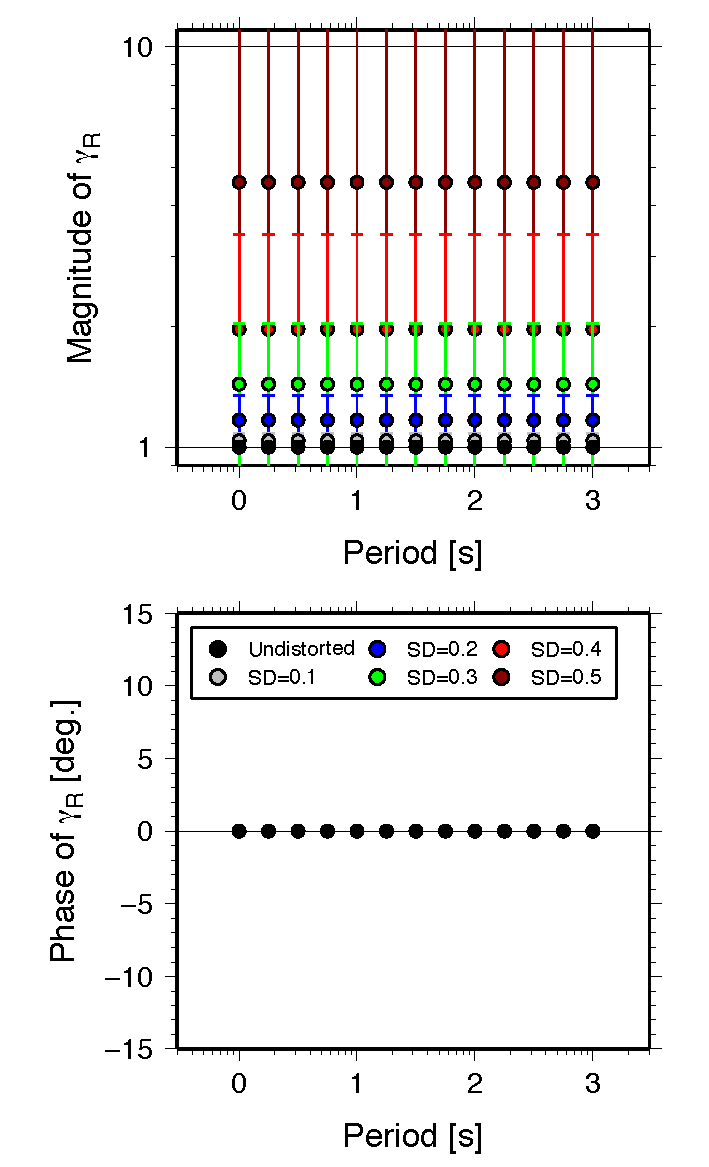
\includegraphics[scale=\plotmtrespscale]{\figdir/lyr11a_n25_d13a_distorted-sdxa_site_dispsd_gamma_magphs.pdf}
		\label{fig:gamma_regional_example_1d}
	}
	\subfigure[]{
		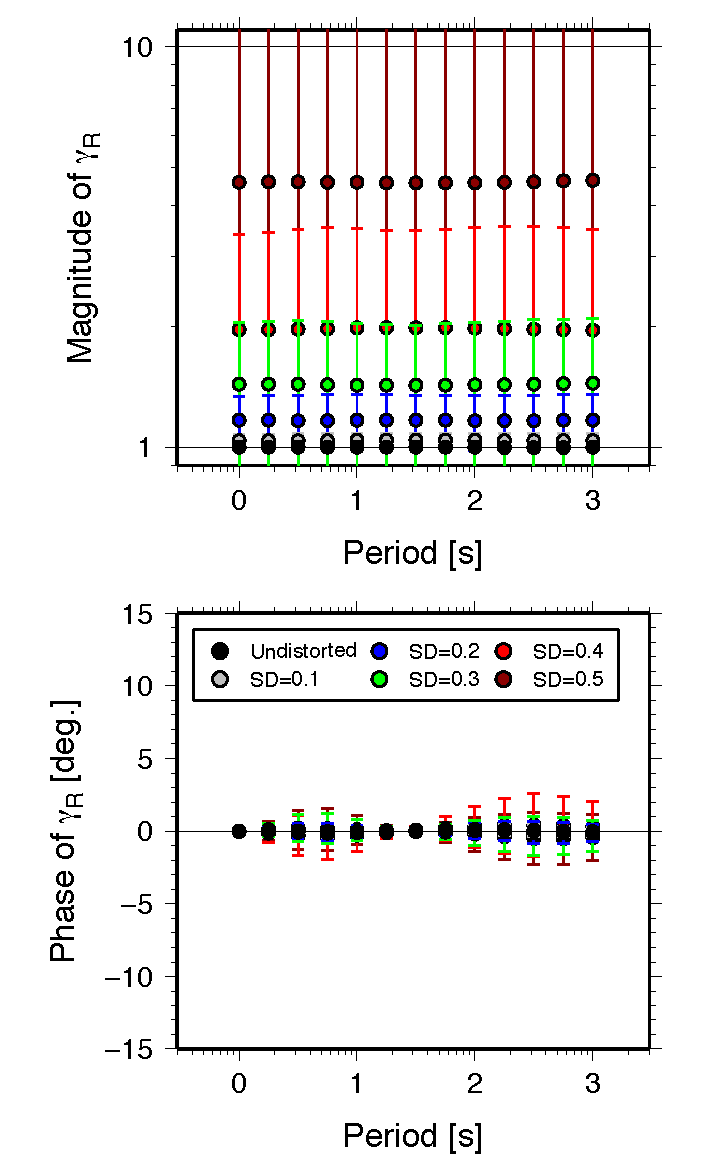
\includegraphics[scale=\plotmtrespscale]{\figdir/m02a-lyr11a_cb12-h0a2a-d05a-t01a_dr-e43n42_cb1X_loc-regi0_c-s40k-p0p0-pp1_d13a_distorted-sdxa_gamma_magphs.pdf}
		\label{fig:gamma_regional_example_3d}
	}
	\caption[Regional distortion indicators from 1D and 3D data distorted with different galvanic distortion strengths]{Regional distortion indicators from (a) 1D and (b) 3D examples with different galvanic distortion strengths.}
	\label{fig:gamma_regional_example}
\end{figure}

%% ==== Concluding paragraph: Local
From the synthetic examples, the local distortion indicator is able to determine the existence and strength of galvanic distortion, if contained in the data.
%
One of its possible and practical uses is to omit or decrease the constraints on the data from the stations that are heavily distorted (e.g., \texttt{syn01} and \texttt{syn02} in the example dataset), if the number of such stations is low.
%
When the number of heavily distorted stations is significant, the regional distortion indicator will be noticeable. The distortion removal or proper treatments, for example, the inversion simultaneously with galvanic distortion \citep[e.g.,][]{sasaki2006a, avdeeva2015a}, may be necessary.
%
However, if the magnitude of regional distortion indicator is rather small, i.e., the whole dataset is weakly distorted, such a complicated computation may be avoided.

%% ==== ====
\begin{comment}
\begin{itemize}
	\item \blue{Additional issues}
	\item \red{As shown in Fig. 25, the regional gamma becomes to be real-valued and frequency independent as a whole, even if local gamma at each site may be complex-valued
and frequency dependent. From this , we can decide whether the dataset is consistent with the assumed setting (regional structure well covered by the observation array + galvanic distorters).
If the regional 3D structure is not well covered, you will have complex-valued and frequency dependent regional gamma.}
\end{itemize}
\end{comment}





\clearpage

% !TEX root = ../../phdthesis_tawatr.tex 
\renewcommand{\thisdir}{_content/appgain}
\renewcommand{\figdir}{\thisdir/_fig}
\section{Apparent gains}

%% ==== Introductory paragraph
%\begin{itemize}
%	\item 
	This section shows the example of apparent det and ssq gains (Eqs. \ref{eq:gdet_def} and \ref{eq:gssq_def}) derived from the synthetic 1D and 3D examples in Sections \ref{sect:example_1d} and \ref{sect:example_3d}, respectively, and we also verify estimating site gain in the data by using the mean apparent gains (Eqs \ref{eq:gdet_mean_def} and \ref{eq:gssq_mean_def}).
%\end{itemize}

%% ==== App gain 008 example
\begin{figure}[!b]
	\centering
	\subfigure[]{
		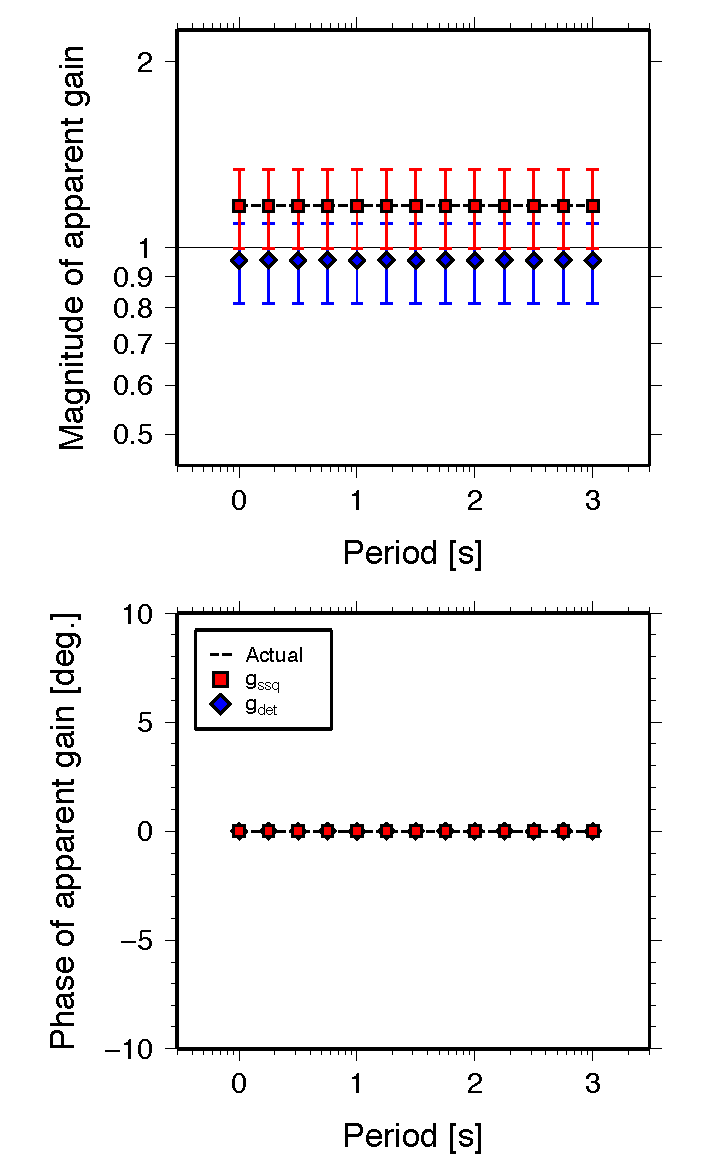
\includegraphics[scale=\plotmtrespscale]{\figdir/lyr11a_d10a_syn0203_gaina_magphs.pdf}
		\label{fig:appgain_example_1d}
	}
	\subfigure[]{
		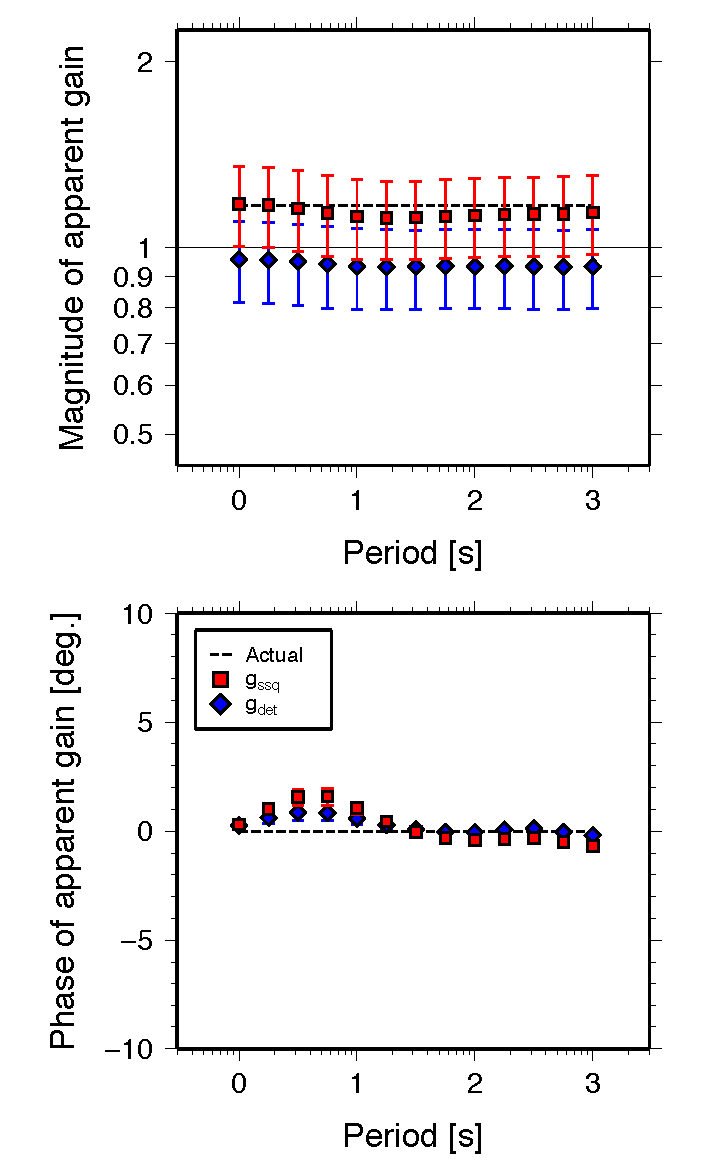
\includegraphics[scale=\plotmtrespscale]{\figdir/m02a-lyr11a_cb12-h0a2a-d05a-t01a_dr-e43n42_cb1X_loc-regi0_c-s40k-p0p0-pp1_d13a_syni0203_gaina_magphs.pdf}
		\label{fig:appgain_example_3d}
	}
	\caption[Example of apparent gains from 1D and 3D data]{Det (diamonds) and ssq (squares) apparent gains from (a) the 1D data and (b) station \texttt{syn08} in the 3D data. The distortion parameters with an SD of 0.3 are applied to both 1D and 3D datasets. 
	A synthetic site gain (dashed line) of 1.20 was applied at this station.}
	\label{fig:appgain_example}
\end{figure}

%% ==== Apparent gains
First, we show the examples of the apparent gains from the 1D data and 3D data at the station \texttt{syn08}. These data are distorted with the distortion parameters $\gtes$ is $(1.20, 0.11, -0.37, 0.49)$ (Figure \ref{fig:appgain_example}). 
%
As proven, the apparent gains from 1D data are real-valued and frequency independent. The apparent ssq gain accurately estimates the synthetic site gain, while the apparent det gain, here, is biased downward because of shear and splitting parameters (Figure \ref{fig:appgain_example_1d}). 
%
In the 3D case, the apparent gains show frequency dependent features and become weakly complex-valued number due to the inductive effect of the underlying 3D heterogeneity (Figure \ref{fig:appgain_example_3d}). 
%
However, the apparent ssq gain still agrees with the synthetic site gain within the uncertainty. As with the 1D example, the apparent det gain is biased downward by the distortion parameters. 
%
Note that the error bars (in Figure \ref{fig:appgain_example}) are derived from the standard error obtained from averaging the det and ssq impedances (Figure \ref{fig:resp3d_avg_distorted}). 
Therefore, if the distortion is very intense, the apparent gains will be less constrained.



%% ==== 
%\begin{itemize}
%\item
The apparent det and ssq gains as a function of period from the 3D datasets distorted with the distortion parameters with an SD of 0.3 are shown in Figure \ref{fig:appgain_3d_distorted}.
The apparent gains have a combination of the frequency dependence and independence.
The frequency-independent feature is upto the site gain contained at each station, while the frequency-dependent feature strongly depends on how strong the inductive effect of the underlying 3D structure is.



%% ==== gssq 3-D individual all 
\begin{figure}[t]
	\centering
	\subfigure[]{
		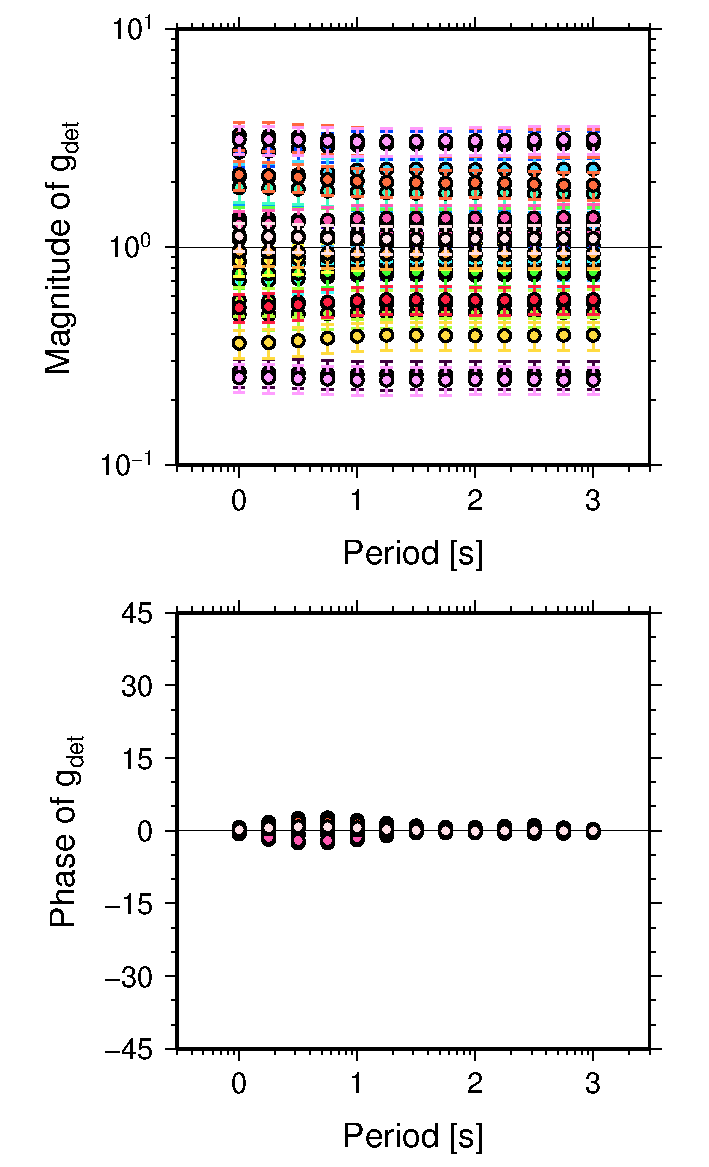
\includegraphics[scale=\plotmtrespscale]{\figdir/m02a-lyr11a_cb12-h0a2a-d05a-t01a_dr-e43n42_cb1X_loc-regi0_c-s40k-p0p0-pp1_d13a_distorted-sd3a-gtes_gdet_magphs.pdf}
		\label{fig:appgain_3d_distorted_gdet}
	}
	\subfigure[]{
		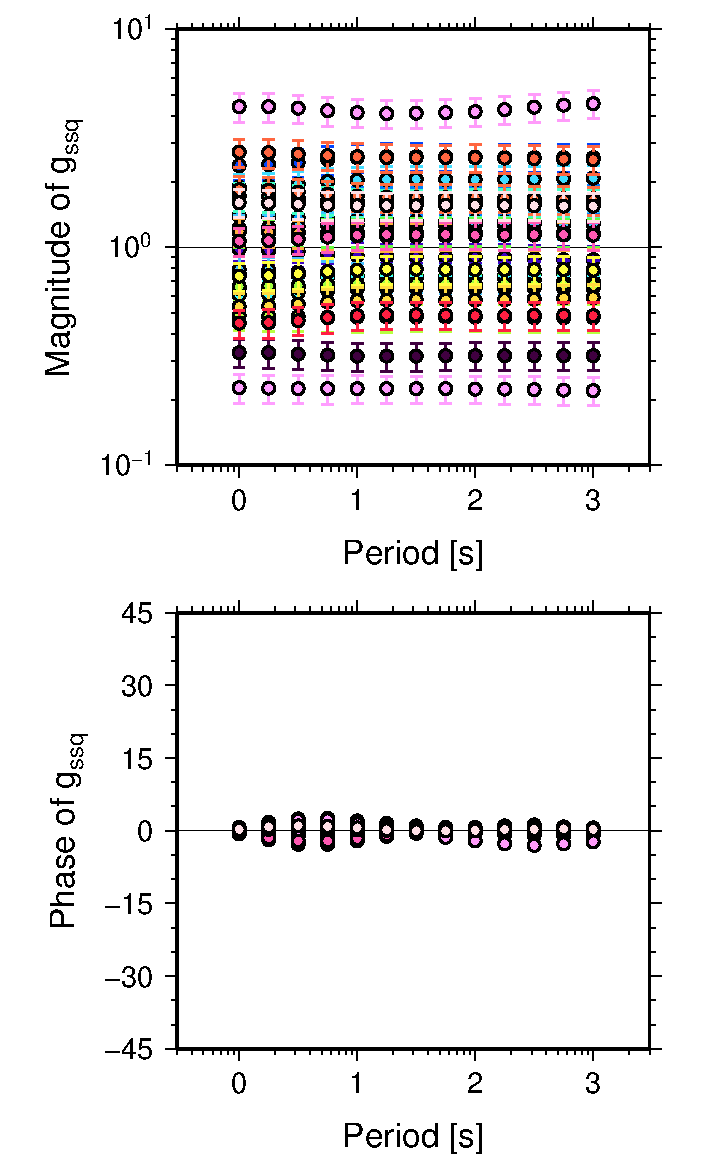
\includegraphics[scale=\plotmtrespscale]{\figdir/m02a-lyr11a_cb12-h0a2a-d05a-t01a_dr-e43n42_cb1X_loc-regi0_c-s40k-p0p0-pp1_d13a_distorted-sd3a-gtes_gssq_magphs.pdf}
		\label{fig:appgain_3d_distorted_gssq}
	}
	\caption[Apparent det and ssq gains from 3D dataset]{The apparent (a) det and (b) ssq gains derived from the 3D example, where a set of distortion parameters with an SD of 0.3 was applied.}
	\label{fig:appgain_3d_distorted}
\end{figure}

%% ==== Mean apparent gains
%\item 
However, to yield the more meaningful interpretation of them,
we calculate the mean apparent ssq and det gains using Eqs \eqref{eq:gdet_mean_def} and \eqref{eq:gssq_mean_def}. 
%\item 
To validate the mean apparent gains, we also define the percentage difference between the mean apparent gains (Eqs \ref{eq:gdet_mean_def} and \ref{eq:gssq_mean_def}) and the synthetic site gain $\gainpi$:
	\begin{equation}
		\mathcal{P}(\gssqimean) = \frac{\gssqimean - \gainpi}{\gainpi} \times 100\%
	\end{equation}	
	\begin{equation}
		\mathcal{P}(\gdetimean) = \frac{\gdetimean - \gainpi}{\gainpi} \times 100\%.
	\end{equation}
%\end{itemize}

%% Mean apparent gain 1D
%\begin{itemize}
%	\item
	From the 1D dataset, the mean apparent ssq gain correctly estimates the synthetic site gain in the data as confirmed by the zero percentage difference (Figure \ref{fig:appgain_1d_site}).
	Conversely, the mean apparent det gain would be either the overestimate or the underestimate of the site gain depending on the galvanic distortion strength, which could be pointed out by the local distortion indicator at individual sites (Figures \ref{fig:gamma_1d_site} and \ref{fig:gamma_3d_site}). This is because the det impedance is affected by the shear and splitting parameters.
	If the distortion at sites is stronger than average, the mean apparent det gain will be an underestimate (e.g., \texttt{syn01}, \texttt{syn03}, \texttt{syn09}). On the contrary, if the distortion at sites is weaker than average, the mean apparent det gain will be an overestimate (e.g., \texttt{syn04}, \texttt{syn05}).
	Note that error bars in this figure are derived from the error propagation rule when calculating Eqs. \eqref{eq:gdet_mean_def} and \eqref{eq:gssq_mean_def}.
	Although the mean apparent det gain agrees with the actual value within the uncertainty range, the mean apparent ssq gain is sitll the favorable choice.
%\end{itemize}

%% Mean 3D
%\redb{Mean 3D}
%\begin{itemize}
%\item
As shown before, the inductive effect from 3D structure can cause the frequency-dependent variation in the apparent gains (Figure \ref{fig:appgain_1d_site}). It may result in some error in estimating the site gain with the mean apparent gain. 
For instance, the mean apparent ssq gains from the stations over the conductive structure (e.g., \texttt{syn07}, \texttt{syn19}) underestimate the synthetic site gains, i.e., less than the actual value (Figure \ref{fig:appgain_3d_site}), as seen from the negative percentage difference.
On the contrary, if the stations are located over the resistive structure (e.g., \texttt{syn04}, \texttt{syn09}), the mean apparent gain is overestimated.
%
Despite of this, the estimate of site gain from the mean apparent ssq gain still agrees with the synthetic values within the statistical uncertainty.
%
%It should be noted that these errors also occur with the apparent det gain, but they are better observed from the apparent ssq gain because the ssq impedance is less sensitive to the galvanic distortion.
%\end{itemize}

%% ==== Concluding paragraph
%\begin{itemize}
%	\item \red{concluding paragraph}
%	\item 
	It is believed that the site gain is undeterminable without other independent geophysical data \citep[e.g.,][]{groom1993a, bibby2005a}.
%	\item 
	From the theoretical derivation and the synthetic examples, the apparent ssq gain is shown to be the promising parameter for the site gain estimation. 
	It is also important to note that this information can be gleaned from MT data alone.
	This parameter would help correcting the magnitude of MT impedances.	
%\end{itemize}

%% ==== App gain 1-D: Percentage difference
\begin{figure}[t]
	\centering
	\subfigure[]{
		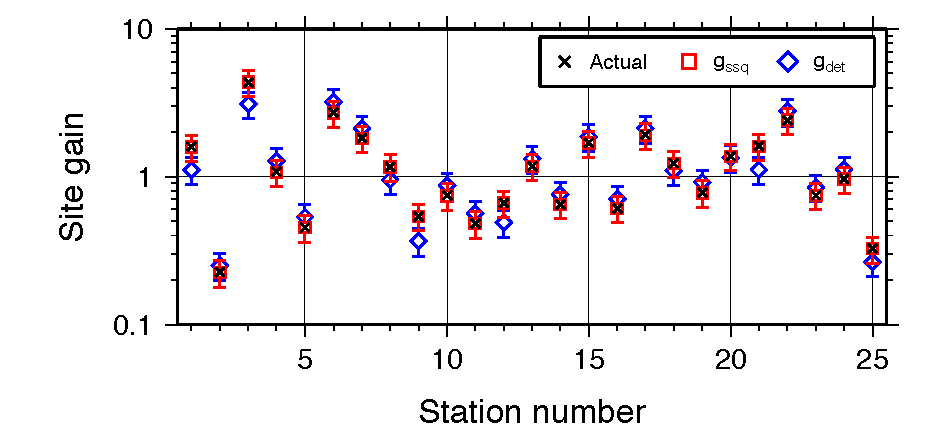
\includegraphics[scale=\plotdindmeanscale]{\figdir/lyr11a_n25_d13a_distorted-sd3a-gtes_gaina_est.pdf}
		\label{fig:appgain_1d_site_estimated}
	}
	\subfigure[]{
		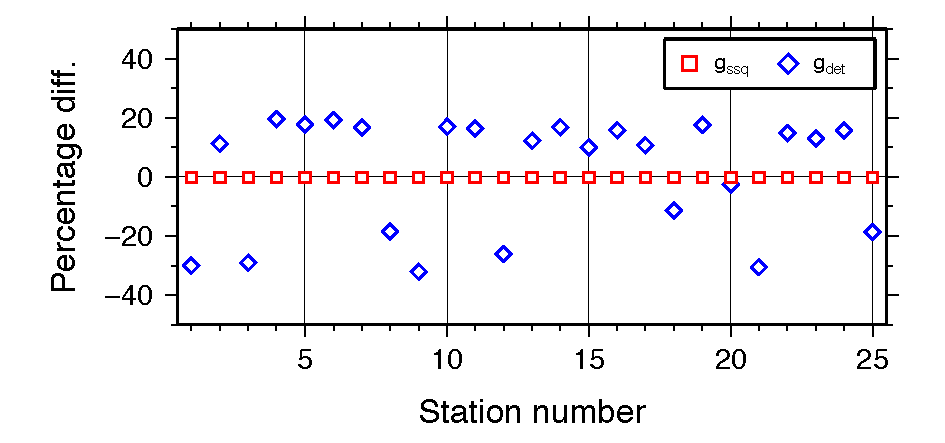
\includegraphics[scale=\plotdindmeanscale]{\figdir/lyr11a_n25_d13a_distorted-sd3a-gtes_gaina_est_diffp.pdf}
		\label{fig:appgain_1d_site_pdiff}
	}
	\caption[Comparison of the actual and the mean apparent gains from 1D dataset]{(a) Comparison of actual site gains (crosses) with the mean apparent det (diamonds) and ssq (squares) gains from the 1D example, where a set of distortion parameters with an SD of 0.3 was applied. (b) Percentage difference between the mean apparent gains and the actual site gains}
	\label{fig:appgain_1d_site}
\end{figure}

%% ==== App gain 3-D: Percentage difference
\begin{figure}[t]
	\centering
	\subfigure[]{
		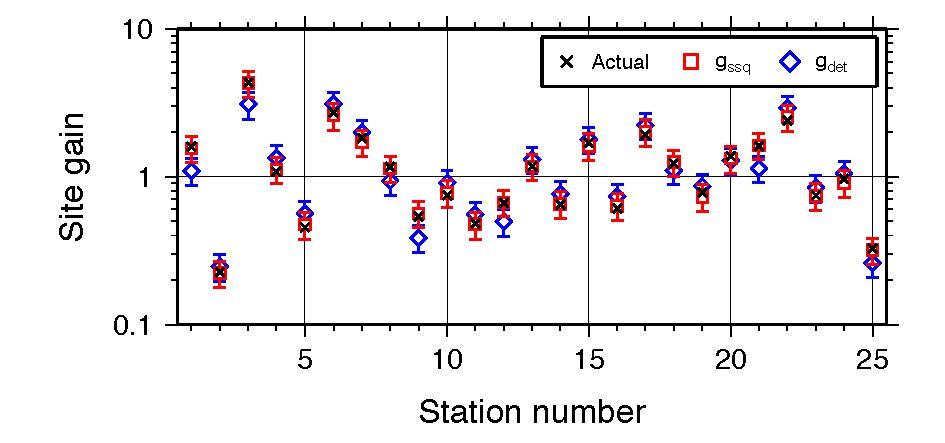
\includegraphics[scale=\plotdindmeanscale]{\figdir/m02a-lyr11a_cb12-h0a2a-d05a-t01a_dr-e43n42_cb1X_loc-regi0_c-s40k-p0p0-pp1_d13a_distorted-sd3a-gtes_gaina_est.pdf}
		\label{fig:appgain_3d_site_estimated}
	}
	\subfigure[]{
		\includegraphics[scale=\plotdindmeanscale]{\figdir/m02a-lyr11a_cb12-h0a2a-d05a-t01a_dr-e43n42_cb1X_loc-regi0_c-s40k-p0p0-pp1_d13a_distorted-sd3a-gtes_gaina_est_diffp.pdf}
		\label{fig:appgain_3d_site_pdiff}
	}
	\caption{Same as Figure \ref{fig:appgain_1d_site} for the 3D example}
	\label{fig:appgain_3d_site}
\end{figure}


%\clearpage
%
% !TEX root = ../../phdthesis_tawatr.tex 
\renewcommand{\thisdir}{_content/htr_test}
\renewcommand{\figdir}{\thisdir/_fig}
\section{Examining the near-surface small-scale heterogeneity model}


\blueb{Introductory paragraph}
\begin{itemize}
	\item In the previous sections, we simulated the galvanic distortion with the random galvanic distortion parameters -- site gain, twist, shear and splitting parameters.
	\item In this section, we used the near-surface small-scale heterogeneity to represent the galvanic distortion effect in order to imitate the situation illustrated in Figure \ref{fig:galvanic_distortion_model}, which we may face in reality.
	\item The model of small-scale heterogeneity (Figure \ref{fig:htr_model}) was added to our 3D model (Figure \ref{fig:model3d_setting}) at the near-surface layer.
	The distribution of the resistivity of the small-scale heterogeniety model is assumed to be the normal distribution with the SD of XX and bounded within $(-XXX,XXX)$ in logarithmic scale (Figure \ref{fig:XXX}). The layer of heterogeneity was extended from the surface to XXX m depth. The MT array configuration remains the same as used in the 3D example (Figure \ref{fig:model3d_setting}).
	\item The models of the regional mean 1D conductivity profile from the average det and ssq impedances were shown in comparison with the 3D example without the near-surface heterogeneity layer. Also, the implication of  local and regional distortion indicators and the apparent gains was presented.
\end{itemize}

\blueb{Show the plots of results. Describe it and discussion.}
\begin{itemize}
	\item Showing the example of det and ssq from one stations probably the same station as in 3D example.
	\item Showing the det and ssq impedances from the whole clusters
	\item Showing the average det and ssq impedances from this model in comparison with the results from the model without the near-surface layer.
	\item Showing the local and regional distortion indicators.
	\item Showing the apparent gains.
\end{itemize}

\begin{figure}
	\centering
	\includegraphics[scale=\plotdindmeanscale]{\figdir/htr_model.pdf}
	\caption{Example of the heterogeneity model. (Just an example) Here the heterogeneity size is 2.5 km x 2.5 km}
	\label{fig:htr_model}	
\end{figure}


\clearpage

% !TEX root = ../../phdthesis_tawatr.tex 
\renewcommand{\thisdir}{_content/conclusions}
\renewcommand{\figdir}{\thisdir/_fig}
\chapter[Conclusions]{Conclusions}

%\begin{itemize}
%	\item 
%	The optimal model of the regional mean 1D conductivity profile would be a good 
%	Any conductivity distribution can be expressed as the regional mean 1D conductivity profile and the lateral conductivity contrast. 
%	\item 
%	\red{
	One strategy in performing 3D inversion is to start by searching for a reliable model of the regional mean 1D conductivity profile which is able to minimize the variance of the conductivity contrast. 
%	}
%	\item 
	Traditionally, the model of the regional mean 1D conductivity profile was estimated from the Berdichevsky average, i.e., the average det impedance, which is able to smooth out the galvanic effect from small-scale local structure. However, it had been introduced before the knowledge of galvanic distortion was well established. Therefore, the effect of the galvanic distortion on the Berdichevsky average has never been examined.
%\end{itemize}

%\begin{itemize}
%	\item 
	Galvanic distortion is the spatial aliasing in MT data by small-scale near-surface heterogeneity, and it is unavoidable in general.
%	\item 
	The question is how reliable is the model obtained from the Berdichevsky average with the presence of galvanic distortion.
%	\item 
	The ssq impedance is therefore introduced as another rotation invariant candidate to challenge this problem.
%	\item 
	The det and ssq impedances derived from the distorted MT impedance are algebraically examined using the Groom--Bailey model of galvanic distortion.
%	\item 
	It is found that the det impedance is biased downward by the shear and splitting parameters, while the ssq impedance is less sensitive to these distortion parameters.
%	\item 
	This major finding urges us to redefine the Berdichevsky average with the ssq impedance in order to reliably estimate the model of the regional mean 1D conductivity profile.
%	\item 
	From the synthetic examples, the models obtained from the traditional Berdichevsky average may overestimate the regional mean 1D conductivity profile.
 Regardless of the galvanic distortion strength, the average ssq impedance is theoretically and numerically proven to be the promising method to accurately estimate the model of the regional mean 1D conductivity profile.

%% ==== Theoretical def
%\begin{itemize}
%	\item 
	The definitions for the theoretical model of the regional mean 1D conductivity profile are also introduced. 
%	\item 
	Instead of comparing the estimated model with the host background, which is not viable in reality, we are able to compare the estimated model with the theoretical model from the given definitions.
%	\item 
	The theoretical model could be calculated using either a linear or logarithmic scale average depending on the choice of model parameters in optimization.
%	\item 
	The numerical results show that the theoretical models are consistent with the estimated model when the MT array is larger than the anomaly size. 
%	\item 
	Therefore, the theoretical and estimated model of the regional mean 1D conductivity profile is reliable with the appropriate size of MT array.
%\end{itemize}

%% ==== Distortion indicators: Local and Regional
%\begin{itemize}
%	\item 
	In addition, the concept of galvanic distortion-related parameters was first introduced.
%	\item 
	Using these parameters enables us	to indicate the existence of galvanic distortion and also to quantify its strength. 
%	\item 
	Two type of indicators are defined from the det and ssq impedances, the local and regional distortion indicators and the apparent gains. Their functions are totally different. The former is to indicate the strength of the shear and splitting effect, and the latter is to be a good approximate of site gain, which is generally claimed to be the undeterminable distortion parameter.
%	\item 
	Note that the effect of twist cannot be ascertained because both det and ssq impedance are rotationally invariant.
%	\item 
	One possible and practical use of the local distortion indicator is to point out heavily distorted MT data, which may be rejected in interpretation. The regional distortion indicator can be used to determine the necessity of the proper treatment or removal of galvanic distortion, which may be algebraically complicated and computationally expensive. 	
%\end{itemize}


%% ==== Concluding paragraph
%\begin{itemize}
%	\item 
%\red{
	The ultimate goal of this thesis is to handle the problem of galvanic distortion, particularly in imaging 3D conductivity structure.
	In conclusion, we propose to estimate the model of the regional mean 1D conductivity profile, less biased by the galvanic distortion, with the average ssq impedance and make the distortion strength quantifiable with the galvanic distortion indicators. 
	The theoretical derivation of them was verified by a series of synthetic examples.
	With the proposed method, the unbiased models of the regional mean 1D conductivity profile could be obtained even if the datasets are distorted.
	The galvanic distortion indicators would help determine the need of applying the augmented approach, e.g., 3D inversion including galvanic distortion, or the omission of heavily distorted data.
%	\item
%	\item 
	The proposed method to reliably estimate the model of the regional mean 1D conductivity profile from the set of distorted MT data and the concept of galvanic distortion indicators would be essential and instructive in 3D inversion.
%	}
		
%\end{itemize}



%\clearpage
%
% !TEX root = ../thesis_phd.tex 

\chapter{Unused topics and materials}
	\red{Check whether the definition of static shift is given}.
	
	\section{Intro}
\begin{itemize}
	\item \redb{(The theoretical model of regional mean 1-D profile was examined in Section XXX) [Have no idea where to place it]}
	\item The choices of choosing the initial and also \emph{a priori} models yet remain controversial. 
	\item \red{Writing the conductivity distribution in this way, the anomaly is represented by the conductivity contrast.}
	\item The regional structure is changed with changing frequency range.
	\item However, the definition of the regional conductivity profile, $\sigma_\Regional$, is never explicitly given. In this work we present the definition to calculate the theoretical model of regional mean 1-D conductivity profile.
		The small-scale structure confined in near-surface thin, thinner than the inductive scale length, layers is considered as distorter \citep{utada2000a}.
	\item In this work, the regional scale means the structure which its horizontal dimension is comparable to or larger than the inductive scale length of present interest \citep[also see][]{bahr1988a}. 
	\item \citet{tournerie2002a} also use average impedance to estimate the good starting model for 2D inversions	
\end{itemize}
	\section{Galvanic distortion}
	\begin{itemize}
		\item In this context, Small and spatial dependent  $\rightarrow$ assumed random 
		\item Although, the formulation of Groom-Bailey's model was criticized controversial and not intuitively obvious \citep{bibby2005a}, it is \emph{mathematically} possible.
	\end{itemize}	
	\section{Synthetic tests}
	%% ==== Table: Layered-earth model
\begin{table}
	\centering
	\begin{tabular}{ccc}
	\hline 
	Layer & Depth (km) & Resistivity (\Ohmm) \\ \hline
	Surface & 0.0 -- 3.5 & 100 \\
	Upper crust & 3.5 -- 14.8 & 1000 \\
	Lower crust & 14.8 -- 33.3 & 30 \\
	Upper mantle & 33.3 -- 136.0 & 100 \\
	Asthenosphere & 136.0 -- 203.0 & 10 \\
	Upper mantle & 203.0 -- 451.0 & 30 \\
	Mantle transition zone & 451.0 -- 673.0 & 3 \\
	Lower mantle & 673.0 -- $\infty$ & 1 \\ \hline
	\end{tabular}
	\caption{The detail of the layered earth in Figure \ref{fig:example1d_model}.}
	\label{tab:example1d_model}
\end{table}
\subsection{Synthetic 1D}
%% ====
 \red{-- PENDING --}
\begin{itemize}
	\item \red{Add the results showing that if we use the individual (distorted) observation to represent the regional structure, the conductivity contrast may not be minimized.}
\end{itemize}
\subsection{Synthetic 3D}
\begin{itemize}
	\item Add the results showing that if we use the response from different underlying structure may have different
	\item The distorted det impedances in the synthetic tests (Figures \ref{fig:resp1d_individual_all_distorted_sd3a_det} and \ref{fig:resp3d_individual_all_distorted_sd3a_det}) also resemble the results in  \citet{berdichevsky1980a}.	
	
\end{itemize}

\begin{itemize}
	\item The average approach helps flatten the contribution from underlying 3-D structure
\end{itemize}



\bibliographystyle{apa} % if you are using bibtex
    \setlength{\bibsep}{2pt}	% To make the seperation between bibitem
%\bibliography{/Users/tawatr/Research/_bib/_Bib_Induction/_Bib_Induction}
\input{phdthesis_tawatr_picked.bbl}


\biography
\end{document}
